%%
%% This is file `sample-acmsmall-conf.tex',
%% generated with the docstrip utility.
%%
%% The original source files were:
%%
%% samples.dtx  (with options: `acmsmall-conf')
%% 
%% IMPORTANT NOTICE:
%% 
%% For the copyright see the source file.
%% 
%% Any modified versions of this file must be renamed
%% with new filenames distinct from sample-acmsmall-conf.tex.
%% 
%% For distribution of the original source see the terms
%% for copying and modification in the file samples.dtx.
%% 
%% This generated file may be distributed as long as the
%% original source files, as listed above, are part of the
%% same distribution. (The sources need not necessarily be
%% in the same archive or directory.)
%%
%%
%% Commands for TeXCount
%TC:macro \cite [option:text,text]
%TC:macro \citep [option:text,text]
%TC:macro \citet [option:text,text]
%TC:envir table 0 1
%TC:envir table* 0 1
%TC:envir tabular [ignore] word
%TC:envir displaymath 0 word
%TC:envir math 0 word
%TC:envir comment 0 0
%%
%%
%% The first command in your LaTeX source must be the \documentclass
%% command.
%%
%% For submission and review of your manuscript please change the
%% command to \documentclass[manuscript, screen, review]{acmart}.
%%
%% When submitting camera ready or to TAPS, please change the command
%% to \documentclass[sigconf]{acmart} or whichever template is required
%% for your publication.
%%
%%
%\documentclass[sigconf,anonymous]{acmart}
% https://conf.researchr.org/track/esem-2024/esem-2024-technical-track
% All submissions must be written in English and must be submitted via EasyChair
% in the PDF format, and they must be formatted according to the ACM proceedings
% template, which can be found at ACM Proceedings Template (https://www.acm.org/publications/proceedings-template) or in Overleaf at https://www.overleaf.com/gallery/tagged/acm).
\documentclass[sigconf,review,anonymous]{acmart}
\acmConference[ESEC/FSE 2023]{The 31st ACM Joint European Software Engineering Conference and Symposium on the Foundations of Software Engineering}{11 - 17 November, 2023}{San Francisco, USA}
\hypersetup{
   colorlinks=true,
  pdfborder={0 0 0},
}
%%
%% \BibTeX command to typeset BibTeX logo in the docs
\AtBeginDocument{%
  \providecommand\BibTeX{{%
    Bib\TeX}}}


%XXXXXXXXXXXXXX
\newcommand{\mytitle}{Empirical Evaluation of Frequency Based Statistical Models for Estimating Killable Mutants}

% ALESSIO: A Large Empirical Evaluation of Frequency Based Statistical Models for Estimating Killable Mutants
% ALESSIO: Empirically Evaluating Frequency Based Statistical Models for Estimating Killable Mutants
% ALESSIO: A Large Empirical Evaluation of Frequency Based Statistical Models applied to Mutation Testing

% ALESSIO: Check whether we use "Frequency Based Statistical Models" in the paper or something else (e.g., "Bio-Inspired Estimators")


%Estimating Equivalent Mutants: Are we there yet?}
%\newcommand{\mytitle}{Estimating Equivalent Mutants: Are we there yet?}
%\usepackage{hyperref}
%\usepackage{xcolor}
\definecolor{rltred}{rgb}{0.5,0,0}
\definecolor{rltgreen}{rgb}{0,0.5,0}
\definecolor{rltblue}{rgb}{0,0,0.5}
\hypersetup{
colorlinks=true,
urlcolor=rltblue, % was rltblue
linkcolor=rltblue,
citecolor=rltblue,
filecolor=rltblue,         % color of file links
pdftitle={\mytitle}
}
\newif\ifdraft\drafttrue
\newif\iflong\longfalse

\definecolor{eclipseBlue}{RGB}{42,0.0,255}
\definecolor{eclipseGreen}{RGB}{63,127,95}
\definecolor{eclipsePurple}{RGB}{127,0,85}
\definecolor{darkgreen}{RGB}{1,50,32}

\usepackage[procnames]{listings}
\lstdefinestyle{python}
{
    breaklines=false,
    basicstyle=\footnotesize\ttfamily,
    numberblanklines=false,
    language=python,
    tabsize=2,
    commentstyle=\color{eclipseGreen},
    keywordstyle=\bfseries\color{eclipsePurple},
    stringstyle=\color{eclipseBlue},
    procnamestyle=\bfseries\color{black},
    procnamekeys={def},
    columns=flexible,
    identifierstyle=
}
\usepackage{tcolorbox}
\usepackage{amsfonts}

\definecolor{codegreen}{rgb}{0,0.6,0}
\definecolor{codegray}{rgb}{0.5,0.5,0.5}
\definecolor{codepurple}{rgb}{0.58,0,0.82}
\definecolor{codeorange}{rgb}{1,0.5,0}
\definecolor{backcolour}{rgb}{0.95,0.95,0.92}

\lstdefinestyle{mystyle}{
    % backgroundcolor=\color{backcolour},
    commentstyle=\color{codegreen},
    keywordstyle=\color{magenta},
    numberstyle=\tiny\color{codegray},
    stringstyle=\color{codepurple},
    basicstyle=\linespread{0.8}\ttfamily,
    breakatwhitespace=false,
    breaklines=true,
    captionpos=b,
    keepspaces=true,
    numbers=left,
    numbersep=5pt,
    showspaces=false,
    showstringspaces=false,
    showtabs=false,
    tabsize=2
}

\lstset{style=mystyle}
% The name of our central contribution, with variations
\usepackage{xspace}

%%%%
%
%
% How Many estimators do we consider?
%
%
%%%%
\newcommand{\estimatorCount}{twelve\xspace}
\newcommand{\projectCount}{ten\xspace}
\newcommand{\mutantCount}{110595\xspace}

\newcommand{\rA}{\textsc{R$_\text{A}$}\xspace}
\newcommand{\rB}{\textsc{R$_\text{B}$}\xspace}
\newcommand{\rC}{\textsc{R$_\text{C}$}\xspace}

\newcommand{\ICEallrare}{ICE-k0\xspace}
\newcommand{\Zelterman}{Zelterman\xspace}
\newcommand{\ChaoBunge}{Chao Bunge\xspace}
\newcommand{\Jackknife}{Jackknife\xspace}
\newcommand{\Chao}{Chao\xspace}
%\newcommand{\Chaobiascorrected}{Chao-bc\xspace}
\newcommand{\improvedChao}{iChao\xspace}
\newcommand{\ICE}{ICE\xspace}
\newcommand{\improvedICE}{ICE-1\xspace}
\newcommand{\Unpmle}{UNPMLE\xspace}
\newcommand{\Bootstrap}{Bootstrap\xspace}
\newcommand{\Pnpmle}{PNPMLE\xspace}
\newcommand{\PCG}{PCG\xspace}


\newcommand{\chao}{$\hat{S}_\textit{Chao}$\xspace}

\newcounter{todocounter}
\newcommand{\todo}[1]{\marginpar{$|$}\textcolor{red}{\stepcounter{todocounter}\footnote[\thetodocounter]{\textcolor{red}{\textbf{TODO }}\textit{#1}}}}
\newcommand{\repl}[2]{\textcolor{red}{\textbf{REPLACE }\st{#1} \textit{#2}}}     
\newcommand{\rem}[1]{\textcolor{red}{\textbf{REMOVED }\st{#1}}}                  
                                                                                 
\newcommand{\done}[1]{\textcolor{green}{\stepcounter{todocounter}\endnote[\thetodocounter]{\textbf{DONE }\textit{#1}}}}

%\renewcommand{\todo}[1]{}
%\renewcommand{\done}[1]{}
%\renewcommand{\rem}[1]{}

\newcommand{\Randoop}{\textsc{Randoop}\xspace}
\newcommand{\Evosuite}{\textsc{EvoSuite}\xspace}
\newcommand{\original}{\textsc{Original}\xspace}
\newcommand{\PIT}{\textsc{PIT}\xspace}

\newcommand{\EvosuiteRandom}{\textsc{Random}\xspace}
%\newcommand{\EvosuiteStd}{\textsc{Evosuite-Standard}\xspace}
\newcommand{\EvosuiteDynamosa}{\textsc{DynaMOSA}\xspace}


\usepackage{cleveref}

%XXXXXXXXXXXXXX
\usepackage{adjustbox}
%\usepackage{graphicx}
\usepackage{pgf,tikz}
\usepackage{endnotes}
\usepackage{pifont}
\usepackage{widetable}
\usepackage{mathtools}
\DeclarePairedDelimiter{\ceil}{\lceil}{\rceil}
\usepackage{doi}
%\usepackage{microtype}
\usepackage{forest}
%\usepackage{comment}
\usepackage{footmisc}
\usepackage[noend]{algpseudocode}
\usepackage{algorithm}
\usepackage{algorithmicx}
\usepackage{epstopdf}
\usepackage{textcomp}
\usepackage{boxedminipage}
\usepackage{float}
\usepackage{soul}
\usepackage{alltt}
%\usepackage{caption}

%\usepackage{mdwtab}
\usepackage{syntax}
\usepackage{lstautogobble}
\usepackage{qtree}

\Crefname{figure}{Fig.}{Figs.}
\Crefname{equation}{Eqn.}{Eqns.}
\crefname{section}{Section}{Sections}
\crefname{subsection}{Section}{Sections}
\Crefname{Algorithm}{Alg.}{Algs.}

\usepackage{subcaption}
\usepackage{multirow}

%\usepackage{balance}
\usepackage[inline]{enumitem}
\usetikzlibrary{shapes.misc, positioning}

\usepackage{url}
%\usepackage{booktabs}

\usepackage{amsmath}
%\usepackage{amssymb}

\newcommand{\B}[1]{\textbf{#1}}

\newcommand{\Coreutils}{UNIX command line utilities\xspace}

\algblockdefx[switch]{Switch}{EndSwitch}%
[1]{\textbf{switch} #1}%
{}%
\algloopdefx{Case}[1]{\textbf{case} #1:}%
\algdef{SE}[DOWHILE]{Do}{doWhile}{\algorithmicdo}[1]{\algorithmicwhile\ #1}%

\algnewcommand\RETURN{\State \algorithmicreturn}%

\usepackage{contour}
\usepackage[normalem]{ulem}

\renewcommand{\ULdepth}{1.8pt}
\contourlength{0.8pt}

\newcommand{\myuline}[1]{%
  \uline{\phantom{#1}}%
  \llap{\contour{white}{#1}}%
}

\newenvironment{result}%
{\medskip
\noindent
\let\emph=\textbf\begin{center}
\begin{boxedminipage}{\columnwidth}\begin{center}\em}%
{\end{center}\end{boxedminipage}\end{center}%
\medskip
}



\def\term#1{\texttt{'\textbf{#1}'}}
\newcommand{\termC}[2]{\texttt{'\textbf{\color{#2}#1}'}}
\def\nonterm#1{\textnormal{\emph{#1}}}
\def\regex#1{\texttt{{\color{blue}/}#1{\color{blue}/}}}
\def\expandsto{\(\rightarrow{}\)}


\definecolor{nontermcolor}{rgb}{0.4, 0.05, 0.0} % dark orange
\definecolor{absnontermcolor}{rgb}{0.4, 0.5, 0.0} % light green
\definecolor{evokcolor}{rgb}{0.8, 0.05, 0.1}    % orange
\definecolor{incorrectcolor}{rgb}{0.5, 0.0, 0.13}
\definecolor{incompletecolor}{rgb}{0.0, 0.0, 0.55}
\definecolor{validcolor}{rgb}{0.33, 0.42, 0.18} %  {0.0, 0.28, 0.67}
\definecolor{retcolor}{rgb}{0.65, 0.16, 0.16}
\definecolor{ipatterncolor}{rgb}{0.0, 0.5, 0.4} % cyan?
\definecolor{termcolor}{rgb}{0.0, 0.05, 0.4}    % dark blue
\definecolor{regexcolor}{rgb}{0.1, 0.3, 0.1}    % dark green

\def\term#1{\texttt{\color{termcolor}'\textbf{#1}'}}
\def\nonterm#1{{\color{nontermcolor}$\langle$\textnormal{\emph{#1}}$\rangle$}}
\def\absnonterm#1{{\color{absnontermcolor}$\langle$\textnormal{\emph{#1}}$\rangle$}}
\def\evoknt#1{{\color{evokcolor}$\langle$\textnormal{\emph{#1}}$\rangle$}}
\def\ipattern#1{\color{ipatterncolor}#1}
\def\regex#1{\texttt{\color{regexcolor}/#1/}}
\def\expandsto{::=}

\newcommand{\cmark}{\ding{51}}%
\newcommand{\xmark}{\ding{55}}%
\newcommand{\dmark}{\ding{108}}%
\def\ret#1{\texttt{\color{retcolor}\textbf{\small#1}}}



\def\Rincomplete{\texttt{\color{incompletecolor}\textbf{$\vartriangleright$}}\xspace}
\def\Rincorrect{\texttt{\color{incorrectcolor}\textbf{$\ntriangleright$}}\xspace}
\def\Rvalid{\texttt{\color{validcolor}\textbf{$\blacksquare$}}\xspace}

\renewcommand{\ulitleft}{\normalfont\ttfamily}
\renewcommand{\litleft}{\bgroup\color{termcolor}`\ulitleft}
\renewcommand{\litright}{\ulitright'\egroup}

\renewcommand{\syntleft}{\bgroup\color{nontermcolor}$\langle$\normalfont\itshape}
\renewcommand{\syntright}{$\rangle$\egroup}

\grammarparsep 3pt plus 1pt minus 1pt

\newenvironment{densegrammar}{%
\begin{small}
\begin{grammar}%
}%
{%
\end{grammar}%
\end{small}%
}
\newenvironment{Grammar}%
{\begin{itemize}\item[]\begin{densegrammar}}%
{\end{densegrammar}\end{itemize}}%


\def\instrumentationless{instrumentationless\xspace}
\def\Pyparsing{\emph{Pyparsing}\xspace}
\def\Gparsing{\emph{General Parsers}\xspace}
\def\|#1|{\textit{#1}}
\def\<#1>{\texttt{#1}}
%\def\[[#1\]]{\texttt{#1}} % better?

% \newcounter{todocounter}
% \newcommand{\todo}[1]{\marginpar{$|$}\textcolor{red}{\stepcounter{todocounter}\footnote[\thetodocounter]{\textcolor{red}{\textbf{TODO }}\textit{#1}}}}
% \newcommand{\repl}[2]{\textcolor{red}{\textbf{REPLACE }\st{#1} \textit{#2}}}
% \newcommand{\rem}[1]{\textcolor{red}{\textbf{REMOVED }\st{#1}}}
% 
% \newcommand{\done}[1]{\textcolor{green}{\stepcounter{todocounter}\endnote[\thetodocounter]{\textbf{DONE }\textit{#1}}}}

\IfFileExists{SUBMIT}{
\renewcommand{\todo}[1]{}
\renewcommand{\done}[1]{}
\renewcommand{\rem}[1]{}
\renewcommand{\theendnotes}{}
}

\definecolor{eclipseBlue}{RGB}{42,0.0,255}
\definecolor{eclipseGreen}{RGB}{63,127,95}
\definecolor{eclipsePurple}{RGB}{127,0,85}

\newcommand{\decoder}{\textsc{Decoder}\xspace}
\newcommand{\decoderNS}{\textsc{Decoder}\xspace}
\newcommand{\pFuzzer}{pFuzzer\xspace}
\newcommand{\pFuzzerNS}{pFuzzer\xspace}
\newcommand{\lFuzzer}{lFuzzer\xspace}
\newcommand{\lFuzzerNS}{lFuzzer\xspace}

\definecolor{eclipseBlue}{RGB}{42,0.0,255}
\definecolor{eclipseGreen}{RGB}{63,127,95}
\definecolor{eclipsePurple}{RGB}{127,0,85}


%\usepackage[procnames]{listings}
\lstdefinestyle{asm}
{
    basicstyle=\footnotesize\ttfamily,
    numberblanklines=false,
    language=assembly,
    tabsize=2,
    commentstyle=\color{eclipseGreen},
    keywordstyle=\bfseries\color{eclipsePurple},
    stringstyle=\color{eclipseBlue},
    procnamestyle=\bfseries\color{black},
    numbers=none,
    procnamekeys={},
    columns=flexible,
    xleftmargin=3mm,
    framexleftmargin=1mm,
    identifierstyle=
}
\lstdefinestyle{python}
{
    basicstyle=\footnotesize\ttfamily,
    numberblanklines=false,
    language=python,
    tabsize=2,
    commentstyle=\color{eclipseGreen},
    keywordstyle=\bfseries\color{eclipsePurple},
    stringstyle=\color{eclipseBlue},
    procnamestyle=\bfseries\color{black},
    morekeywords={where,match,case},            % if you want to add more keywords to the set
    numbers=left,
    procnamekeys={def},
    columns=flexible,
    xleftmargin=3mm,
    framexleftmargin=1mm,
    identifierstyle=
}

\definecolor{codegreen}{rgb}{0,0.6,0}
\definecolor{codegray}{rgb}{0.5,0.5,0.5}
\definecolor{codepurple}{rgb}{0.58,0,0.82}
\definecolor{backcolour}{rgb}{0.95,0.95,0.92}

\lstdefinestyle{mystyle}{
    % backgroundcolor=\color{backcolour},
    basicstyle=\footnotesize\ttfamily,
    commentstyle=\color{codegreen},
    keywordstyle=\color{eclipsePurple},
    escapeinside={(*}{*)},          % if you want to add LaTeX within your code
    %numberstyle=\tiny\color{codegray},
    stringstyle=\color{codepurple},
    %basicstyle=\linespread{0.8}\ttfamily,
    breakatwhitespace=false,
    breaklines=true,
    captionpos=b,
    keepspaces=true,
    %numbers=left,
    %numbersep=5pt,
    %procnamestyle=\bfseries\color{black},
    %procnamekeys={where},
    morekeywords={where},            % if you want to add more keywords to the set
    showspaces=false,
    showstringspaces=false,
    showtabs=false,
    tabsize=2,
    deletekeywords={expected},
    morestring=[b]' % defines that strings are enclosed in quotes
}

\lstset{style=mystyle}


\newcommand{\pdtg}{parser-directed fuzzing\xspace}
\newcommand{\Pdtg}{Parser-directed fuzzing\xspace}
\newcommand{\pdtgN}{\textsc{pFuzzer}\xspace}
\newcommand{\KLEE}{KLEE\xspace}
\newcommand{\AFL}{AFL\xspace}
\newcommand{\AFLp}{AFL++\xspace}
\newcommand{\AFLplain}{AFL (\<-n>)\xspace}
\newcommand{\AFLW}{AFL with Waypoints\xspace}

\algblockdefx[switch]{Switch}{EndSwitch}%
[1]{\textbf{switch} #1}%
{}%
\algloopdefx{Case}[1]{\textbf{case} #1:}%
\algdef{SE}[DOWHILE]{Do}{doWhile}{\algorithmicdo}[1]{\algorithmicwhile\ #1}%


\newcommand{\json}{\textsc{json}\xspace}
\newcommand{\csv}{\textsc{csv}\xspace}
\newcommand{\ini}{\textsc{ini}\xspace}
\newcommand{\tinyc}{\textsc{tinyC}\xspace}
\newcommand{\mjs}{\textsc{mjs}\xspace}
\newcommand{\SC}{Statement Coverage\xspace}
\newcommand{\BC}{Branch Coverage\xspace}
\def\BibTeX{{\rm B\kern-.05em{\sc i\kern-.025em b}\kern-.08em
    T\kern-.1667em\lower.7ex\hbox{E}\kern-.125emX}}

%% Rights management information.  This information is sent to you
%% when you complete the rights form.  These commands have SAMPLE
%% values in them; it is your responsibility as an author to replace
%% the commands and values with those provided to you when you
%% complete the rights form.
\setcopyright{acmcopyright}
\copyrightyear{2018}
\acmYear{2018}
\acmDOI{XXXXXXX.XXXXXXX}

%% These commands are for a PROCEEDINGS abstract or paper.
\acmConference[Conference acronym 'XX]{Make sure to enter the correct
  conference title from your rights confirmation emai}{June 03--05,
  2018}{Woodstock, NY}
%%
%%  Uncomment \acmBooktitle if the title of the proceedings is different
%%  from ``Proceedings of ...''!
%%
%%\acmBooktitle{Woodstock '18: ACM Symposium on Neural Gaze Detection,
%%  June 03--05, 2018, Woodstock, NY}
\acmPrice{15.00}
\acmISBN{978-1-4503-XXXX-X/18/06}


%%
%% Submission ID.
%% Use this when submitting an article to a sponsored event. You'll
%% receive a unique submission ID from the organizers
%% of the event, and this ID should be used as the parameter to this command.
%%\acmSubmissionID{123-A56-BU3}

%%
%% For managing citations, it is recommended to use bibliography
%% files in BibTeX format.
%%
%% You can then either use BibTeX with the ACM-Reference-Format style,
%% or BibLaTeX with the acmnumeric or acmauthoryear sytles, that include
%% support for advanced citation of software artefact from the
%% biblatex-software package, also separately available on CTAN.
%%
%% Look at the sample-*-biblatex.tex files for templates showcasing
%% the biblatex styles.
%%
%\usepackage[style=ACM-Reference-Format,backend=bibtex,sorting=none]{biblatex}
%%
%% The majority of ACM publications use numbered citations and
%% references.  The command \citestyle{authoryear} switches to the
%% "author year" style.
%%
%% If you are preparing content for an event
%% sponsored by ACM SIGGRAPH, you must use the "author year" style of
%% citations and references.
%% Uncommenting
%% the next command will enable that style.
%%\citestyle{acmauthoryear}


%%
%% end of the preamble, start of the body of the document source.
\begin{document}

%%
%% The "title" command has an optional parameter,
%% allowing the author to define a "short title" to be used in page headers.
\title{\mytitle}

%%
%% The "author" command and its associated commands are used to define
%% the authors and their affiliations.
%% Of note is the shared affiliation of the first two authors, and the
%% "authornote" and "authornotemark" commands
%% used to denote shared contribution to the research.

%\author{Ben Trovato}
%\authornote{Both authors contributed equally to this research.}
%\email{trovato@corporation.com}
%\orcid{1234-5678-9012}
%\author{G.K.M. Tobin}
%\authornotemark[1]
%\email{webmaster@marysville-ohio.com}
%\affiliation{%
%  \institution{Institute for Clarity in Documentation}
%  \streetaddress{P.O. Box 1212}
%  \city{Dublin}
%  \state{Ohio}
%  \country{USA}
%  \postcode{43017-6221}
%}
%
%\author{Lars Th{\o}rv{\"a}ld}
%\affiliation{%
%  \institution{The Th{\o}rv{\"a}ld Group}
%  \streetaddress{1 Th{\o}rv{\"a}ld Circle}
%  \city{Hekla}
%  \country{Iceland}}
%\email{larst@affiliation.org}
%
%\author{Valerie B\'eranger}
%\affiliation{%
%  \institution{Inria Paris-Rocquencourt}
%  \city{Rocquencourt}
%  \country{France}
%}
%
%\author{Aparna Patel}
%\affiliation{%
% \institution{Rajiv Gandhi University}
% \streetaddress{Rono-Hills}
% \city{Doimukh}
% \state{Arunachal Pradesh}
% \country{India}}
%
%\author{Huifen Chan}
%\affiliation{%
%  \institution{Tsinghua University}
%  \streetaddress{30 Shuangqing Rd}
%  \city{Haidian Qu}
%  \state{Beijing Shi}
%  \country{China}}

%\author{Charles Palmer}
%\affiliation{%
%  \institution{Palmer Research Laboratories}
%  \streetaddress{8600 Datapoint Drive}
%  \city{San Antonio}
%  \state{Texas}
%  \country{USA}
%  \postcode{78229}}
%\email{cpalmer@prl.com}
%
%\author{John Smith}
%\affiliation{%
%  \institution{The Th{\o}rv{\"a}ld Group}
%  \streetaddress{1 Th{\o}rv{\"a}ld Circle}
%  \city{Hekla}
%  \country{Iceland}}
%\email{jsmith@affiliation.org}
%
%\author{Julius P. Kumquat}
%\affiliation{%
%  \institution{The Kumquat Consortium}
%  \city{New York}
%  \country{USA}}
%\email{jpkumquat@consortium.net}

%%
%% By default, the full list of authors will be used in the page
%% headers. Often, this list is too long, and will overlap
%% other information printed in the page headers. This command allows
%% the author to define a more concise list
%% of authors' names for this purpose.
%\renewcommand{\shortauthors}{Trovato et al.}

%%
%% The abstract is a short summary of the work to be presented in the
%% article.
\begin{comment}
We often need to provide guarantees in the robustness of the software
after a testing campaign has concluded. How much more can we trust the software?
This can be accomplished by estimating the residual risk --- the upper-bound on
the number of faults that are likely to remain in the software.
While structural coverage can provide a heuristic measure for the testing 
accomplished, the presence of unreachable coverage can lead to severe 
overestimation of residual risk.

It was recently showed that statistical estimators for population size, or
species count can be used to estimate the maximum reachable coverage in a
program during fuzzing. Hence, this can be used to estimate the upper-bound of
residual risk based on the unseen but reachable coverage.

Estimating residual risk using coverage achieved is, however, unsatisfying
because covering a structural element says very little about actually detecting
bugs present in that element. Covering a fault may not lead to actually
detecting it.

Mutation analysis offers an alternative. The idea is to seed faults in the
program, and check how many of them can be detected by the test suite. That is,
the fault need to be not only covered, but also be detected. Hence, the number
of undetected mutants may be closer to the ground truth residual risk than
unseen coverage. Similar to unreachable coverage, mutation analysis suffers from
equivalent mutants. That is, mutants that do not cause a change in behavior,
and, hence, can never be detected. Given the closeness of mutation analysis to
coverage (covering a mutant is a necessary precondition to detecting it), one
may ask: Can we use the same species count statistical estimators that worked
on coverage to estimate the number of live mutants present after a test
campaign?

This paper presents the results of a large-scale empirical study we conducted on
the application of \estimatorCount widely known statistical estimators for population,
or species, size for estimating the number of ``live`` mutants in \projectCount mature
Apache projects.
We found that the estimators we considered
lack predictive power, and the prediction
is dependent on the particular program and test suite under evaluation.
\end{comment}
\begin{abstract}
% IMPORTANT A structured abstract is required with the headings:
% Background, Aims, Method, Results, and Conclusions.
% Papers must contain an explicit description of the empirical strategy used or
% investigated. 

% ALESSIO: I think using the plural form reads better: 
% "Testing professionals need to ..
% Maybe even: Testing needs to provide ...
%
%A testing professional may need to provide guarantees in the robustness
%of the software after a testing campaign has concluded. How much can the
%client trust the software now compared to before?
% ALESSIO: A bit unclear, who's client? Before what?
%
%This can be accomplished by estimating the residual risk --- the upper-bound on
%the number of faults that are likely to remain in the software.
%
%
%Similarly, a researcher may need to estimate the quality of a given test
%generator. What fraction of possible defects can it detect? And how much more
%should it improve.

%While for both these cases structural coverage metrics have been traditionally
%used, mutation analysis can provide a more reliable answer
%% than structural coverage
%with its ability to induce and evaluate %all possible -> ALESSIO: Too strong?
%simple faults in structural elements of the code.
%% For both these cases,
%%we require an accurate estimate of the number of detectable mutants.
%Unfortunately,  the reliability of mutation analysis is hampered by
%\emph{equivalent mutants}, i.e., mutants semantically equivalent to the original
%code, that cannot be detected by any test case.
%
% ALESSIO: The title says: Frequency Based Statistical Models -> We should fix the concept one for all, and stick to it. So we speak about model or estimators.
%Statistical frequency based estimators 
%%
%for unknown software species have been
%recently proposed for estimating \emph{reachable coverage}, 
%% ALESSIO: What's the relation between reachable coverage and residual risk?
%a proxy for residual risk, 
%during fuzzing.

\noindent\textbf{Background.}
% Method, Results, and Conclusions.
Estimating residual risk
%, i.e., the upper-bound on
%the number of faults that are likely to remain in the software
%after a testing campaign,
helps in addressing important
questions about software quality
%(e.g., \emph{How much can we trust
%a software after testing it?}),
and can improve automatic test generation. 
%(e.g., \emph{What fraction of possible faults can it detect?}).
% How much should it improve to produce reliable results?").
%
%Traditionally, those questions are addressed using structural
%coverage metrics; for instance during fuzzing, frequency based
%statistical models for unknown software species have been
%used for estimating \emph{unseen but reachable coverage}, 
%a proxy for residual risk.
Mutation analysis with its ability to induce and evaluate
faults in structural elements of the code can provide a
%more reliable answer than structural coverage and,
reliable estimate
provided one can accurately
estimate the \emph{number of live but killable mutants}.
%a more representative proxy for residual risk than unseen but reachable coverage.
%Hence,
%a reliable way to estimate the number of killable mutants can
%transform software test suite evaluation, allowing for precise
%estimation of residual risk after a testing campaign.
However,
a way to reliably estimate killable mutants has remained out of
reach as mutants are highly program and location dependent.

\noindent\textbf{Aims.}
Recently, frequency based species estimation methods
has been proposed as a solution for related problems in software testing.
While promising, there has been no comprehensive study on whether
such frequency based species estimation methods can
deliver an accurate estimate for killable mutants.
% While the approach of estimating killable mutants using the
% family of richness of species estiation methods holds promise,
% there has been no comprehensive study of the effectiveness of these
% techniques.
Hence, this paper investigates the following question. \emph{Can
the species richness estimation methods provide an accurate
estimate for the number of killable mutants?}

\noindent\textbf{Method.}
In this paper, we report the results of a large-scale empirical study
on the application of \estimatorCount widely known frequency based
statistical models for estimating the number of killable mutants in
\projectCount mature software projects.

\noindent\textbf{Result.}
% Given the closeness of mutation analysis to coverage, we postulated
% that the frequency based statistical models used for estimating
% reachable coverage could also estimate the number of killable mutants.
%However, as the results of our investigation suggest, the considered statistical models %estimators
Our investigation suggests that the considered statistical estimators
lack sufficient predictive power and cannot produce reliable estimates of
killable mutants that are program and test suite dependent.

% using 1000 manually labelled live mutants.
%
%Furthermore, we also pioneer a unique methodology of comparing class
%based and method based estimators for estimating the quality of similar
%predictors based on frequency analysis.
%
%Our results indicate that the statistical estimators we considered had
%did not have sufficient predictive power to be useful to the practitioners,
%and the prediction is dependent on the particular program and test suite
%under evaluation.

%. We further discuss
%an alternative evaluation technique for an estimator when we do not have the
%ground truth.
%Our empirical evaluation can inform testers on the ability of statistical
%estimators for the number of detectable mutants.
%We also make our classified mutant set available. This can be used for
%evaluating any future statistical estimators for mutation score.
\end{abstract}

%%
%% The code below is generated by the tool at http://dl.acm.org/ccs.cfm.
%% Please copy and paste the code instead of the example below.
%%
\begin{CCSXML}
<ccs2012>
 <concept>
  <concept_id>10010520.10010553.10010562</concept_id>
  <concept_desc>Computer systems organization~Embedded systems</concept_desc>
  <concept_significance>500</concept_significance>
 </concept>
 <concept>
  <concept_id>10010520.10010575.10010755</concept_id>
  <concept_desc>Computer systems organization~Redundancy</concept_desc>
  <concept_significance>300</concept_significance>
 </concept>
 <concept>
  <concept_id>10010520.10010553.10010554</concept_id>
  <concept_desc>Computer systems organization~Robotics</concept_desc>
  <concept_significance>100</concept_significance>
 </concept>
 <concept>
  <concept_id>10003033.10003083.10003095</concept_id>
  <concept_desc>Networks~Network reliability</concept_desc>
  <concept_significance>100</concept_significance>
 </concept>
</ccs2012>
\end{CCSXML}

\ccsdesc[500]{Computer systems organization~Embedded systems}
\ccsdesc[300]{Computer systems organization~Redundancy}
\ccsdesc{Computer systems organization~Robotics}
\ccsdesc[100]{Networks~Network reliability}

%%
%% Keywords. The author(s) should pick words that accurately describe
%% the work being presented. Separate the keywords with commas.
\keywords{mutation analysis, equivalent mutants, residual risk}
%% A "teaser" image appears between the author and affiliation
%% information and the body of the document, and typically spans the
%% page.

%\received{20 February 2007}
%\received[revised]{12 March 2009}
%\received[accepted]{5 June 2009}

%%
%% This command processes the author and affiliation and title
%% information and builds the first part of the formatted document.
\maketitle

%XXXXXXXXXXXXXXXXXXXXXX
\section{Introduction}
Mutation analysis is the premier means of assessing the quality of
software test suites~\cite{papadakis2019mutation} in preventing defects.
Evaluating a test suite with mutation analysis involves
generating mutants \emph{exhaustively} and evaluating them against the test suite under consideration.
(\Cref{fig:working-example}-right).
%
Mutants are copies of the original code (\Cref{fig:working-example}-left) in which artificial code %simple, 
\emph{mutations} that share strong similarities with real faults are inserted (\Cref{fig:working-example-mutants})~\cite{daran1996software,just2014are,andrews2005is,andrews2006using}.
% Still a bit disconnected...
%Notably, mutations share strong similarities with real faults~\cite{daran1996software,just2014are,andrews2005is,andrews2006using}.

\begin{figure}[t]
\begin{minipage}{.45\columnwidth}  %listing bloc will have 50% of the line width 
%\lstset{linewidth = 4cm, breaklines=true} %set your listing lines widths, and set breaklines to true
\begin{lstlisting}[style=python]
def determinant(a,b,c,d):
  ad = a * d
  bc = b * c
  return ad - bc
\end{lstlisting}
\end{minipage}
\hfill
\begin{minipage}{0.5\columnwidth} %figure will have the remaning 40% of the line width
\begin{lstlisting}[style=python,escapechar=+, numbers=none]
# Tests

+$\vdash$+ determinant(1,2,1,2) +$=$+ 0
+$\vdash$+ determinant(1,2,3,4) +$=$+ -2
\end{lstlisting}
\end{minipage}
%\vspace*{-4mm}
\caption{A simple program (left) and two of its tests (right)}
\label{fig:working-example}
%
\end{figure}
%
\begin{figure}[t]
\begin{minipage}{.45\columnwidth}  %listing bloc will have 50% of the line width 
\begin{lstlisting}[style=python,escapechar=!]
def determinant(a,b,c,d):
!\textcolor{codeorange}{- ad = a * d}!
!\textcolor{codegreen}{+ ad = a / d}!
  bc = b * c
  return ad - bc
\end{lstlisting}
\end{minipage}
\hfill
\begin{minipage}{0.5\columnwidth} %figure will have the remaning 40% of the line width
\begin{lstlisting}[style=python,escapechar=!, numbers=none]
def determinant(a,b,c,d):
  ad = a * d
!\textcolor{codeorange}{- bc = b * c}!
!\textcolor{codegreen}{+ bc = c * b}!
  return ad - bc
\end{lstlisting}
\end{minipage}
\vspace*{-4mm}
\caption{Killable (left) and equivalent (right) mutants}
\label{fig:working-example-mutants}
\end{figure}
%\vspace*{-5mm}

A test case detects (or \emph{kills}) a mutant if it induces and observes
a change in behavior in the mutant when compared to the original.
%A mutant that exhibits a detectable change in behavior of the program when
%exercised by a test case is said to be detected, or \emph{killed}, by that
%test case. Conversely,
We call mutants undetected by any test case \emph{surviving} mutants.
%
The ratio of the number of mutants killed by a test suite to the 
number of \emph{killable} mutants %, i.e., mutants that can be killed,
is called \emph{mutation score} and  is considered a good indicator of that test suite
effectiveness in preventing faults~\cite{jia2010an}.
%
%The mutants that are left alive is also considered
Surviving killable mutants are considered a reasonable proxy for \emph{residual risk}~\cite{horgan1996software} because
they represent potential bugs that would have not been discovered by the test suite.
% ALESSIO: In the abstract we say killable mutants is the proxy of residual risk
%\footnote{ Horgan and Mathur define risk as testable attributes that remain untested. }.
\begin{comment}
\vspace*{-4mm}
\begin{equation}
    \resizebox{.9\hsize}{!}{\text{\textbf{Killable Mutants}} = \text{\textbf{Total Mutants}} - \text{\textbf{Equivalent Mutants}}}
\label{eq:1}
\end{equation}
\end{comment}

However, not all the surviving mutants could be killed. Some mutations
(\Cref{fig:working-example-mutants}-right)
does not induce an observable behavioral change from the original code
no matter the test input used. These
are called \emph{equivalent mutants}~\cite{budd1982two}.
%
The amount of %these so-called 
equivalent mutants, which is generally
program specific~\cite{offutt1994using,grun2009impact}, directly determines
the number of killable mutants
%(see~\Cref{eq:1})
but cannot be established 
\emph{a-priori} due to limitations in proving program equivalence~\cite{budd1982two,rice1953classes}.
%because there is no means to automatically prove equivalence of programs
%that a mutant
%is an equivalent one 
%in general~\cite{budd1982two,rice1953classes}.
%
Consequently, the mutation score and the estimate of residual risk might be inaccurate
and affected by high variability. %~\cite{gotelli2011estimating}. <-- incorrect citation.
%to standard estimation techniques
% ALESSIO: Not sure about this box fits here
\begin{tcolorbox}[boxrule=0.5pt, arc=4pt, boxsep=0pt, width=\columnwidth]
An accurate estimate of the killable mutants is important for evaluating the \textbf{effectiveness
of test suites} as well as evaluating \textbf{residual risk} after a test run, both of which are important problems for a practitioner.
\end{tcolorbox}


%
%\begin{tcolorbox}[colback=gray!25,colframe=white,boxsep=0pt,left=0pt,right=0pt,top=1pt,bottom=3pt,
%boxrule=0pt,bottomrule=1pt,toprule=1pt]
%$$
%\text{\textbf{Killable Mutants}} = \text{\textbf{Total Mutants}} - \text{\textbf{Equivalent Mutants}}
%$$
%\end{tcolorbox}
% as the number of killable mutants is unknown.
% and its interpretation 

% resulting in loss of precision.
%
%Can we assume that the number of equivalent mutants are always within a fixed percentage
%irrespective of the program?
%
%
% ALESSIO: Do ours estimators not consider program specific factors?
%As a consequence, standard statistical estimators that do not 
%consider program specific factors or features cannot accurately
%estimate the number of killable mutants~\cite{gotelli2011estimating}.
%

%\subsection{Motivation and Main Contributions}

% Recently, researchers proposed the Software Testing as Species Discovery (STADS) framework~\cite{bohme2018assurances}
% as a general framework for estimating
% \emph{unseen} software
% elements that fulfill a property when only a fraction of those software elements has been discovered.
% For instance, STADS is used for estimating unseen, but reachable, coverage target~\cite{fuzzingbook2023:WhenToStopFuzzing} during fuzzing.
% 
% The STADS framework is based on an extension of Good-Turing estimator 
% called Chao's estimator~\cite{chao2016nonparametric} that was used to crack
% the Enigma code during second world war~\cite{fuzzingbook2023:WhenToStopFuzzing}.
% At its core lies the idea that the relative frequency of observation of software elements such as covered
% structural elements and observed defects contains information about the number of similar
% software elements
% yet to be observed.
% [
While accurately identifying killable mutants may be infeasible, we observe that
it is not necessary to identify individual killable mutants for an accurate
estimation of mutation score. Rather, an accurate estimate of the
\emph{number} of killable mutants is sufficient. In this respect, recent
frameworks such as \emph{Software Testing as Species Discovery (STADS) framework}~\cite{bohme2018assurances}
for estimating the number of \emph{unseen} elements remaining
gives us hope that such an estimation may be possible.
%]
%The STADS framework is based on an extension of Good-Turing estimator 
%called Chao's estimator~\cite{chao2016nonparametric} that was used to crack
%the Enigma code during second world war~\cite{fuzzingbook2023:WhenToStopFuzzing}.
The STADS framework relies on an estimator called Chao's estimator~\cite{chao2016species}
and is based on the idea
%At core lies the idea
that the relative frequency of coverage of software
elements such as statements or branches by test cases contain information about
the number of similar software elements that are reachable but yet to be covered.

Given the closeness of mutation analysis
to coverage analysis (killing a mutant requires covering the mutant first, and
the correlation between coverage and mutation score has been well established)
we adapted the model used by STADS framework~\cite{bohme2018stads} for
predicting reachable coverage elements for predicting killable mutants.
%We find
%modeling of test cases or test classes as sampling units to be highly
%intuitive.
That is, we estimate the count of killable mutants from the frequency of
mutant kills by test cases.
\begin{tcolorbox}[boxrule=0.5pt, arc=4pt, boxsep=0pt, width=\columnwidth]
The idea in frequency based estimation is that the ratio
of number of mutants that are killed by a single test case vs those killed by
two test cases etc. contains the information for predicting those that are
killed by no test cases.
\end{tcolorbox}



Frequency based estimators such as Chao's~\cite{chao2016species} are designed to
be robust toward strong biases in sampling\footnote{%
These estimators are commonly used in Ecology to estimate the count of various
species, which are often highly correlated and geography specific.
The constraints in Ecology seems to mirror the conditions of defects in software
elements, which are also program specific and often highly correlated---some
modules may be highly defect prone, while others may not be.} which makes them
particularly attractive in areas such as reachable coverage estimation
% estimating the number of killable mutants,
which can be strongly program dependent.

Given the success of frequency based estimators in adjacent areas in software
engineering~\cite{bohme2018assurances,accettura2015the}, and the similarity of
reachable coverage estimation to killable mutant estimation,
%and its success in
%species estimation in Biometrics which seems to be similar to the constraints in
%mutation analysis,
we hypothesized that frequency based estimators can effectively
predict the number of killable mutants from the frequency of killed mutants.
Hence, our first research question concerns the effectiveness of frequency based
estimators.

\begin{description}
  \item[RQ1] \textbf{What is the accuracy of frequency based estimators in predicting
    killable mutants?}
\end{description}

To ensure that we have a \textbf{ground truth} to compare to, we first conducted
a large scale \textbf{manual evaluation of surviving mutants} from \projectCount
mature well-tested open-source projects. The mutants were generated by
the state-of-the-art mutation testing framework \PIT~\cite{pit}.
%\todo{Describe the basic model here}.
%\begin{tcolorbox}[boxrule=0.5pt, arc=4pt, boxsep=0pt, width=\columnwidth]

For applying frequency based estimators in anwering RQ1, we use \emph{test methods}
as sampling units.
%\end{tcolorbox}

Chao's estimator is one among the many frequency based species estimators in
the literature with different assumptions and prediction accuracies.
% not the only frequency based unseen species estimator in
% literature. Numerous estimators have been developed based on the assumed
% distribution of unseen species.
Since it is not clear which of these estimators
may be applicable to estimating killable mutants, we conducted a large scale
empirical study of \textbf{\estimatorCount} different frequency based statistical estimators from
the literature.


%to see whether they can
%accurately predict killable mutants from the frequency of already killed ones.

\begin{comment}
% Research Questions
%(1) Can they predict the values correctly? (ground truth)
%(Bar plot -- result is; there is nothing within the CI)
(2) See what assumptions are violated? (a) test suite difference (b) sampling different
(3) Minor: Are they more sensitive to sampling or test suite?
\end{comment}
%While STADS was initially proposed for estimating reachable coverage,
%we argue that the same model is applicable for estimating surviving killable
%mutants because covering a structural element is a prerequisite for detecting
%any mutation in that element. 
%In the light of this observation,


How robust are the frequency based estimators to different sampling units? We
find little guidance in this regard in literature.
%We hypothesized that, given its use in Biometrics, they are robust.
Hence, our second
research question concerns the robustness of the frequency based estimators to
different sampling strategies.

\begin{description}
  \item[RQ2] \textbf{Are frequency based estimators affected by sampling strategies?}
\end{description}

To evaluate the impact of different sampling strategies, we used three different
test suites---developer written, random generated, and guided random.
Our hypothesis was that, if the estimators are indeed robust to differences in
sampling, then the estimations should coincide, or at least overlap
significantly. If on the other hand, some of the sampling strategies were
brittle, then we should be able to identify these strategies by comparison
to ground truth.

How robust are the frequency based estimators to different sampling units? We
hypothesized that changing sampling units by moving up or down the sampling unit
hierarchy should not significantly impact the estimators.
Hence, our third research question asks whether the estimation
accuracy is affected by different sampling units.

\begin{description}
  \item[RQ3] \textbf{Are frequency based estimators affected by sampling units?}% class and unit
\end{description}

To evaluate the impact of different sampling units, we reanalyzed the
data from our first experiment, but with test classes (which contain multiple
test methods) as sampling units.
We hypothesized that the estimates should overlap, with the difference in
accuracy (as represented by the variance of the estimation) being the only major
difference. We compare the results of both aggregations with the ground truth.

% Can the inherent assumptions present in frequency based estimators be
% violated?



%Can how we model mutants affect the accuracy of prediction? In theory, the
%impact should be minimal. If the end goal is to predict the number of killable
%mutants, 

% a more sophisticated model of mutant kills.

% Furthermore, given the closeness of mutation analysis
% to coverage analysis (killing a mutant requires covering the mutant first, and
% the correlation between coverage and mutation score has been well established)
% we adapted the model used by STADS framework~\cite{bohme2018stads} for
% predicting reachable coverage elements for predicting killable mutants. We find
% modeling of test cases or test classes as sampling units to be highly intuitive.
% However, it is possible that better performing models exist. This would be
% future study.




%We investigated whether using frequency based
%statistical models, that is, using the frequency count of known elements
%to estimate unknown elements, can predict the number of killable
%mutants from killed ones.
%Specifically, we conducted a large empirical study on how well
%\estimatorCount statistical estimators from the literature predict killable
%mutants generated by the state-of-art mutation testing framework \PIT\cite{pit}
%for \projectCount  mature, well-tested open-source projects.

%-------
This paper summarizes 
the main findings of our study and is complemented by
the replication package~\cite{replication-package}.

\begin{tcolorbox}[boxrule=0.5pt, arc=4pt, boxsep=0pt, width=\columnwidth]
Our large study empirically investigates the hypothesis that (at least)
one of the surveyed frequency based estimators can be effectively used to
estimate killable mutants.
That is, it is accurate, reliable, and
produces better estimates than the nai\"ve upper bound of total
number of generated mutants.
\end{tcolorbox}

\subsection{Empirical Study Results Overview}
For evaluating \textbf{RQ1}, after selecting \projectCount well maintained,
open-source projects and analyzing them
using PIT, we manually classified 1016 live mutants that survived existing test suites and used this result for assessing the prediction quality of
a large selection of frequency based statistical estimators (see~\Cref{sec:estimators}).
%from statistical estimators to the result.
% checked whether the predictions made by the statistical estimators do not significantly
%differ from the ones we obtained from the manual classification.
%What we found out was bluntly unexpected.
However, we found that
%the statistical estimators performance did not match our expectations.
%That is, 
the estimates from the selected estimators
%their estimates
were significantly different from the manual estimates.
Hence, we questioned our experimental settings
and identified two major threats to the validity of our study:
%Specifically, we argued that
(1) the manual classification of live mutants could be in error, or
%
% ALESSIO: Confusing: estimators, estimators derived from manual classification
%
(2) the tests themselves could have been biased, with more effective tests checking
 only specific parts of the code (e.g., business logic).
Such biases might affect the frequency of killed mutants and might lead to faulty estimates.

To mitigate the first threat, we extended our initial study with test suites created with
\Evosuite~\cite{fraser2011evosuite}, a state-of-the-art test generation tool,
using two fundamentally different configurations (i.e., a random strategy and guided by coverage).
We expected the estimations obtained from manual test suites
to coincide with estimations from \Evosuite test suites
as they predict the same quantity.
This forms our \textbf{RQ2.}
%
To mitigate second threat, we compared the estimates from \Evosuite
test suites and from the manual classification. We expected
the estimates from \Evosuite to match estimates from manually classified live
mutants as \Evosuite test suites are free of manual bias. % of test case selection.

We, again, found that manual classification was significantly different from
estimations from automatically generated test suites, and the estimates from the automatically
generated test suites %themselves
were significantly different from each other.
Therefore, we critically inspected our experiment and identified another
possible source of error--the possibility that different test objectives
in generating different test suites may somehow lead to different
detectable mutants. If so, and if estimation from at least one of the test
suites is correct, then changing the sampling unit from test methods to test
classes should not have a significant impact at least for that test suite.
This is what we investigated in \textbf{RQ3.}
%the choice of the sampling unit could be incorrect.
%That is, we changed the sampling unit used.
%Hence, %we reinterpreted the test suite detection frequencies of the
%\emph{same test suite} by changing the sampling units.
%Our sampling unit is a
%test case, and there are two commonly accepted definitions of a test case in
%the Java world: methods and classes.
%Since we obtained first estimates by
%considering test methods as test cases, we next
%considered test classes as test cases.
Because both test methods and test classes sample the same quantity, i.e., the killed mutants,
we expected that the statistical estimators produce consistent estimates, although
possibly with different degrees of uncertainty.

Once again, our results showed that the estimates from test methods and test classes were
significantly different, which left us with the only option that the considered frequency based statistical
estimators cannot be reliably applied to mutation analysis.
%
That is, our results show that none of the considered statistical estimators
behaved consistently, and none of them is %are
robust to changes in the sampling strategy.
For instance, we found the estimators changed their predictions significantly
when using different sampling methods and, almost all the times %they use 
test class based sampling let to predict more killable mutants than the existing ones.
%
Additionally, we found that in several cases the results are program dependent,
and that the predictions from manual classifications and
statistical estimators agreed ($<1\%$ difference) only when there were
exceptionally strong test suites (i.e., $>99\%$ killed mutants).

\subsection{Summary of Contributions}
In summary, our main contributions are:
\begin{itemize}
   \item The first empirical study on the application of \estimatorCount,
         widely used frequency based statistical %species richness 
         estimators applied to the problem of estimating killable mutants,
         showing that they are not yet ready for the prime time.
   \item One of the largest % (to the best of our knowledge)
mutation analysis datasets containing 1016 live mutants manually
classified by three researchers on ten mature projects,
multiple test suites generated manually and automatically,
and their mutation analysis resulting in more than 2.5B test executions.
\end{itemize}


%We then
%ran mutation analysis with the developer supplied test suite and eliminated any
%mutants that were detected by the developer supplied test suite. Next, we
%statistically sampled 100 mutants each from each project, and manually
%identified detectable mutants. The proportion of detectable mutants thus
%mutants along with the statistical confidence interval forms our ground truth.
%Next, for each project, we used \Evosuite~\cite{fraser2011evoSuite} to generate
%three more test suites -- \EvosuiteRandom, \EvosuiteStd and \EvosuiteDynamosa.
%For each project, for each test suite, we generated a detection-matrix to
%capture which test case kills which mutant.
%Finally, used the estimators of population size and species richness in
%these detection matrices to estimate the number of equivalent mutants and
%compare those to the manually determined number of equivalent mutants.
%----

% TODO: explain population estimation here, and how it relates to estimating eq mutants.
%We seek to evaluate these techniques for estimation of equivalent mutants.
%% For our evaluation, we identified ten large library projects from Apache Commons
%% libraries, and sampled 1,000 undetected mutants (100 from each), which were
%% classified as equivalent or non-equivalent by us. These are taken as a
%% reasonable estimation of ground truth (within statistical confidence
%% boundaries). Next, we collected the \original (developer written) test
%% suites from the selected
%% programs, and applied the above estimators on the mutant $\times$ test case
%% matrix from these test suites.
%% Finally, we generated two test suites from test generators
%% \Evosuite~\cite{fraser2011evoSuite} and \Randoop~\cite{pacheco2007randoop},
%% and applied the same estimators on the test matrix generated from these.
%Given that the test generators often produce duplicate test cases\todo{
%  Citations here?
%}, we isolate plausibility unique test cases by choosing only those test
%cases that have unique pattern either in coverage or in the mutant kills.

%An estimate of the percentage of equivalent mutants remaining is useful
%to the practitioner if the estimate is able to tell the practitioner that
%the actual number of detectable mutants is smaller than the total number of
%mutants (and do that truthfully).
%Hence, we judge the results from these estimators in this light.
%In particular, we evaluate each estimator based on two
%criteria:\todo{Konstantin, can you compute these? (split by different test
%suites.) It would also be nice to know if the estimates of any estimators
%become better when f2 > f1}
%\begin{itemize}
%\item What is the mean difference and standard deviation between the estimates
%provided by statistical estimators, and those that were computed by manual
%sampling?
%\item How many of the estimates provided by an estimator were within the hard
%limit of total generated mutants?
%\end{itemize}

% The results (\Cref{sec:results}) show that there is a large amount of difference
% between different estimators for the same projects. Further, the estimates from
% the different test suites --- \original, \EvosuiteRandom, \EvosuiteStd, and
% \EvosuiteDynamosa rarely coincide, and in most cases, are lower than the manual
% estimate.\todo{Konstantin, please verify}  Why does this happen?

%It is possible that there is a difference between oracles used by
%the different test suites, and this can impact the mutants they are able to
%kill (and hence, the estimated number of killable mutants from that test
%suite).
%For example, a developer written test suite may assume certain unwritten
%contracts for the functions it tests such as expecting only positive numbers or
%assuming only valid dates as input.
%A developer written test suit may also not care about the order of keys in a
%HashMap. However, generated test suites such as those from \Evosuite may not
%contain such omissions. Further, in test generators such as fuzzers, the oracle
%is typically a crash oracle. Such test generators are unable to detect failures
%that do not manifest as crashes and hence detectable.
%Finally, there may be errors in the manual classification process for equivalent
%mutants. Hence, we need a sanity check for our results.

\section{Statistical Framework}
\label{sec:mapping}
We wish to measure the number of killable mutants with help of statistical estimators from biometrics.
These estimators, which have been used to estimate the size of unknown populations, 
have also been successful in counting systems in
computer networks~\cite{accettura2015the} and
estimating residual defects in the STADS framework~\cite{bohme2018stads}.
% also suggested for use in the  using the
% Alessio We discuss this in the previous section
%residual defects predictions~\cite{bohme2018stads}.
%Recently, they have been also proposed for estimating equivalent mutants~\cite{bohme2018assurances};

In the next sections, we first introduce the underlying statistical model and, then,
we describe the various statistical estimators that we considered in our study.

\subsection{The Urn Statistical Model}
At first, let's consider the following well known statistical model:
Suppose, we have an urn with colored balls, from which $n$ balls are
sampled with replacement and let $S(n)$ the colors we observed.
%
Furthermore, let's assume that each ball has multiple colors.
Now, we are interested in how many colors $S$ this urn can contain.
In application to our problem, this urn sampling, which is described with the Bernoulli product model, associates each test (a ball) with the killed mutants (the colors of that ball). % or `species`
%
We use the standard definitions from the Bernoulli product described in the STADS framework
to formalize the intuition behind the urn model.

Let $\mathcal{P}$ be the program under test and $\mathcal{D}$ the set of all tests $X$ that exercise $\mathcal{P}$.
% can exercise.
We can model a testing campaign $\mathcal{T}$ 
%is modeled
as a stochastic process
\[
    \mathcal{T}=\left\{ X_n|X_n \in \mathcal{D} \right\}_{n=1}^T
\]
where $T$ tests are sampled with replacement from $\mathcal{D}$.
%Suppose, the test space $\mathcal{D}$ is subdivided into $S$ individual subdomains $\left\{\mathcal{D}_i\right\}_{i=1}^S$.
%A test $X_n \in \mathcal{F}$ is said to belong to species $D_i$ (it kills a mutant $M_i$) if $X_n \in \mathcal{D}_i$.
Let $\{M_i\}_{i=1}^S$ be a set of mutants.
Mutant ${M_i}$ can be detected with a probability $\pi_i$ that
%Noticeably, the detection rate of a mutant 
might be affected by factors specific to ${M_i}$'s definition (e.g.,
the mutation operators that generated it or the location in the code where it is applied).
%
In the Bernoulli product model, a test can kill one or more mutants.
For a testing campaign of size $T$, %$N$
we let the \emph{kill incidence} matrix, or simply killmatrix, $W_{S\times T}$ be defined as
\[
    W_{S\times T} = \left\{W_{ij} |i=1,2,\dots,S\land j=1,2,\dots,T \right\},
\]
where $W_{ij} = 1$ if test $X_j$ kills mutant $M_i$ and $W_{ij} = 0$ otherwise.

This way, the $i_{th}$-row sum of $W$ ($Y_i=\sum_{j=1}^{T}W_{i,j}$) denotes the
incidence-based frequency of mutant $M_i$ (being killed).
We further define the incidence frequency counts $Q_k$, where $0 \leq k \leq T$, as the number of mutants killed by exactly $k$ tests.
Consequently, the \emph{unobservable} frequency count $Q_0$
denotes the number of mutants that remain undetected.

We assume that the probability that a mutant~$M_i$ is detected by a test~$X_j$ is defined as
$P(W_{i,j}=1) = \pi_{i} \cdot \nu_{j}$,
where variables $\{\nu_{1}, \nu_{2},\cdots,\nu_{T}\}$ are responsible for test effects.
Indeed, the ability of a test to kill mutants might be affected by various factors, such as coverage, input data, environment or flakiness.
We model those test effects as a random
variable from an unknown probability density function $h(\nu)$, whereas
we assume fixed mutant detection rates $\pi_i$.
%
Hence, we model probability distribution of each element $W_{ij}$ of the killmatrix as a Bernoulli random variable conditioned on $\nu_j$:
\small
\begin{displaymath}
    P(\forall (i,j) W_{ij}=w_{ij}|\nu_j)=(\pi_i \nu_j)^{w_{ij}}(1-\pi_i \nu_j)^{1-w_{ij}}
\end{displaymath}
\normalsize

The probability distribution for the incidence matrix can be expressed as the
probability for all $i:1\leq i \leq S $ and $j:1\leq j\leq T$ that we have $W_{ij} = w_{ij}$.
\[
    P\left(\forall (i,j) W_{ij}=w_{ij}|\nu_{i} \right)= \prod_{j=1}^{T}\prod_{i=1}^{S} {\pi_i \nu_j}^{w_{ij}} (1-p_i)^{1-w_{ij}}
\]
Integrating out all possible values of $\left\{\nu_1, \nu_2,\cdots,\nu_T \right\}$, we obtain the unconditional marginal distribution for the incidence-based frequency $Y_i$ for the mutant $M_i$,
which follows a Binomial distribution:
\begin{gather*}
    \begin{split}
        P(Y_i=y_i)&={T \choose y_i}\left[\pi_i\int \nu h(\nu) d\nu\right]^{y_i} \left[1-\pi_i\int \nu h(\nu) d\nu \right]^{T-y_i} \\
        &={T \choose y_i}{\lambda_i}^y_i (1-{\lambda_i}^y_i)^{T-y_i},
    \end{split}
\end{gather*}
where  $\lambda_i=\pi_i \int \nu h(\nu)d\nu$.
That is, the frequency $Y_i$ is a binomial random variable with detection probability $\lambda_i$,
and the incidence frequency counts $Q_k$ can be derived as:
\[
    Q_k=E\left[ \sum_{i=1}^{S}I(Y_i=k)  \right]=\sum_{i=1}^{S}{T \choose k}\lambda_{i}^k(1-\lambda_{i})^{T-k}.
\]

\subsection{Frequency Based Estimators}
\label{sec:estimators}
%There are two concepts from the literature that seems to be applicable to the
%problem of estimation of equivalent mutants: (1) population size estimation and
%(2) species richness estimation.
Estimators that can estimate the total number of colors under Bernoulli Product model belong to the class of frequency based estimators.
They have been used extensively in biometrics (Ecology)
to estimate \emph{unseen} species~\cite{chao2016species} and
%They have been successfully used  to
 address questions about population size %estimation
%(1) \emph{``How does one estimate the number of individuals that belong
%to a particular species in a given geographical area?''} (i.e., population size estimation),
%and 
%(2) \emph{``How does one estimate the total number of species that 
%can be found in a given geographical area?''} (i.e., species richness estimation).
%(1) 
 (e.g.,\emph{``How many individuals of a particular species are in a given geographical area?''})
and species richness % estimation
%(2)
 (e.g., \emph{``How many species can be found in a given geographical area?''}).
%One of the features of
%Biometrics is that they are \textbf{highly robust}. In particular,
%Biometrics estimators for species count are required to be \textbf{highly robust}.

%These estimators %from biometrics 
%have also been successful in counting systems in
%computer networks~\cite{accettura2015the} and
%to estimate the size of an unknown population. These estimators were also and have been suggested for use in the
%estimation of residual defects using the STADS framework~\cite{bohme2018stads},
%residual defects predictions~\cite{bohme2018stads}.
%
%Recently, they have been also proposed for estimating equivalent mutants~\cite{bohme2018assurances};
%However, a precise formulation on how to apply them to the problem of equivalent mutant
%estimation has not been spelt out.  

% examine the basic ideas behind population size, or species richness, estimation
%and

%In the next sections, we
%introduce the various statistical estimators that we considered in our study.
%
%Notably, we focus only on species richness estimation, since this problem supersedes %generalizes
%population size estimation according to Chao~\cite{chao2016species}.
%
%Later, we map these concepts into the mutation analysis domain.

%\subsection{Species Richness Estimation}
%\label{sec:statistical}
The problem of estimating species richness, firstly formulated in
biometrics~\cite{chao2016species}, is challenging because the geographical area
to consider while counting the number of species is often large, 
and can't be exhaustively surveyed.
%
Hence, ecologists resort to \emph{sampling}:
(1) they divide the area into \emph{sampling units}, and %, that can be surveyed comprehensively; 
%
(2) randomly select a number of sampling units to survey for number of species found.
%In biometrics, a sampling unit is some grouping of observations as
%belonging to a particular place, or category. % (e.g. package, class etc.)
%A segment here is considered such a sampling unit.
%and, (3) survey the 
%selected sampling units for the number of species
%found.
%Each sampling unit is then exhaustively surveyed for the number of species found. 

Sampling data might show different distributions of species in sampling units
and might be incomplete.
%
For instance, a certain number of species may be found in multiple sampling units,
while other (rarer) species may not be found in any. % surveyed unit.
%
Hence, %the problem of 
species richness estimation %with (partial) sampling
%becomes the problem of 
requires to estimate the total number of species that is present
in the considered geographical area including species not found in
any sampling unit.
The essential idea exploited by species richness estimators is that the number
of species that are never sampled %did not show up in any sampling unit 
can be estimated by considering the next rarest species, such as species
% (e.g., 
%\emph{singleton}
%species 
detected only once, or \emph{singleton}, twice, or \emph{doubleton}, %species detected only twice)
and the number of species found. % that comprise to them.
%
%that is from the number of species that were detected only in a single sampling
%unit, the number of species that were detected only in two sampling units, and
%so on.

Chao~\cite{chao2016species} identified two kinds of species richness
estimators based on whether they adopt \emph{incidence data}, i.e., data about the
presence of species across multiple sampling units, or \emph{abundance data}, i.e.,
data about the number of individuals of different species found.
As our model leverages kill incidence matrix, we primarly resort to incidence sampling estimators.


%Next, we tally the \emph{names} of species that occur
%in each sample. That is, we only note whether a species was present or not, and
%make no attempt to count the number of individuals. 
%Here, the singleton species
%are species that occurred in a single sample, the number of which is
%designated by $q_1$. Similarly, the number of doubleton species is designated
%by $q_2$, and the estimators attempt to predict $q_0$, that is the number of
%species that were undetected in any samples using $q_1$ and $q_2$ based on
%certain assumptions about the distribution of the data.
%
% using $f_1$ and $f_2$, assuming certain data distributions.

%In \emph{abundance data sampling}, only one sampling unit is exhaustively
%surveyed. Here, rather than simply tallying the presence or absence of specific
%species, a count of
%individuals belonging to specific species is taken. That is, let $f_k$ be
%the number of species each represented by exactly $k$ individuals. Then $f_0$
%is the number of undetected species, while $f_1$ is the number of singleton
%species, and so on. 

%\subsection{Incidence Sampling Estimators}
%\label{sec:estimators-incidence}
%We next describe the \textbf{incidence sampling} estimators we used.

%
Incidence sampling considers $T$ sampling units randomly selected among all
the available ones and assumes these are independent~\cite{chao2016species}.
%
In each sampling unit, the relevant (categorical) data is the presence of various species;
hence, incidence sampling data do not consider the explored size of each species.
%the number of individual that belong to each species found.
%
After surveying all the $T$ sampling units, incidence sampling reports the count of species
that appear only once ($Q_1$), twice ($Q_2$), and so on. % ($Q_m$).
%
Using these values, the estimators predicts $Q_0$, i.e., the number of species that never
appeared during sampling.

\subsubsection{Chao estimators~\cite{chao1984nonparametric}}
The basic \Chao estimator
is: % computed as follows:
\begin{displaymath}
%S_1 = S_{\textit{obs}} + \frac{F_1^2}{2F_2}
\text{\chao}=\begin{cases}
    S_{\textit{obs}} + \frac{T-1}{T} Q_1^2/(2Q_2) & \text{if $Q_2>0$}.\\
    S_{\textit{obs}} + \frac{T-1}{T} Q_1(Q_1-1)/2 & \text{otherwise}.
  \end{cases}
\end{displaymath}
%where 
%$\hat{S}_\textit{Chao}$ is the total number of species estimated,
$S_{\textit{obs}}$ is the observed species count,
$Q_1$ and $Q_2$ the frequency of singleton and doubleton species,
and $T$ is the number of sampled units.
This estimator is represented as \<\Chao>
in the rest of the paper.
%  which is $f_2$ if abundance data
%and $q_2$ if incidence data. 
%$S_1$ is the total number of species estimated.
%provides an estimator for estimation of
%population of a species based on the incidence or abundance data. The \emph{Chao}
%estimator
%The variance is computed as
%\begin{displaymath}
%  \hat{var}(\hat{S}_{\textit{chao}}) = F_2\left[ \\
%  \left(\frac{F_1/F_2}{4} \right)^4 + \\
%  (F_1/F_2)^3 + \\
%  \left(\frac{F_1/F_2}{2}\right)^2 \\
%  \right]
%\end{displaymath}
% In case when all species detection probabilities or rates are equal (homogeneous case)
% \Chao also provided a bias-corrected version of this estimator
% (\<\Chaobiascorrected>).
% Though, this assumption rarely holds on practice.


%Adding bias correction to the basic formulation
%\todo{unclear. what's this? Do we use this estimator? If so, what's the name i the plot?Before there was a second bias corrected chaos... which one is the one we use?}, 
%leads to:
%\begin{displaymath}
%  \hat{S}_\textit{chao-bc}= S_{\textit{obs}} + \frac{n-1}{n} \frac{F_1(F_1-1)}{2(F_2+1)}
%\end{displaymath}
%This estimator is represented as \<Chao\_bias\_corrected> in the rest of the
%paper.
% Chao suggests that these estimators can be further refined if we have more
% information about the details of the distribution.
Chiu et al.~\cite{chiu2014improved} derived an improved version (referred to as \<iChao>), which makes use of the additional
information of tripletons $Q_3$ and quadrupletons $Q_4$ to estimate undetected species richness.

\begin{displaymath}
  \hat{S}_\textit{iChao}= S_{\textit{Chao}} + \frac{T-3}{T} \frac{Q_3}{4Q_4} \times \max\left[Q_1 - \frac{T-3}{T-1}\frac{Q_2Q_3}{2Q_4}, 0\right]
\end{displaymath}

\noindent Chao estimators are known to provide \emph{lower bounds} estimates.

\subsubsection{\Jackknife estimator~\cite{burnham1978estimation,burnham1979robust}}
%The \Jackknife estimator developed by Burnham et al.~\cite{burnham1978estimation,burnham1979robust}
The basic, first order, \Jackknife estimator is computed as follows: %. The formula is given by
\begin{displaymath}
  S_{\textit{jack1}} = S_{\textit{obs}} + Q_1\left(\frac{T-1}{T}\right)
\end{displaymath}
%where $F_1$ is the number of singletons and $n$ number of samples.\todo{Since we talk about incidence here, it creates confusion to mention abundance data. If we compute this estimator using both data, then we shall report it twice. From the plots, it does not seem so..}
%is the number of individuals in the sample for abundance data, and the number of samples for incidence data. 

The second order \Jackknife~\cite{smith1984nonparametric}, which
is more robust to sampling bias~\cite{hortal2006evaluating} but has larger standard error, is given by:
\begin{displaymath}
  S_{\textit{jack2}} = S_{\textit{obs}} + \frac{2T-3}{T}Q_1 - \frac{(T-2)^2}{T(T-1)}Q_2.
\end{displaymath}
%Being a linear combination of frequencies, 
Higher-order \Jackknife estimators ($S_{\textit{jack\textsc{J}}}$) are constructed similarly.
%
%In our study,
We consider up to $\textsc{J}=5$, and automatically select the best performing
one (referred as \<\Jackknife>).
%
These estimators underestimate on small sample size, and overestimate otherwise~\cite{chao2016species}. 
%when one has a large sample size~\cite{chao2016species}

%\noindent\textbf{Assumptions:}
%\begin{itemize}
%\item assumption1\todo{Konstantin, please fill in.}
%\end{itemize}
%But it is robust to violation of ..\todo{Konstantin, please fill in.}

\subsubsection{Incidence coverage estimator~\cite{chao1992estimating}} %\todo{missing citation}
%The ACE (abundance coverage) and % ALESSIO: Confusing to talk about abundance in the incidence section
The Incidence Coverage Estimator~(referred as \<ICE>) %were developed for cryptographic analysis by Good and Turing.
is given by:
\begin{gather*}
  S_{\textit{ICE}} = S_{\textit{freq}} + \frac{S_{\textit{infreq}}}{\hat{C}_{\textit{infreq}}}
  + \frac{Q_1}{\hat{C}_{\textit{infreq}}}\hat{\gamma}^2_{\textit{infreq}},\;\; \hat{C}_{\textit{infreq}}=1-Q_{1}/\sum_{i=1}^{k}Q_{i},
\end{gather*}
\begin{gather*}
  \hat{\gamma}_{\textit{infreq}}^2 = \max\left[\frac{S_{\textit{infreq}}}{\hat{C}_{\textit{infreq}}}\frac{T}{T-1}
  \frac{\sum_{i=1}^{k} i(i-1)Q_i}{
    \big(\sum_{i=1}^{k} iQ_i\big) \big(\sum_{i=1}^{k} iQ_i-1\big)
  } -1,0
  \right]
\end{gather*}
%where
$S_{\textit{freq}}$ is the number of species that occur more than $k$ times, % \todo{is this one species or many species?}
while $S_{\textit{infreq}}$ is those that do. % with incidence frequency no larger than $k$.
A $k=10$ cut-off is recommended. We also considered the original coverage estimator
as firstly proposed in~\cite{lee1994estimating}, which is equivalent to the
\<ICE> with $k=0$ (\<\ICEallrare>).
%
%The coverage estimators (\emph{ACE} and \emph{ICE}) 
%ICE generally under estimates, but improved version of this estimators exists (e.g., \emph{ICE-1})~\cite{chao2016species}.
Gotelli~\cite{gotelli2013measuring} provided a version (referred as \<ICE-1>) for highly heterogeneous communities,
which underestimates less. % then the original one.

%\todo{Do we use those? If so, where's the formula?}

For all the aforementioned estimators, there is an analytical way of constructing the confidence interval.

%such the underestimation are corrected with the \emph{ACE-1} and \emph{ICE-1}
%estimators


%\noindent\textbf{Assumptions:}
%\begin{itemize}
%\item assumption1\todo{Konstantin, please fill in.}
%\end{itemize}
%But it is robust to violation of ..\todo{Konstantin, please fill in.}

\subsubsection{Bootstrap estimator~\cite{smith1984nonparametric}} %\todo{description unclear!}
%The Bootstrap estimator was described by
%Smith and van Belle~\cite{smith1984nonparametric} who gave the formula
%for Bootstrap estimate. The estmate 
The \Bootstrap estimator
% (referred as \<Bootstrap>)
is based on resampling $T$ sampling units with replacement from a set of
initially observed $T$ sampling units a sufficient number of times $m$.
%the Bootstrap
%estimate of $S_{bootstrap}$ which is the estimated species count is given by
%It is calculated by averaging the bootstrapping results:
\begin{displaymath}
S_{bootstrap}  = {avg}_{m}( S_{obs} + \sum^{S_{obs}}_{j=1} (1 - Y_j/T)^T)
\end{displaymath}
$Y_{j}$ is the number of sampling units %quadrats
where species $j$ is detected. % \todo{Why then Y j is not F j?!}
%To obtain the confidence interval a bootstrap method is used.

%\noindent\textbf{Assumptions:}
%\begin{itemize}
%\item assumption1\todo{Konstantin, please fill in.}
%\end{itemize}
%But it is robust to violation of ..\todo{Konstantin, please fill in.}

\subsubsection{\Zelterman estimator~\cite{bohning2010some}}
%\todo{Konstantin, please fill in.}
Zelterman's estimator~(referred as \<Zelterman>) is frequently used in Social Sciences, in particular in illicit dug use research.
%It is developed both for a Binomial and a Poisson models.
%The Zelterman's estimate~\cite{bohning2010some} provides the following formula for
%estimation of the missing zero count species.
%We used the latter version (referred as \<Zelterman>) which
It is defined as:
\begin{displaymath}
%    S_{zelterman} = S_{obs} + S_{obs}/[exp(\hat{\lambda}) - 1]
    S_{zelterman} = S_{obs} + S_{obs}/[(1+\lambda)^T - 1]
\end{displaymath}
where $\hat{\lambda} = 2f_2/(m-1)f_1$.

%\subsection{Abundance Sampling Estimators}
%\label{sec:estimators-abundance}

%Abundance sampling considers each individual to be a sampling unit
%and recognizes as the relevant (numerical) data the count of individuals
%that belong to each species.
%%Ok
%After exhaustively surveying the sample unit, abundance sampling reports
%the count of species ($f_k$) for which $k$ individuals has been
%found for $k=1,2,\ldots, r$.
%%
%Using these values, the estimators predict $f_0$, i.e., the number of species
%for which no individuals are sampled. Hence, $f_0$ corresponds to the
%number of undetected species.
%%
%Abundance sampling assumes independent random samples, but these estimators
%%but as the sampling in biometrics is rarely such, the estimators based on this
%%sampling
%are considered robust against violations of these assumptions~\cite{gotelli2011estimating}.
% ALESSIO: REPETITION OF THE ABOVE?
%The second is the so called \emph{abundance} sampling. In this kind of sampling,
%we sample $n$ individuals from the population 
%From this sample of individuals, we tally the species of \emph{each individual}.
%A species is called a \emph{singleton} if there was only a single individual
%of that species in the sample. Similarly a \emph{doubleton} if two individuals
%of that species were present in the sample. The number of singleton species
%is designated as $f_1$, and the number of doubleton species is designated
%as $f_2$ etc. The estimators try to estimate the number of $f_0$ species --- that
%is the species that were not seen in the sample.
%
% in this  \textbf{abundance sampling} estimators we used. Given the
%relatively low performance of these estimators even in biometrics, we only provide
%a brief outline.

%\subsubsection{Chao estimator with bias correction}
%Chao~\cite{chao2016species} provides a different estimator when the detection probabilities of every
%species is equal.
%\begin{displaymath}
%  S_{Chao1-bc} = S_{obs} + [(n-1)/n] f_1(f_1 - 1)/[2(f_2+1)]
%\end{displaymath}
%Note that Chao~\cite{chao2016species} provides two additional estimators -- lowerbound
%estimator and upperbound estimator with minor differences.




%\subsubsection{Species \ChaoBunge~\cite{chao2002estimating}}
%% coverage-duplication estimator from Poisson-Gamma model by Chao and Bunge 2002;
%An estimator
%%proposed by Chao and Bunge
%for the gamma-Poisson model in which species are detected in the sample
%according to a Poisson process and rates of the processes follow a gamma distribution.
%%
%This estimator (referred as \<\ChaoBunge>) %was given by Chao and Bunge in 2002
%%The formula for the estimator
%is given by
%\begin{displaymath}
%  \hat{N} = S_{freq} + \sum_{k=2}^{r} f_k/(1 - \frac{f1 \sum_{k=1}^r k^2 f_{k}}{(\sum_{k=1}^r k f_{k})^2}).
%\end{displaymath} % in the sample.


%\noindent\textbf{Assumptions:}
%\begin{itemize}
%\item assumption1\todo{Konstantin, please fill in.}
%\end{itemize}
%But it is robust to violation of ..\todo{Konstantin, please fill in.}

\subsubsection{Other estimators}
The estimators mentioned below are not intended to be directly applied to our model.
Still, with the slight adaptation they can be used for our purposes.
They have have complex formulation; hence, we only introduce them.

Along with the incidence based estimators, there is also a class of species richness estimators that work with abundance data.
Abundance sampling considers each individual to be a sampling unit
and recognizes as the relevant (numerical) data the number of individuals
that belong to each species.
%Ok
%After exhaustively surveying the sample unit, abundance sampling reports
%the count of species ($f_k$) for which $k$ individuals has been
%found for $k=1,2,\ldots, r$.
%
%Using these values, the estimators predict $f_0$, i.e., the number of species
%for which no individuals are sampled. Hence, $f_0$ corresponds to the
%number of undetected species.
We can transform our data into abundance form by summing up values of the incidence matrix along the test axis,
though, loosing information about the number of samples (tests). This way, we get a vector of counts for each mutant.
Besides, sometimes estimates assume Poisson rather than Binomial distribution of counts, which can be considered the limiting case when the number of tests tends to infinity (i.e., is too big).
%
%Abundance sampling assumes independent random samples, but these estimators
%but as the sampling in biometrics is rarely such, the estimators based on this
%sampling
%are considered robust against violations of these assumptions~\cite{gotelli2011estimating}.
Therefore, we additionally analyse \<\ChaoBunge>, \<UNPMLE>, \<PNPMLE>, and \<PCG> estimators.
%have complex formulation. % and can not fit here;
%Hence, we only introduce them. % in this section.
The \ChaoBunge estimator, proposed by Chao and Bunge~\cite{chao2002estimating},
%proposed by Chao and Bunge
utilizes the gamma-Poisson model in which species are detected in the sample
according to a Poisson process and rates of the processes follow a gamma distribution.
%
The Unconditional nonparametric maximum likelihood estimator (UNPMLE)
was provided by Norris and Pollock~\cite{norris1998non}.
%
The Penalized nonparametric maximum likelihood estimator (PNPMLE)
was provided by Wang and Lindsay~\cite{wang2005penalized}.
%
The Poisson-compound Gamma model with smooth nonparametric maximum likelihood estimation (PCG)
was provided by Wang and Ji-Ping~\cite{wang2010estimating}.


%Estimating the number of killable mutants can be done through population estimation.
%Here, each killable mutant is considered as a separate species, such that the estimation of species richness
%results in the estimation of the overall number of killable mutants.

%We consider each killable %nonequivalent
%mutant as a separate species, such that the estimation of species richness
%results in the estimation of the overall number of killable mutants.


%\subsection{Mapping Incidence Sampling Models}
%\label{ssec:mapincidence}
%Estimating the number of killable mutants in mutation analysis can be
%viewed through the prism of population estimation. In this case,
%each killable
%mutant is considered as a separate species, such that the estimation of species richness
%results in the estimation of the overall number of killable mutants.
%the mutants
%are of the same species, and the question is to estimate the
%mutant richness. We consider

%We consider a test case (either a test method or a test class) to be one sampling unit.
%%
%Then, we collect the mutants detected by the test suite, and count how many mutants
%are detected only by a single test case, % (i.e., in one sampling unit),
%by two test cases, and so on.
%
%%\subsection{Detection Probability Model}
%For mapping species richness to mutation analysis, we adapt the model from~\cite{chao2016species}:
%%
%Assume that we have $S$ mutants, a test suite containing $T$ tests, and
%information about which test kills which mutant.
%Specifically, we assume a \emph{kill incidence} matrix, or simply killmatrix,
%$W$ with $S$ rows and $T$ columns,
%where $W_{i,j}$ is equal to $1$ if the mutant $i$ was killed by the test $j$, $0$ otherwise.
%%
%This way, the $i_{th}$-row sum of $W$ %the incidence matrix
%($Y_i=\sum_{j=1}^{T}W_{i,j}$) %,  i=1,2,\dots,S$
%denotes the incidence-based frequency of mutant $i$.
%The killed mutants count is denoted $S_{obs}$.
%%($S_{obs}=\sum_{i=1}^{S}W_{i}$).
%%(Mutants that are not killed by any test have $Y_i=0$.)
%%
%% ALESSIO: We do not refer to Qk anymore in this section
%%Let $Q_k$ denote the incidence-based frequency counts,
%%i.e., the number of mutants that are detected by exactly $k$ tests,
%%$k=0,1,\dots, T$.
%
%We assume that the probability that mutant~$i$ is detected by test~$j$, i.e., $P(W_{i,j}=1)$,
% is affected by two %main
% unknowns: %, or \emph{heterogeneity}:
%%
%the mutant detection rate ($\pi_{i}$) and the test kill rate ($\nu_{j}$).
%%,
%%i.e., $P(W_{i,j}=1 | \pi_{i}, \nu_{j})$.
%%the heterogeneity effect of a species means that each species has its own unique incidence(detection) rate;
%% the sampling unit effect is closely related to some known and unknown factors for the j-th sampling unit,
%%
%The detection rate of a mutant might be affected by
%factors specific to its definition (e.g.,
%the mutation operators that generated it, the location in the code where it is applied)
%and characteristics of the original codes that is mutated (e.g., control flow).
%Likewise, the ability of a test to kill mutants might be affected by local factors (e.g., input data) and its execution (e.g., environment, coverage,
%flakiness).
%%
%% What's the point of computing this product and probability?
%%Therefore, we model the probability of the whole killmatrix as:
%%$P(W)= \prod_{i=1}^{S}\prod_{j=1}^{T} P(Wij)$
%%
%%actually, its
%%P(W_{ij}=1|pi_i, nu_j) which becomes P(W_{ij}=1|nu_j) when you assume pi_i to be fixed
%%
%%Our model assumes that the detection probability of the i-th mutant in the j-th
%%test is the product of the `heterogeneity' effect and the test effect:
%%$\pi_{i}\nu_{j}$.
%
%We model each test kill rate as a random variables
%from an unknown probability density function $h(\nu)$;
%we assume that
%%
%% factors that are involved in the test effects,
%%$\{\nu_1, \nu_2, \dots, \nu_T\}$ are modeled as random variables
%%from an unknown probability density function $h(\nu)$.
%%
%the mutant detection rates are fixed and %$P(W_{i,j}=1 | \pi_{i}, \nu_{j})$ is
%%given by
%$P(W_{i,j}=1) = \pi_{i} \cdot \nu_{j}$.
%Consequently,
%%We regard the mutant effects ${\pi_1, \pi_2,\dots, \pi_S }$
%%as fixed
%%parameters, but ${\nu_1, \nu_2, \dots, \nu_T}$ as random
%%variables.
%%the conditional probability distribution of
%we can model the probability distribution of each cell of the killmatrix
%as a Bernoulli random variable conditioned on $\nu_j$:
%% with probability of success $\pi_i \nu_j$.
%% This part is analogous to the model description in Chao2016, Chao2017
%% Probably, the model is too complicated and we may simplify it, namely, consider test effect not as a random variable. I should think about it.
%% Another option is to assume that the ith mutant has its own unique kill probability \pi{i}
%% that is constant for any randomly selected test.
%%
%%\begin{equation*}
%%    \begin{split}
%%    P(W_{ij}=w_{ij}|\nu_j)=(\pi_i \nu_j)^w_{ij}(1-\pi_i \nu_j)^{1-w_{ij}}, \\
%%    i=1, \dots, S, j=1,\dots, T.
%%    \end{split}
%%\end{equation*}
%\small
%%\begin{multline*}
%\begin{displaymath}
%	P(W_{ij}=w_{ij}|\nu_j)=(\pi_i \nu_j)^{w_{ij}}(1-\pi_i \nu_j)^{1-w_{ij}}, \quad i=1, \dots, S, j=1,\dots, T
%%\end{multline*}
%\end{displaymath}
%\normalsize
%
%The marginal distribution for the incidence-based frequency $Y_i$ for the mutant $i$
%follows a Binomial distribution:
%\begin{gather*}
%    \begin{split}
%    P(Y_i=y_i)&={T \choose y_i}\left[\pi_i\int \nu h(\nu) d\nu\right]^{y_i} \left[1-\pi_i\int \nu h(\nu) d\nu \right]^{T-y_i} \\
%    &={T \choose y_i}{\lambda_i}^y_i (1-{\lambda_i}^y_i)^{T-y_i}
%    \end{split}
%\end{gather*}
%where  $\lambda_i=\pi_i \int \nu h(\nu)d\nu$.
%Hence, the frequency $Y_i$ is a Binomial random variable with detection probability ${\lambda_i}$. %^y_i$.

%\subsection{Mapping Abundance Sampling Models}
%Instead of relying on the kill-matrix, we consider the test suite to be one big sampling unit.
%%
%Then, we count each mutant kill by a test case as an individual of the mutant species.
%%
%This gives us the mutant count
%detected by a single test case, %(singletons), detected
%by two test cases, and so on.
%%
%Similar to~\Cref{ssec:mapincidence}, one can construct
%a model for abundance data using multinomial and product
%Poisson distributions for the observed frequencies (see~\cite{chao2016species}).

% ALESSIO: Does not really fit here. We talk about this in the intro and methodology
%\subsection{Classes and Methods as Logical Test Units}
%In Java, test cases can be interpreted in two ways:
%as test methods or as test classes. Test methods are atomic and check a very specific behavior
%of the code under test. Test classes, instead, contain test methods and, those, focus target
%the same unit of code, i.e., the same class under test.
%
%Consider test cases as test methods, naturally leads to model each mutant as a separate
%species. 
%A logical unit is a single test
%method, and an individual in the population is an execution of a test method on
%a mutant.
%
%
%The idea here is that we consider each \emph{test class} as a unit for testing.
%That is, irrespective of the number of methods in a test class that detected
%a mutant, we count only the unique number of classes that detected a mutant.
%%
%For example, we reduce the results of the form ($m1$ killed by $T_1.ta$,
%$T_1.tb$ , $T_2.tp$) where $T_1$,$T_2$ are classes and $ta$, $tb$, $tp$ are
%methods in corresponding classes to ($m1$ killed by $T_1$, $T_2$) which ignores
%the test methods.
%These are denoted as \emph{class test sets}.

%\subsection{Methods as logical test units}


%The estimates from both for mutation analysis are mostly exactly the same, with
%only small corrections in specific cases. Hence, we only consider incidence data
%estimators in this paper.

%For example,
%the classic form for incidence data sampling is $S_{Chao1} = S_{obs} + \frac{q_1^2}{2q_2}$
%while for abundance data sampling, it is $S_{Chao2} = S_{obs} + \frac{f_1^2}{2f_2}$.
%\textbf{Linking mutation analysis to pop/species estimation and introducing the actual estimations
%and motivate why we focus on incidence sampling} -- done.

\section{Methodology}
%We now detail the methodology for evaluating 
%the statistical estimators introduced in \Cref{sec:estimators}
%applied to the problem of killable mutants estimators as 
%described in \Cref{sec:mapping}.

%\subsection{Overview}
%\label{sec:overview}
%  The main goal of our study is to understand whether species richness
%  estimators can provide actionable information to %the mutation analysis
%  practitioner for interpreting mutation analysis results. 
%  %
%  Hence, we focused on large, well-maintained, and well-tested open-source projects
%  that, we believe, resemble % and closely match the 
%  industrial projects. In this context, achieving adequate testing is paramount, 
%  and the question of whether live mutants are killable or equivalent is of high importance. 
%  %
%  The secondary goal, instead, is to study how test suites and samplings affect
%  estimation quality.

Our methodology consisted of the following steps:
\begin{enumerate*}[label=(\arabic*)]
    \item test subjects selection (\Cref{sec:selection});
    \item test suite generation (\Cref{sec:testgeneration});
    and, \item killable mutants estimation (\Cref{sec:estimation}).
\end{enumerate*}
%
After estimating the killable mutants for each test suite, sampling strategy, and selected project,
%using the statistical estimators, 
we needed ground truth data about killable mutants
to assess the estimation accuracy. % of species richness estimators.
Since such data was not available, % and we needed highly accurate data,
we collected it by 
\begin{enumerate*}[label=(\arabic*),start=4]   
     \item collecting survived mutants (\Cref{sec:mutant-generation}) and
     \item manually classify them as killable or equivalent (\Cref{sec:mutant-classification}).
\end{enumerate*}

\subsection{Test Subjects Selection}
\label{sec:selection}
The choice of our test subjects was guided by the following considerations:
(1) We consider manual mutant classification as the most important part of our study;
hence, we wanted to ensure that our classifiers could understand easily what a program
fragment does, thus closely matching real world settings, in which programmers
work on well understood projects.
(2) We wanted to reduce the work involved in setting up our experiments
on different computing infrastructures, thus %clusters, 
increasing the reproducibility of our results. 
% to be easily reproducible.
%To achieve a balance between generality and applicability of
%our findings, and to avoid uncontrolled variables,
Hence, we focused on large open-source \emph{Java} projects that do
not depend on
external resources (e.g., databases), and built using a standard tool such as Maven~\cite{maven}.
%Moreover, to improve the replicability of our results, 
%we look for projects built using the %standard and
% widely adopted framework Maven~\cite{maven}.
We found that the libraries published by \emph{Apache Commons}~\cite{commons} met our criteria.
In particular, they are written to an exacting standard, follows common syntactic
and semantic guidelines as in large enterprise projects, and our classifiers
after some initial training could understand their functioning % source code of programs
reasonably well.
%they focus on various aspects of reusable Java components and
%are large, mature, and well-maintained.
%Furthermore, they must meet stringent
%quality criteria defined by the Apache Foundation.
%
At the time we conducted this study,
Apache Commons contained the 41 projects
(\Cref{tbl:fullsubjects}).
%
Among those, for our study, we selected only projects that
\begin{enumerate*}[label=(\arabic*)]
  \item could be built and tested successfully with minimal effort;
  \item completed mutation analysis successfully;
  \item are released more than once; and,
  \item are packaged as a single Maven module.
\end{enumerate*}

For the sake of clarity, in \Cref{tbl:fullsubjects} we group the
Apache Commons projects into two groups:
the first group (top) contains the 21 projects (name, release, and commit hash)
that we could build, test, and analyze successfully;
the second group (bottom) contains the projects (name, release, and rejection note) that we discarded.
%
Specifically, we discarded three projects that had no official release at the time we conducted this study and 
17 projects that have a complex structure, fail to build, do not pass the available tests, or break mutation analysis even after some effort into fixing them.%, although we put some effort into fixing existing problems.

Since our methodology requires manual mutant classification, which is %notoriously
expensive, we had to restrict the scope of our study; hence, we selected 
as test subjects the ten largest projects fulfilling our criteria.
% for our study.
%
We highlight these projects in \Cref{tbl:fullsubjects} and
summarize their main properties in \Cref{tbl:subjectmeasures}.
%We describe manual classification and live mutants generation for each test
%subject. We generated those as described next.

\begin{table}[t]
  \caption{List of considered Apache Commons projects}
  \resizebox{\columnwidth}{!}{%
  \begin{tabular}{|l|l|l| }
    \hline
    \textbf{Project} & \textbf{Release} & \textbf{Commit Hash/Note} \\
    \hline
    commons-beanutils     & 1.9.4-RC2      	& 32ceb2c925\\ %12d44f97638805e2f3fd9d70dfcfc6 \\
    commons-cli           & 1.4            			& f7153c3c10\\ %cc8060d3858a6a90d7ddccd0b3533e \\
    commons-codec         & 1.13           		& beafa49f88\\ %be397f89b78d125d2c7c52b0114006 \\
    \textbf{commons-collections}   & 4.4       	& cab58b3a80\\ %93a2f6b84f12783a3fb358747310f7 \\
    \textbf{commons-compress}      & 1.18      	& b95d5cde4c\\ %68640f886e3c6802384fae47408a37 \\
    \textbf{commons-configuration} & 2.5       	& dc00a04783\\ %ea951280ba0cd8318f53e19acb707f \\
    \textbf{commons-csv}           & 1.7            	& a227a1e2fb\\ %61ff5f192cfd8099e7e6f4848d7d43 \\
    \textbf{commons-dbcp}          & 2.6.0         	& 3e7fca08d3\\ %585aa7cf70045ee3ed607cbaf04baa \\
    commons-dbutils       & 1.7            		& 77faa3caef\\ %c24697b00bf370111f7307dae339b0 \\
    commons-digester      & 3.2            		& ec75748096\\ %c8639be7b4998d99c37bb2e3a9c206 \\
    commons-email         & 1.5            		& 5516c487a5\\ %d03df520480d47f5c5ae5a3b3341d4 \\
    commons-exec          & 1.3            		& 0b1c1ff0cb\\ %a7145d396ace37805f0b59b3d52a9c \\
    commons-fileupload    & 1.4            		& 047f315764\\%11beee69cf75584ae76531cc9ac753 \\
    commons-functor       & 1.0\_RC1       		& 62cd20998e\\ %706eafb48b35774aca7b6e1c657386 \\
    \textbf{commons-imaging}       & 1.0-alpha1-RC3 & 6f04ccc2cf\\ %8c867298579c355c6d88fd74da3e7b \\
    \textbf{commons-io}            & 2.6-RC3        & 2ae025fe5c\\ %4a7d2046c53072b0898e37a079fe62 \\
    \textbf{commons-lang}          & 3.8\_RC1   	& 9801e2fb9f\\ %cbf7ddd19221e9342608940d778f8c \\
    \textbf{commons-math}          & 3.6\_RC2   & 95a9d35e77\\ %f70ffc9bd5143880c236a760b42005 \\
    \textbf{commons-net}           & 3.6            	& 163fe46c01\\ %9f5184016207c247cdff30ee740ecc \\
    commons-pool          & 2.7.0          		& f4455dcb8a\\ %faf9ae7054589110f1082a7a8a282c \\
    commons-validator     & 1.6            		& c4b93a7275\\ %b1172f69e53cd8cec7fc27c954a5be \\
    \hline
%    \hline
%        \textbf{Project} & \textbf{Release} & \textbf{Main Rejection Reason} \\
    \hline 
    commons-ognl          & no releases    & immature project \\
    commons-geometry      & no releases    & immature project \\
    commons-testing       & no releases    & immature project \\
%    \hline
    commons-bcel          & 6.3.1           & fail build \\
    commons-vfs           & 2.4             & complex structure \\ %and broken build \\
    commons-text          & 1.7             & fail build \\ %Error too many unapproved licenses  \\
    commons-logging       & 1.2             & fail mutation analysis \\ % JVM crash during mutation \\
    commons-jexl          & v4.0-snapshot.4 & failing tests \\
    commons-crypto        & 1.0.0           & failing tests \\
    commons-jcs           & 2.2.1-RC4       & failing tests \\
    commons-chain         & 1.2             & fail mutation analysis \\ % JVM crash \\
    commons-jxpath        & 1.3             & fail mutation analysis \\ % JVM crash \\
    commons-scxml         & 2.0-M1          & fail mutation analysis \\ % JVM crash \\
    commons-rng           & 1.2             & complex structure \\ % and errors during build \\
    commons-rdf           & 0.5.0           & complex structure \\ %and errors during build \\
    commons-proxy         & 2.0 RC1         & fail build \\ % cyclic reference during build \\
    commons-bsf           & 3.x-with-engines & complex structure \\ %and errors during build \\
    commons-weaver        & 2.0             & complex structure \\ %and errors during build \\
    commons-jelly         & 1.0.1           & fail build \\
    commons-jci           & 1.1             & complex structure \\ %and errors during build \\
    \hline
\end{tabular}
}
\label{tbl:fullsubjects}
\end{table}


\begin{table*}
  \caption{Apache Commons projects --- Projects and test suites measures}
  \resizebox{\textwidth}{!}{%
  \begin{tabular}{|r| l | r | r | r|r|r|r | r|r|r|r | r|r|r|r |}
    \hline
    \multicolumn{3}{|c|}{Project} & 
    \multicolumn{1}{c|}{Total} & 
    \multicolumn{4}{c|}{\original}  & 
    \multicolumn{4}{c|}{\EvosuiteRandom} &
    \multicolumn{4}{c|}{\EvosuiteDynamosa}\\

    \multicolumn{1}{|c}{Id} &     \multicolumn{1}{|c}{Name} &     \multicolumn{1}{|c|}{kLOC} &
    \multicolumn{1}{|c|}{Mutants} & 
    Size & Stmt & Branch & Kill &
    Size & Stmt & Branch & Kill &
    Size & Stmt & Branch & Kill \\
    \hline
1 & commons-net         & 20	& 5764	&	254		& 33 & 28 & 28\% & 1988	& 48 & 35 & 32\% & 3499	& 51 & 42 & 35\%\\
2 & commons-math        & 100	& 47881	& 6377	& 92 & 84 & 76\%  & 11956	& 74 & 61 & 77\% & 17450	& 79 & 68 & 18\% \\
3 & commons-lang         & 28 		& 13061	& 	4114	& 95 & 91 & 66\%  & 4500	& 73 & 60 & 72\% & 9027	& 89 & 86 & 86\% \\
4 & commons-io          & 10 	& 3273	&	1316	& 90 & 88 & 94\%  & 1677	& 72 & 65 & 58\% & 2822	& 81 & 79 & 87\% \\
5 & commons-imaging      & 31 	& 11597	&	563		& 73 & 59 & 47\% & 2974	& 63 & 45 & 44\% & 4935	& 67 & 53 & 45\% \\
6 & commons-dbcp        & 14	& 4230	& 	1409	& 66 & 66 & 99\%  & 1026	& 39 & 42 & 20\% & 2970	& 47 & 58 & 27\% \\
7 & commons-csv          & 2	& 635		& 312		& 89 & 85 & 81\%  & 365		& 78 & 63 & 60\% & 647		& 89 & 83 & 76\% \\
8 & commons-configuration& 28		& 6279	& 	2803	& 87 & 83 & 99\% & 2991	& 75 & 62 & 39\% & 4956	& 80 & 72 & 40\% \\
9 & commons-compress     & 24 	& 9566	& 	1047	& 	84 & 76 & 65\% & 2610 	& 	63 & 45 & 44\% & 4306	 & 	70 & 57 & 49\% \\
10 & commons-collections  & 29 	& 8309 	& 25011 	& 	86 & 81 & 75\% & 3954 	&	67 & 59 & 57\% & 5659	&	74 & 69 & 93\% \\
    \hline
\end{tabular}
}
\label{tbl:subjectmeasures}
\end{table*}

\subsection{Test Suites Generation}
\label{sec:testgeneration}
%The test suite used for the mutation analysis defines
%the parts of the code exercised, which, in turn, 
%defines which mutants are covered and can be killed.
%
%Hence,
%The test suite defines how thoroughly mutants are sampled.
%
Because the \original test suites in each project contain unit tests
that developers manually wrote to check application- and
domain- specific requirements, one can argue that using
the \original test suites %for mutation analysis the \original test suites 
might result in a biased sampling of live mutants.
% detrimental for the effectiveness of statistical estimators.
%
To reduce this risk,
% and study species richness estimators more thoroughly, 
we generated two additional test suites for each test subject.
% using well-established techniques 
%leveraged existing unit test generation tools that automatically
% from a different origin where such biases are absent, therefore we
%
Specifically, we leveraged \Evosuite~\cite{fraser2011evosuite}
%an open-source, actively maintained, and extensively configurable
%and proven to be one of the most effective 
%the reference unit test generation tool %developed so far for Java, and generated
to generate \EvosuiteRandom, a test suite that does not target any specific testing goal,
and \EvosuiteDynamosa, a test suite that maximizes coverage using the Dynamic Many-Objective Sorting Algorithm~\cite{panichella2015reformulating}.
Consequently, we argue that the former test suite has the lowest generation bias, whereas
the latter might introduce some bias being not completely random.
%Being random, 
%\EvosuiteDynamosa is often (but not always)
%better than \EvosuiteRandom for many subjects (\Cref{tbl:subjectmeasures}).
%
For generating both test suites, we followed the best practice from
SBST testing tool competition~\cite{devroey2020java,panichella2021sbst,DBLP:conf/sbst/GambiJRZ22}
and let \Evosuite generate unit tests for each class for 60 seconds,
generate assertions for 120 seconds, and minimize the tests for 300 seconds.
%We eliminated any invalid (non-compilable, non-passing or nondeterministic)
%test cases produced.

%\Evosuite
% implements advanced techniques 
%such as hybrid search, dynamic symbolic execution, weak mutation analysis, and testability transformation~\cite{fraser2013whole} as well as 
%automated mock generation~\cite{arcuri2015generating},
%to
%produces robust and effective test cases most of the time~\cite{fraser2013whole,arcuri2015generating}, but can
%
%can occasionally fail to create valid %, i.e., compilable and passing,
%and deterministic test cases. %for some classes 
%and might also generate \emph{flaky} tests~\cite{DBLP:conf/icse/Fan19}.
%
%Since those problematic tests affect the quality of our analysis,
 % prevent mutation analysis from producing reliable results, 
%We eliminated these to avoid noise. % whenever we observed their occurrence to avoid noise.

\subsection{Killable Mutants Estimation}
\label{sec:estimation}
%As discussed in \Cref{sec:mapping},
%The application of species richness
%estimators for killable mutant estimation requires data about mutants, tests, and test executions.
%(i.e., ID, description, location), test cases (i.e., name of test class and test methods),
%and test case executions (i.e., failed/passed test, name
%of killing test classes and test methods).
%
%Therefore,
We executed all the available test suites against all the generated mutants for each project, resulting in the execution of more than 2.5B test methods.
%and was necessary to cope with some limitations of
We noticed that \PIT
(1) did not always identify all the mutants covered by the test cases; hence, it did not execute them;
and (2) it did not always report the name of the test methods killing mutants, which is required by one of our sampling strategies.
% sample data using tests
%methods as sampling units, we resorted to using a different
%mutation testing infrastructure.
%
%Specifically, 
For the test execution, we chose \emph{JUGE}~\cite{DBLP:journals/corr/abs-2106-07520},
the open-source infrastructure developed for the SBST Java unit test tool competition, and extended it to address \PIT's limitations and heavily parallelize the test executions across multiple computing nodes (we used a cluster of 50 nodes featuring heterogeneous hardware configurations).
% \footnote{We ensured JUGE used the same version we used in the manual live mutants classification}
%Noticeably, we JUGE used the same \PIT version used in the manual classification, hence
%we ensured to consider the same mutants across all the steps of our study.
%we argue that observations about live mutants made using it are consistent with those from the manual classification.

After executing the tests, we
%used automated scripts to collect the required data from
%the cluster nodes and  %the various computing nodes and 
filtered out faulty samples related to invalid and timed-out mutants.
%
To reduce the risk of misclassifying ``slow'' mutants as killed,
we conservatively granted each unit test a generous timeout of 10 seconds.
%
%We make available the entire dataset %containing all mutants, tests, and test executions, 
%and the scripts to analyze test execution data
%in the replication package~\cite{replication-package}.
%
%After collecting the necessary data, 
Finally, we estimated the live mutant species richness
on the \projectCount test subjects using the \estimatorCount 
estimators on each of the three test suites using both test class and test method sampling.
%
The estimates are plotted along with the 95\% confidence intervals.
% based on the formulas obtained in the respective papers.
%This resulted in a whopping %12*10*3*2
%$720$ estimates to analyzed,
% (\Cref{fig:testmethods}) that we evaluated %by comparison 
%against the results of the manual classification, as we describe in the next section.

%\subsection{Live Mutants Generation}
\subsection{Survived Mutants Collection}
\label{sec:mutant-generation}
To assess the quality of the statistical estimators, we needed a reliable approximation of
killable and equivalent mutants in the \projectCount test subjects; therefore, we opted to
sample and manually classify the mutants that survived mutation analysis.
%
As the first step, we used \PIT~\cite{pit} (v 1.4.9) to evaluate the \emph{\original} test suites
and identified mutants that \PIT marked \texttt{SURVIVED} or \texttt{NOT\_COVERED}.
%
%after completing the mutation analysis of \original. 
Specifically, we configured \PIT to use its \emph{default}\footnote{\url{https://pitest.org/quickstart/mutators/}}
mutation operators and the \emph{killmatrix} option enabled.
%
Since mutation analysis is almost always used with unit
tests, we did not consider any integration test that might appear
in the \emph{\original} test suite in this step. % for generating live mutants.
%evaluated species richness estimators using unit tests only. 
% and most of the frameworks for mutation analysis, including PIT, have better support for unit test cases, 

\subsection{Manual Mutants Classification}
\label{sec:mutant-classification}
Running \PIT on the \original test suites left thousands of surviving mutants. 
Since we could not exhaustively classify all of those in a reasonable time, we randomly
sampled $100$ survived mutants for each project and used those 
for the manual classification.
%
We argue that classifying so many mutants is a good balance between classification
effort (estimated to be between one and thirty minutes per mutant) and representativeness 
of the obtained results. Nevertheless, the whole manual classification took six months.\footnote{The manual classification ran between July~2019 and December~2019.}

Given the sampled mutants, we adopted a structured classification protocol
that involved three classifiers. %, all co-authors of this paper.
%
The lead classifier (\rA) has ten years of experience in programming with Java and is
an expert in mutation analysis. The other two classifiers (\rB and \rC), 
instead, have experience in programming (between three and five years) 
but were unfamiliar with mutation analysis before the start of this study.
%
To cope with that, we organized a pilot study for training \rB and \rC
using \emph{commons-csv}, the smallest among the selected projects, 
and all the $116$ mutants that survived the analysis.

After the initial training, the classification considered one project at a time in alphabetical order
(as listed in \Cref{tbl:classified}) and required researchers \rB and \rC \emph{independently}
to classify all $100$ sampled mutants. % as killable or equivalent.
%
Killable mutants must be accompanied by a (hypothetical) unit test that could show the difference
in behavior between that mutant and the original program. Similarly, equivalent mutants must be
motivated with a convincing explanation. % why that mutant should be considered equivalent. % in a fashion to be acceptable to the other researchers.
%
As a result, for each sampled mutant, we collected % of the classification includes
%the particular mutant identifier, 
a label (killable or equivalent) along with how confident the classifier was in the classification (high, medium, low), %time taken for classification, 
and optional comments.
Between \rA and \rB we achieved a Cohen's Kappa of 0.48 (moderate agreement).

As final step, we identified conflicting classifications (avg $4.9\%$) %, sd $3.4$)
and let the three classifiers discuss and resolve them. 
%
During the discussion, the lead classifier \rA acted as the moderator while 
\rB and \rC could update their original classifications in light of the discussed
arguments. The discussion continued until the final classification was accepted unanimously. 
%
%After reaching the consensus, we collected all the necessary data to assess the quality of
%the statistical estimators and to study the effect of test suites and sampling strategies on them.
%The next section summarizes and discusses our findings.

Given the proportion of killable mutants in a sample, we obtained the population proportion---and thus an estimate of the total number of killable
mutants---with population proportion confidence intervals~\cite{ott2015introduction}.
%
The estimates from manual classification are the 95\% confidence intervals based on random sampling.

\begin{table}[t]
  \caption{Manual classification of live mutants.} % for the selected Apache Common projects.
%Misclassifications are reported under MER (Misclassification Error Rate). 
%}
%   -- mutant classification from random sample of
%  \emph{live} mutants. \emph{A faults} are faulty classifications from researcher A.
%  Similarly \emph{B faults} for B.}
\resizebox{\columnwidth}{!}{%
\begin{tabular}{|l|r|r|r|r|r|}
\hline
\multicolumn{1}{|c|}{Project} & \multicolumn{1}{c|}{Sampled} & \multicolumn{2}{|c|}{Misclass.} & \multicolumn{1}{c|}{Equivalent}\\
    & & \rB & \rC & \\
\hline
commons-net          &100 & 0  & 4  &  1 \\
commons-math         &100 & 10 & 0  &  8 \\
commons-lang         &100 & 7  & 3  & 12 \\
commons-io           &100 & 3  & 2  &  5 \\
commons-imaging      &100 & 0  & 2  &  0 \\
commons-dbcp         &100 & 0  & 0  &  1 \\
commons-csv$^*$      &116 & 3  & 23 &  9 \\
commons-configuration&100 & 0 & 2  &  4 \\
commons-compress     &100 & 2  & 4  &  1 \\
commons-collections  &100 & 3  & 2  &  1 \\
\hline
\end{tabular}
}
\label{tbl:classified}
%\vskip -1em
\flushleft{$^*$We used commons-csv as a pilot to train researchers \rB and \rC.} 
%\vskip -2.5em
\end{table}


\section{Results \& Discussion}
\label{sec:results}
Our study seeks answer to three main research questions investigating
the ability of frequency based statistical estimators to predict the
number of killable mutants in a project. RQ1 asks about the accuracy of
frequency based estimators. RQ2 investigates the impact of sampling strategies
and RQ3 evaluates whether the choice of sampling units have any impact.
%using original (RQ1) and unbiased (RQ2) test suites as well as the robustness of such estimators against changes in sampling strategy (RQ3).

%\begin{figure*}
%\centering
%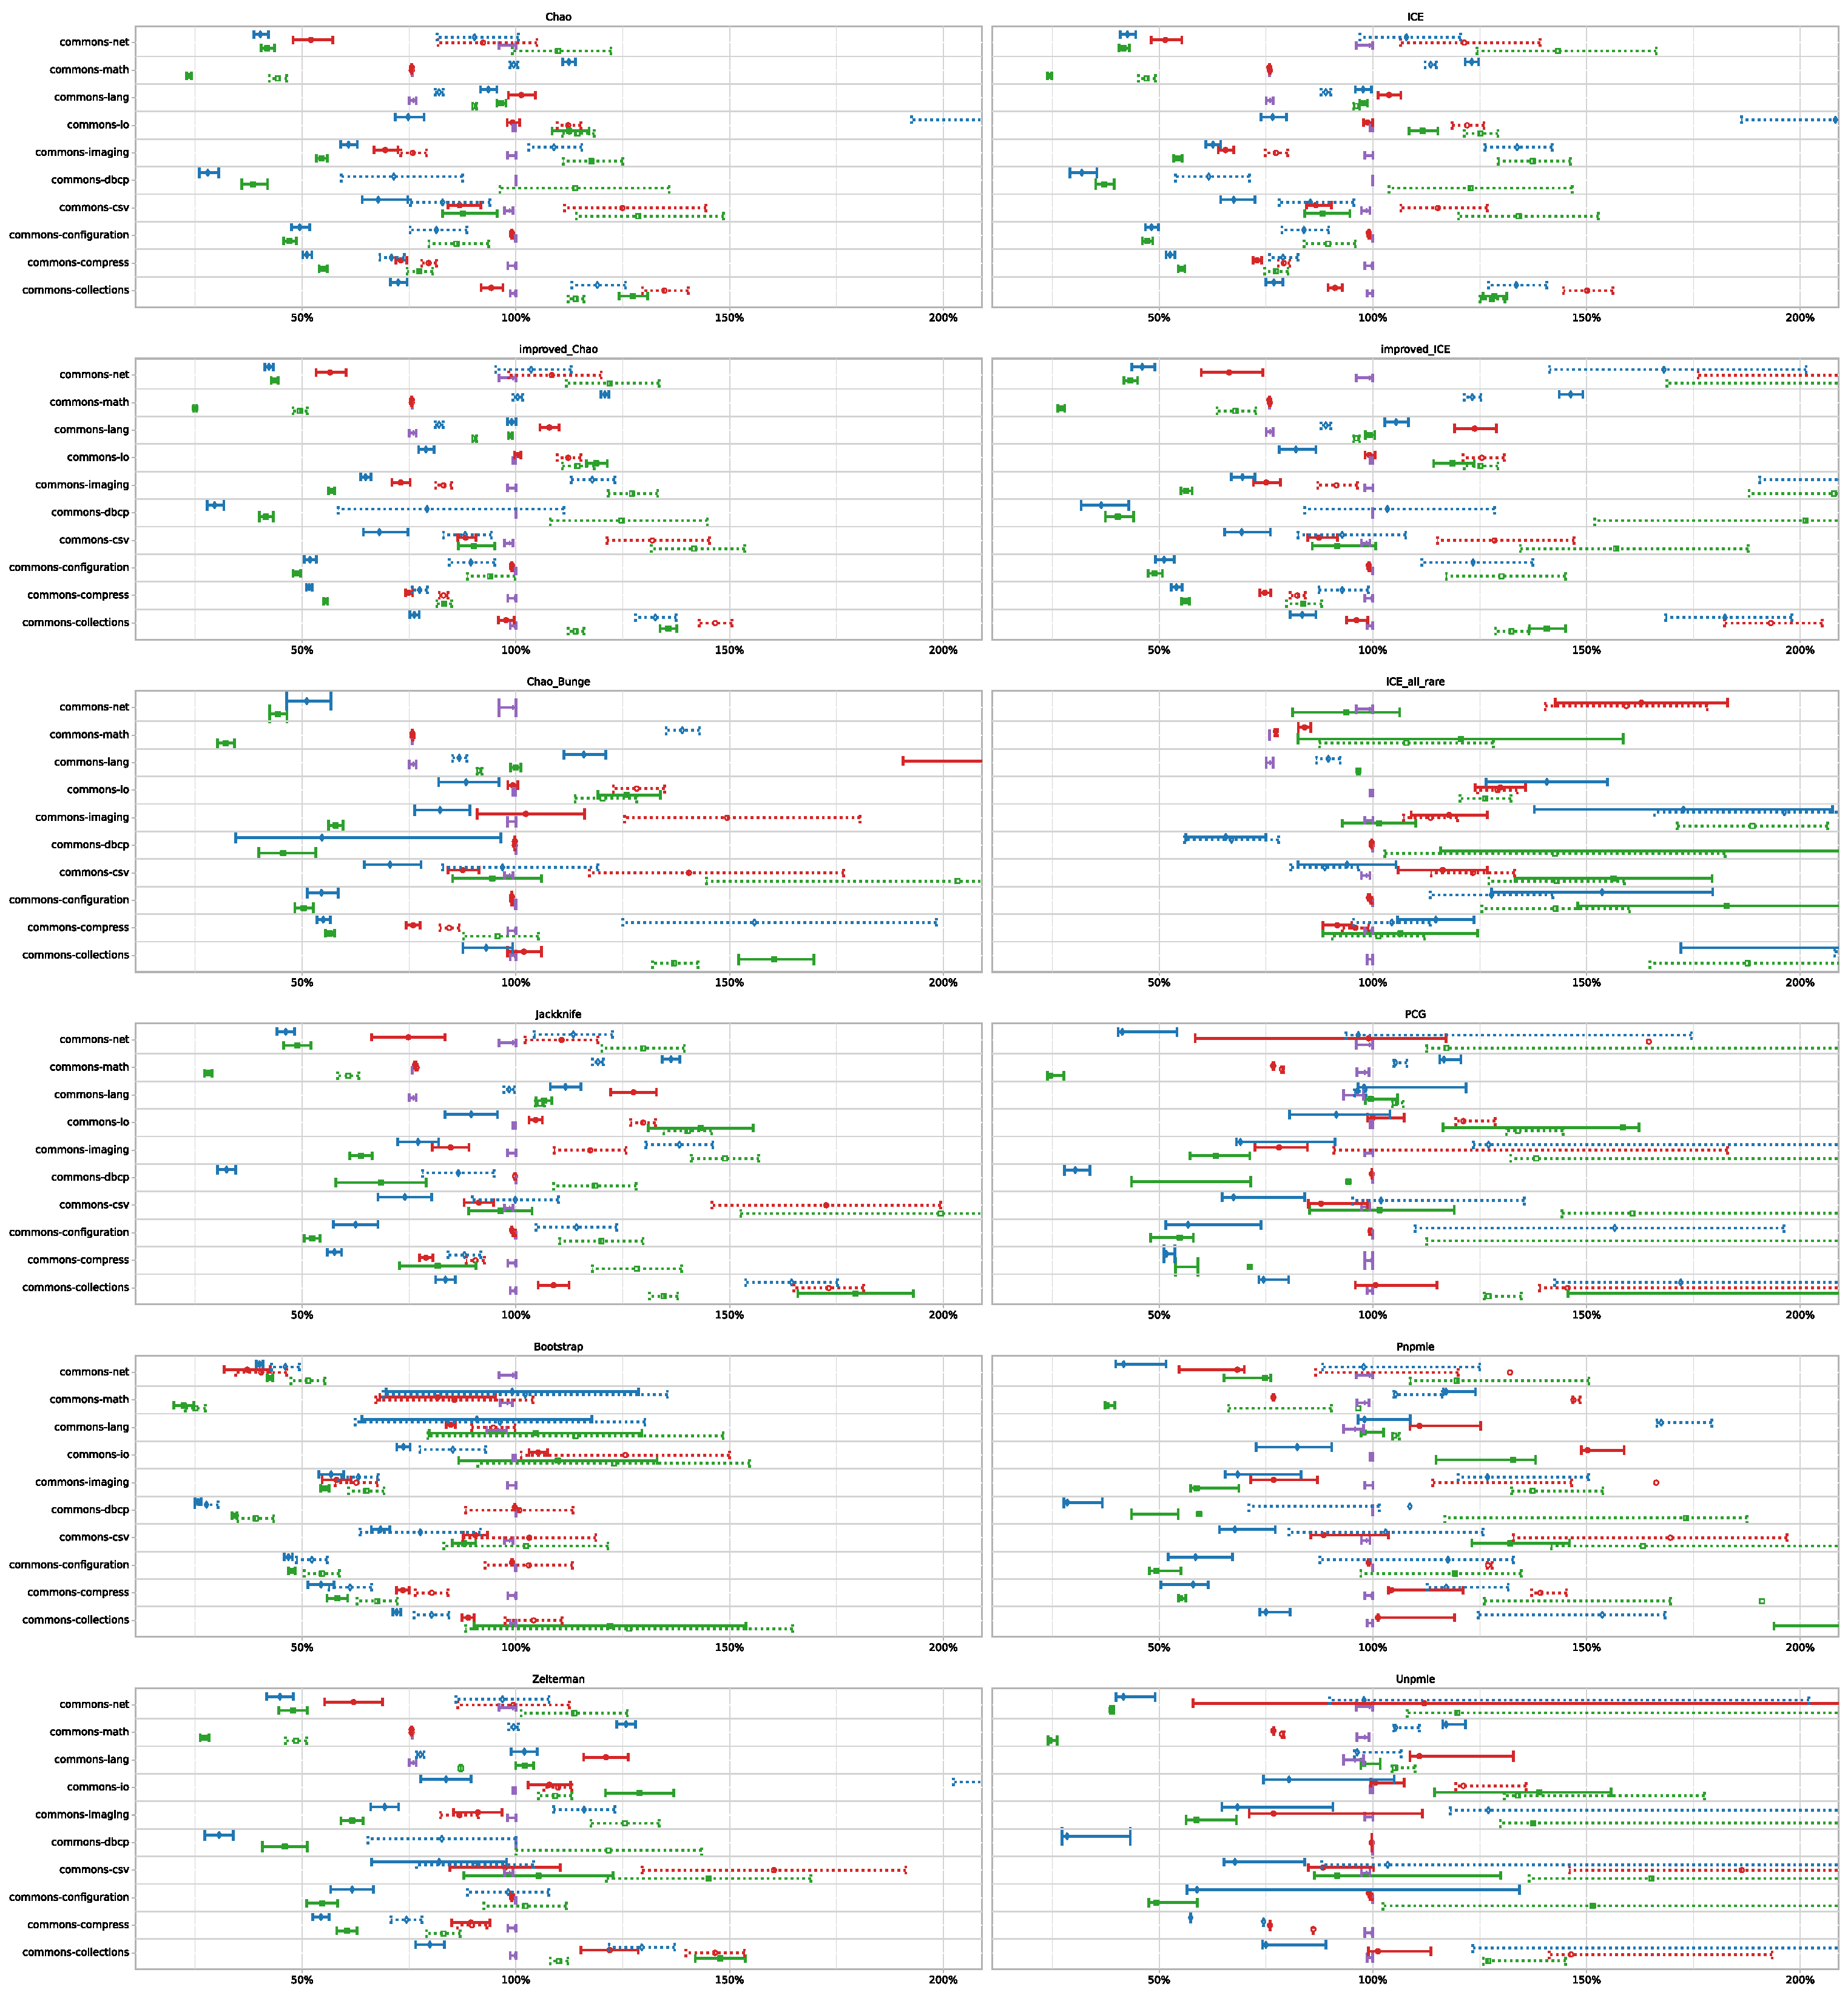
\includegraphics[width=\textwidth]{all-together.pdf}
%\caption{Killable mutants estimated by species richness estimators.
%Each plot shows the performance of a single estimator across all projects,  
%test suites (\original is red, \EvosuiteRandom is blue, and \EvosuiteDynamosa is green), and
%using class sampling (dotted lines) and method sampling (solid lines).
%For reference, estimates from manual classification are reported in solid purple.}
%\label{fig:results}
%\end{figure*}
\begin{figure*}
\begin{subfigure}{.49\textwidth}
    \centering
      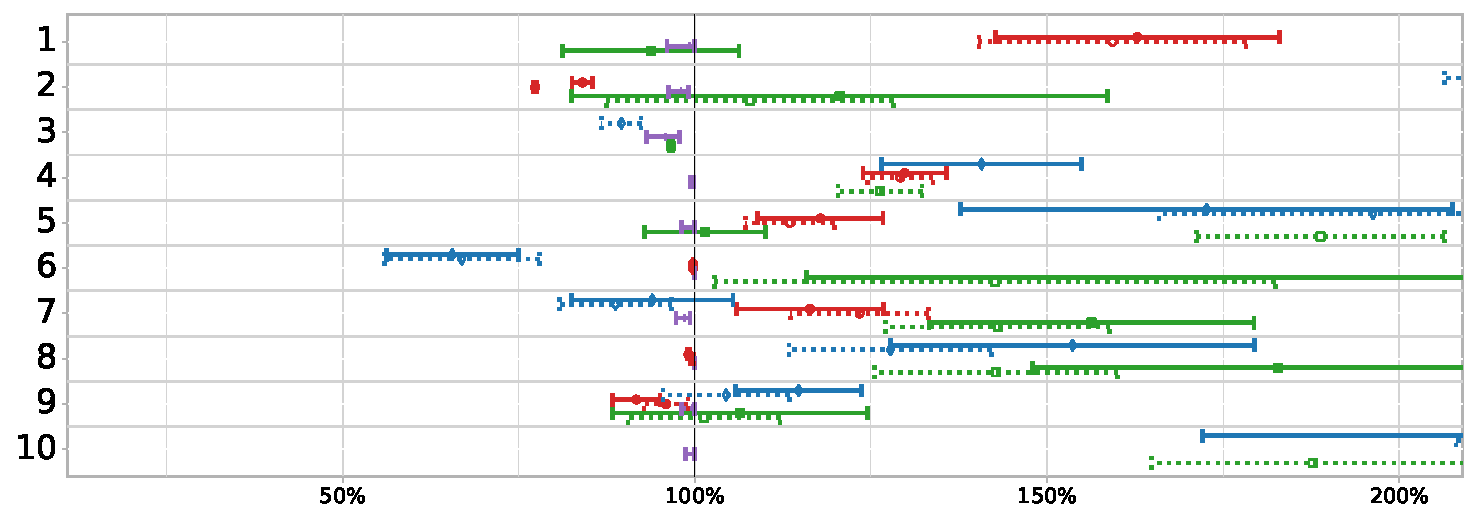
\includegraphics[width=0.95\linewidth]{charts/ggplot/estimators-no-title/ICE-k0.pdf}
\vspace*{-3mm}
\caption{\ICEallrare}
        %\caption{1b}
\end{subfigure}
\hfill
\begin{subfigure}{.49\textwidth}
    \centering
      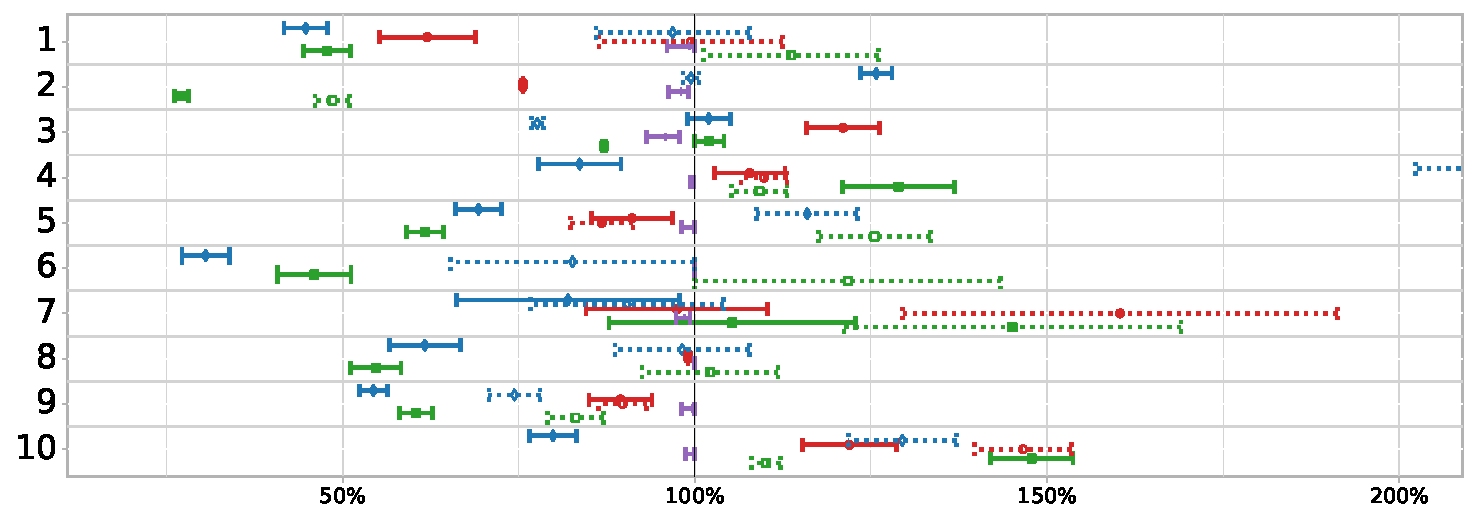
\includegraphics[width=0.95\linewidth]{charts/ggplot/estimators-no-title/Zelterman.pdf}
\vspace*{-3mm}
\caption{\Zelterman}
        %\caption{1b}
\end{subfigure}
%
\begin{subfigure}{.49\textwidth}
    \centering
      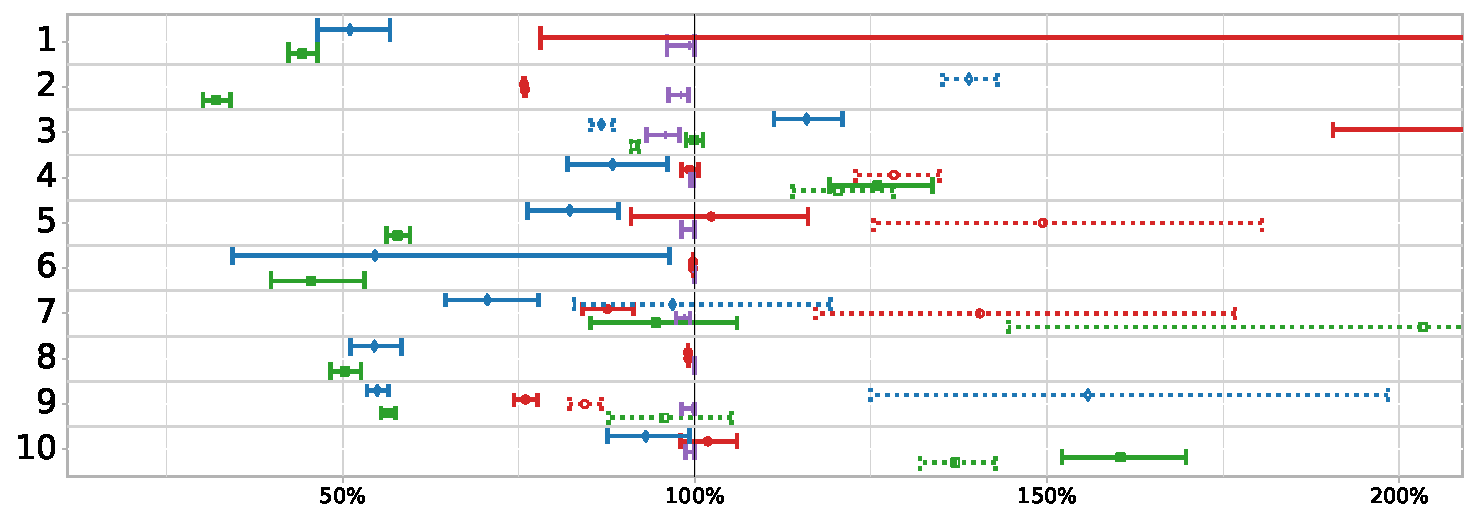
\includegraphics[width=0.95\linewidth]{charts/ggplot/estimators-no-title/Chao-Bunge.pdf}
\vspace*{-3mm}
\caption{\ChaoBunge}
        %\caption{1b}
\end{subfigure}
\begin{subfigure}{.49\textwidth}
    \centering
      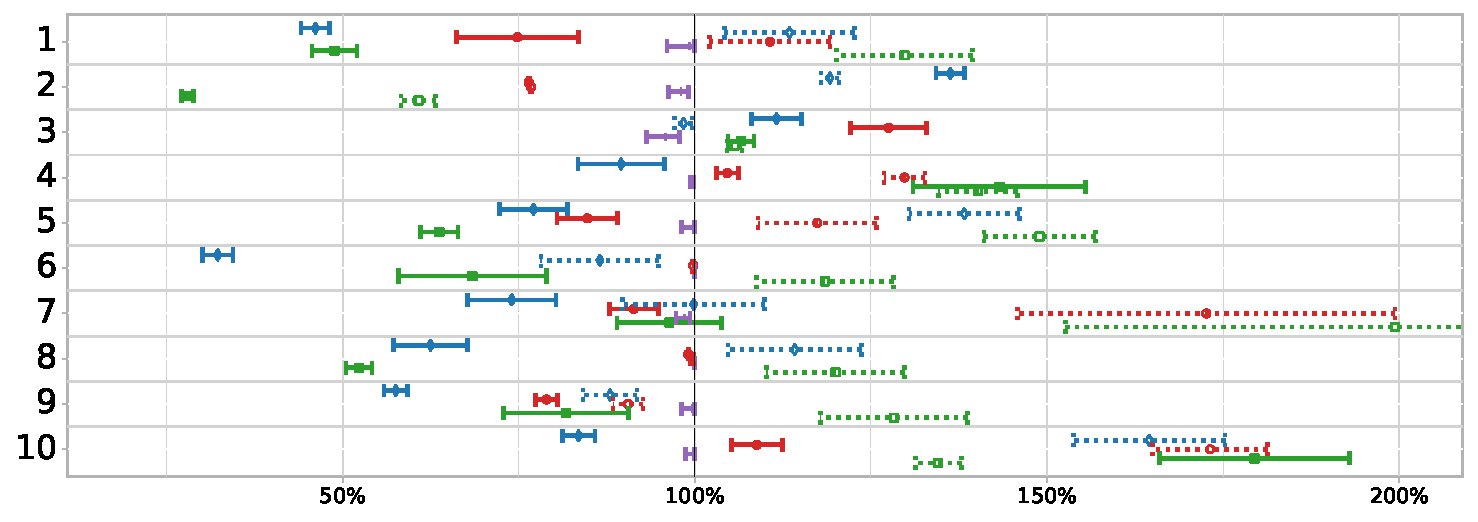
\includegraphics[width=0.95\linewidth]{charts/ggplot/estimators-no-title/Jackknife.pdf}
\vspace*{-3mm}
\caption{\Jackknife}
        %\caption{1b}
\end{subfigure}
\begin{subfigure}{.49\textwidth}
    \centering
      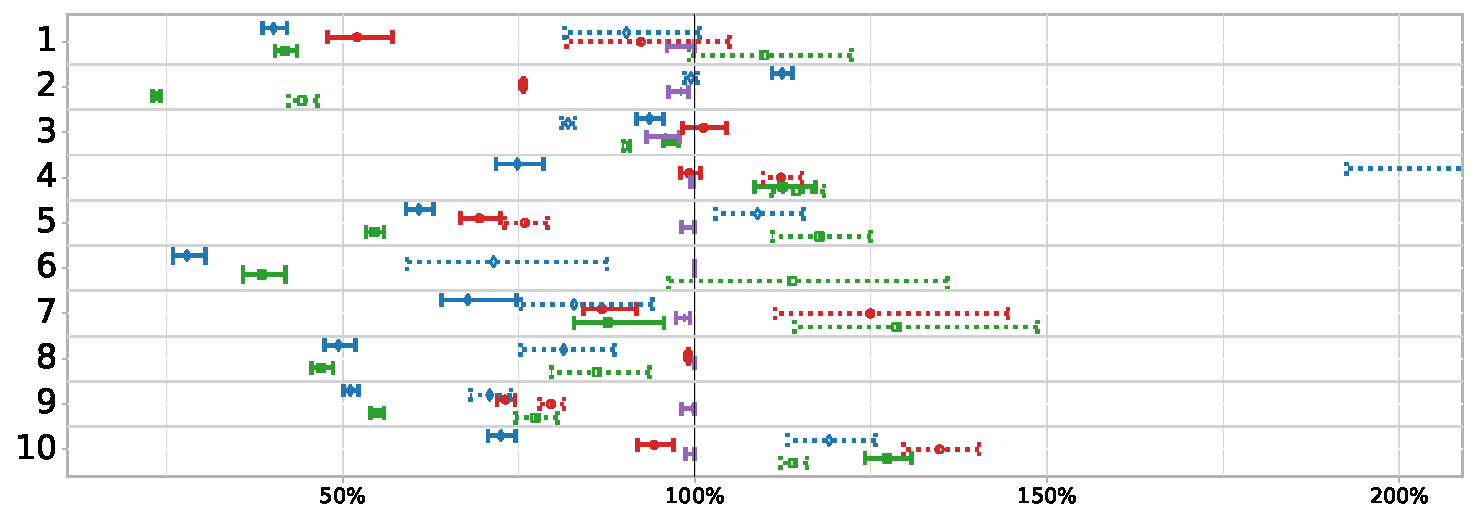
\includegraphics[width=0.95\linewidth]{charts/ggplot/estimators-no-title/Chao.pdf}
\vspace*{-3mm}
\caption{\Chao}
\end{subfigure}
\begin{subfigure}{.49\textwidth}
    \centering
      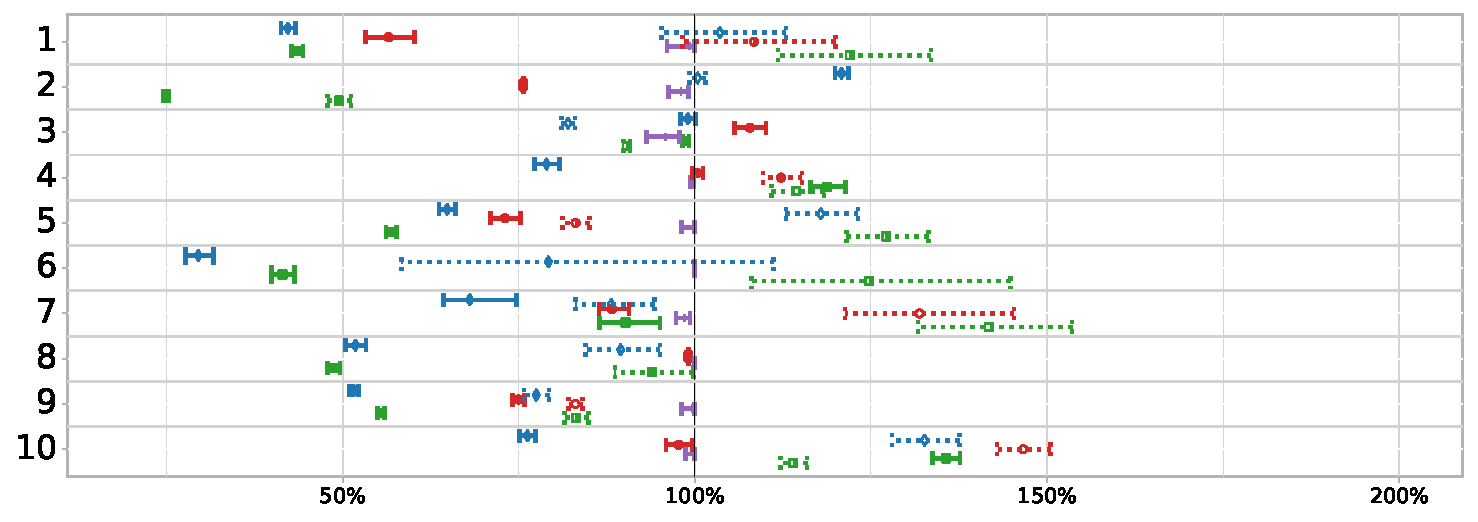
\includegraphics[width=0.95\linewidth]{charts/ggplot/estimators-no-title/iChao.pdf}
\vspace*{-3mm}
\caption{\improvedChao}
        %\caption{1b}
\end{subfigure}
\begin{subfigure}{.49\textwidth}
    \centering
      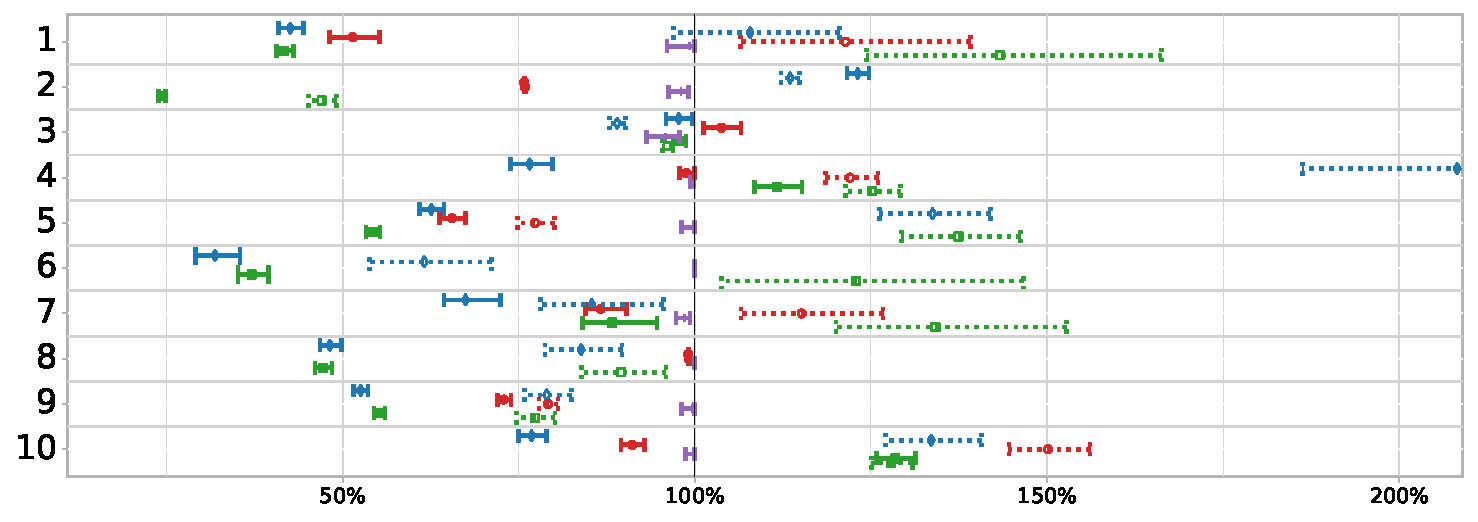
\includegraphics[width=0.95\linewidth]{charts/ggplot/estimators-no-title/ICE.pdf}
\vspace*{-3mm}
\caption{\ICE}
        %\caption{1b}
\end{subfigure}
\begin{subfigure}{.49\textwidth}
    \centering
      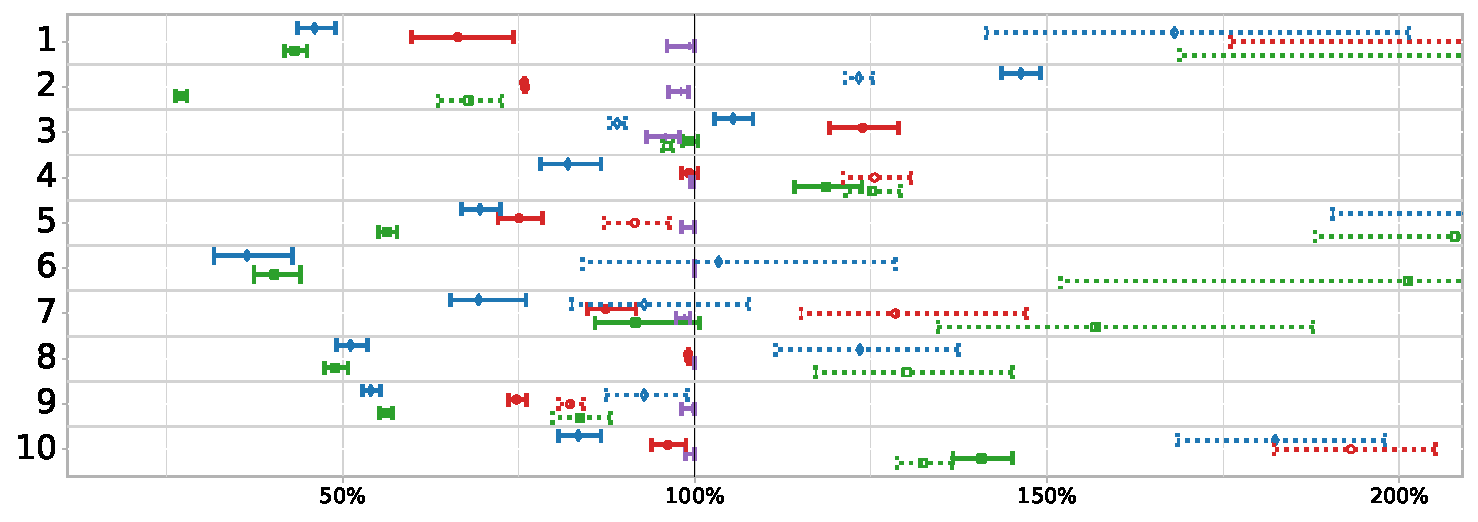
\includegraphics[width=0.95\linewidth]{charts/ggplot/estimators-no-title/ICE-1.pdf}
\vspace*{-3mm}
\caption{\improvedICE}
        %\caption{1b}
\end{subfigure}
\begin{subfigure}{.49\textwidth}
    \centering
      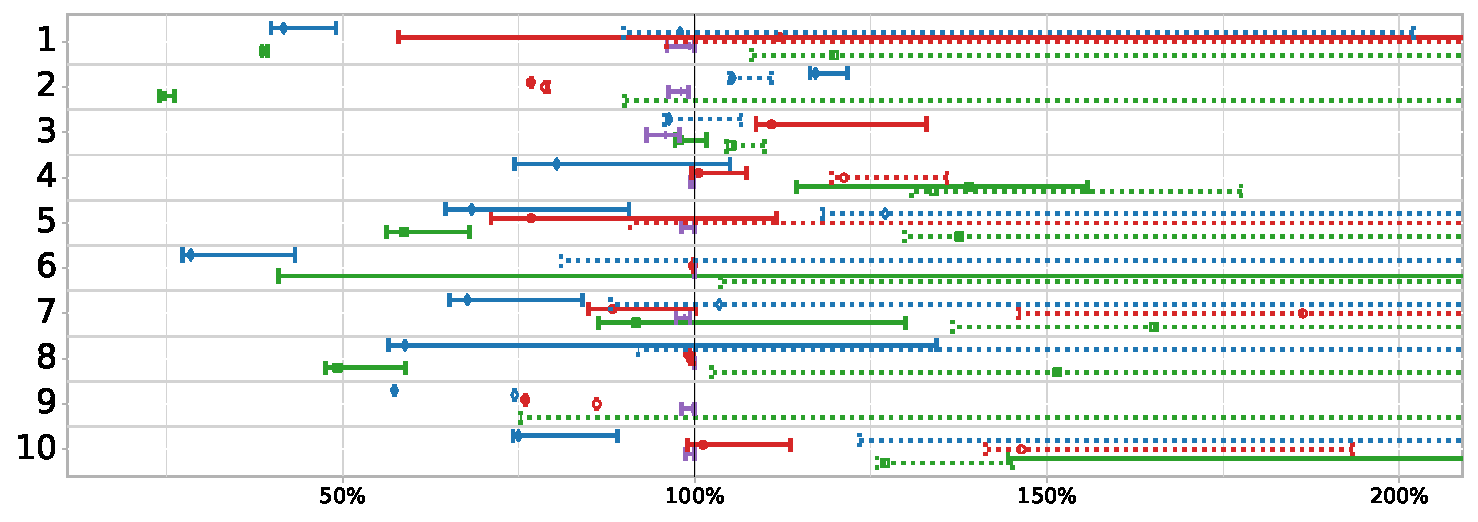
\includegraphics[width=0.95\linewidth]{charts/ggplot/estimators-no-title/Unpmle.pdf}
\vspace*{-3mm}
\caption{\Unpmle}
        %\caption{1b}
\end{subfigure}
\begin{subfigure}{.49\textwidth}
    \centering
      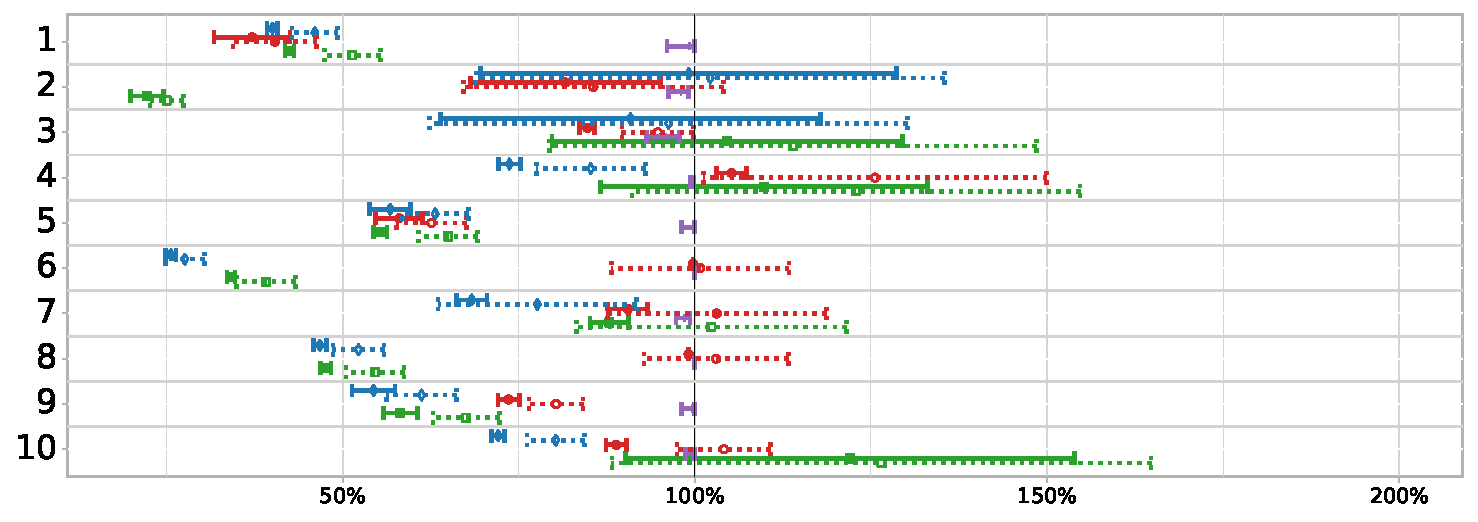
\includegraphics[width=0.95\linewidth]{charts/ggplot/estimators-no-title/Bootstrap.pdf}
\vspace*{-3mm}
\caption{\Bootstrap}
        %\caption{1b}
\end{subfigure}
\begin{subfigure}{.49\textwidth}
    \centering
      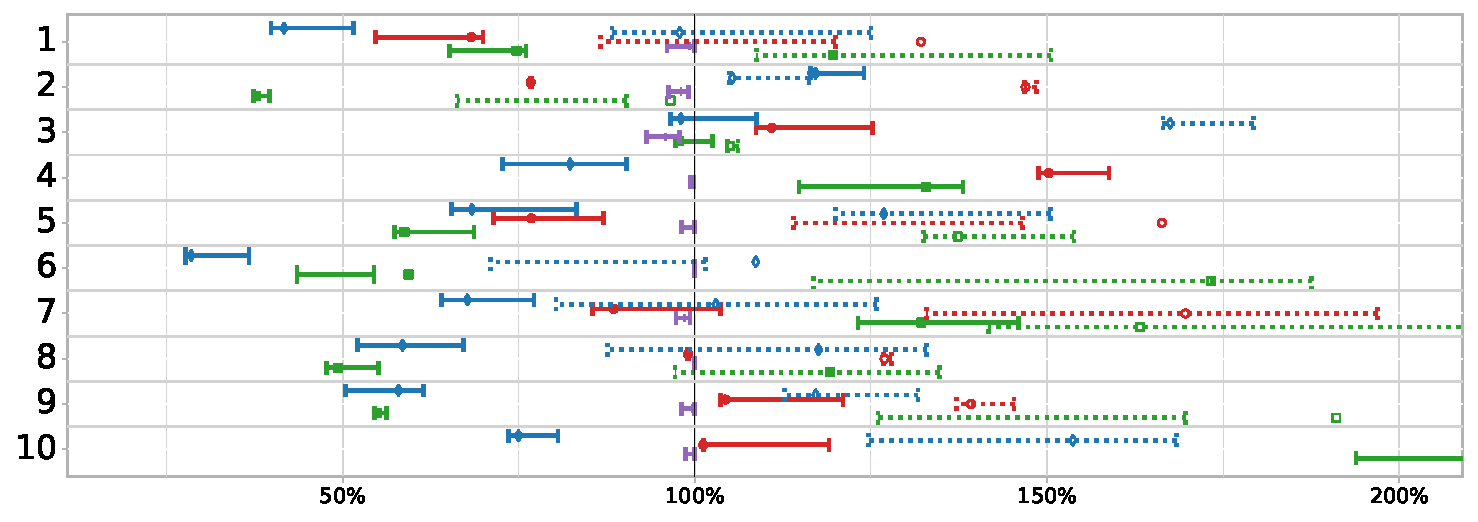
\includegraphics[width=0.95\linewidth]{charts/ggplot/estimators-no-title/Pnpmle.pdf}
\vspace*{-3mm}
\caption{\Pnpmle}
        %\caption{1b}
\end{subfigure}
\begin{subfigure}{.49\textwidth}
    \centering
      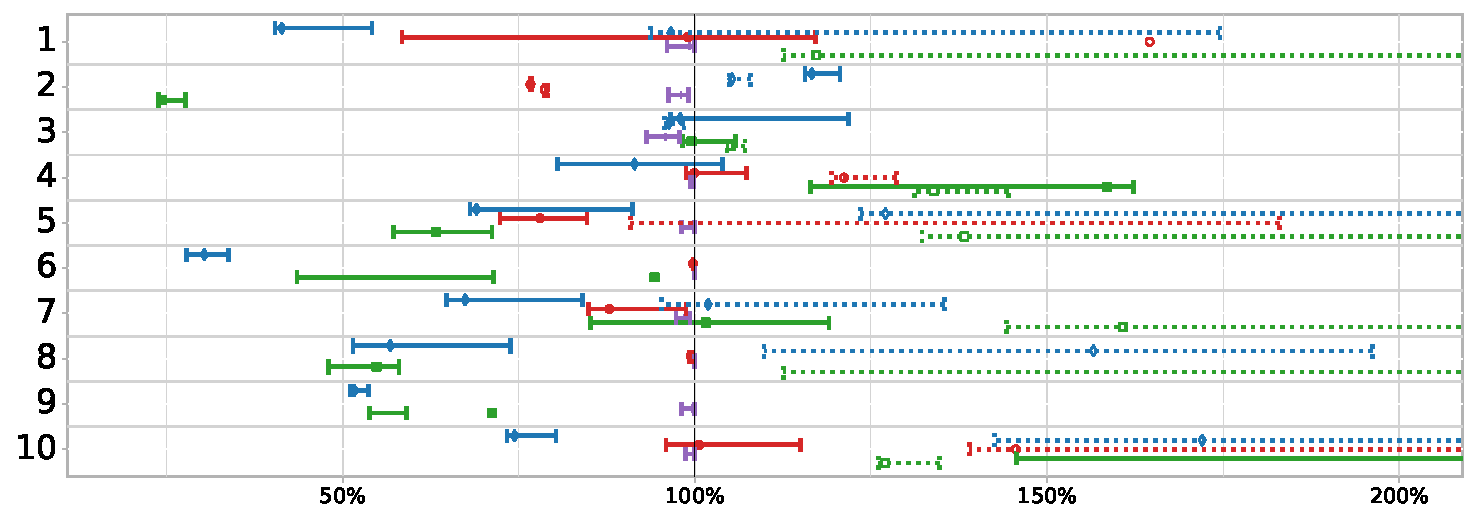
\includegraphics[width=0.95\linewidth]{charts/ggplot/estimators-no-title/PCG.pdf}
\vspace*{-3mm}
\caption{\PCG}
        %\caption{1b}
\end{subfigure}
\caption{Killable mutants estimated by species richness estimators.
Each plot shows the performance of a single estimator across all projects,  
test suites (\original is red, \EvosuiteRandom is blue, and \EvosuiteDynamosa is green), and
using class sampling (dotted lines) and method sampling (solid lines).
For reference, estimates from manual classification are reported in solid purple.
Projects (Y axis) numbered according to \Cref{tbl:subjectmeasures} column 1.
The estimates or CIs going beyond 200x of the generated mutants are not shown.}
\label{fig:results}
\end{figure*}


\bigskip

\noindent\textbf{RQ1.
What is the accuracy of frequency based estimators in predicting killable mutants?}\\
%i.e., Which statistical estimator best matches the
%estimates from manual classification 
%using manually written test suites?}\\
%
To answer this question, we considered the statistical estimators computed
using test methods for the \original test suite as sampling unit and determined
their 95\% confidence intervals. Then, we compared them against the manual
classification estimates.
%
We first checked whether the statistical estimators are significantly different
from the manual classification, i.e.,  their 95\% confidence interval did not overlap
with the 95\% confidence intervals from manual classification. Next, we computed
the difference between the two estimates using normalized mean difference (MD) computed as the
difference between the point estimate and manual classification estimate
normalized by the manual classification estimate, i.e., $\frac{E - ME}{ME}$ ($\times$
100 for percentage). We removed any estimate that resulted in negative
CI upperbound, point estimate, or no estimate at all. We also removed any
estimate that resulted in $\infty$ in upper CI. The count of such valid
estimates are given in the column \emph{Valid Estimates} in \Cref{tbl:estoriginal}.

\begin{table}
\caption{Comparison of \emph{mean difference (MD)} between method estimators
across subjects---\original test suites}
\begin{tabular}{|l|r|r|r|r|r|}
\hline

Estimator	&Valid Estimates	&CI Overlaps	&Mean	&Stdev	\\
\hline
\ICEallrare		&	8	&	0	&19.2	&	20.6\\
\Zelterman		&	9	&	1	&15.4	&	12.5\\
\ChaoBunge		&	9	&	3	&22.2	&	43.8\\
\Jackknife		&	9	&	0	&15.3	&	10.6\\
\Chao	        	&	9	&	1	&16.9	&	16.1\\
%\Chaobiascorrected	&	9	&	1	&16.9	&	16.1\\
\improvedChao		&	9	&	2	&16.0	&	14.5\\
\ICE			&	9	&	1	&18.1	&	16.1\\
\improvedICE		&	9	&	2	&16.8	&	12.8\\
\B{\Unpmle}			&	\B{10}	&	\B{5}	& \B{11.1}	&	\B{9.8}\\
\Bootstrap		&	10	&	0	&18.5	&	19.9\\
\Pnpmle			&	9	&	1	&17.8	&	16.2\\
\PCG			&	7	&	4	&8.0	&	10.2\\
\hline
\end{tabular}
\label{tbl:estoriginal}
\end{table}

Inspecting \Cref{tbl:estoriginal} reveals that in the majority of the cases the
statistical estimators were significantly different from the manual classification
and their mean absolute difference varied considerably.
%Out of \projectCount test subjects,
\Unpmle behaved the most consistently with manual classification
achieving 50\% agreement (five out of \projectCount test subjects,
MD $11.1$\%, Stdev. 9.8\%.) However, we note that the confidence
intervals were very large in many cases for \Unpmle (\Cref{fig:results}).
%PCG was next nearest with a CI overlap 4~times with manual classification
%estimate.
%
%
%ALESSIO:  what <5 means here?
The other estimators were significantly different % ($<5$)
(less than $5$ CI overlaps)
 than manual classification.

\begin{tcolorbox}[boxrule=0.5pt, arc=4pt, boxsep=0pt, width=\columnwidth]
There is a statistically significant difference between the estimates
from \original test suites and manual classification for
every estimator examined.
\end{tcolorbox}

\noindent\textbf{RQ2.
%Which statistical estimator best predicts the estimates
%from manual classification when given unbiased test suites?
Are frequency based estimators affected by sampling strategies?}\\
%
To answer this question, we considered the statistical estimators computed
using test methods for \EvosuiteRandom and \EvosuiteDynamosa test suites as sampling unit
and determined their 95\% confidence intervals.
%
Next, we checked whether the estimators' 95\% confidence intervals consistently
overlapped with the one from manual classification, and computed their mean absolute
difference with respect to manual classification.
%
The results are given in \Cref{tbl:estrandom} for \EvosuiteRandom, and in
\Cref{tbl:estdynamosa} for \EvosuiteDynamosa (and \Cref{tbl:estoriginal} for \original).


\begin{table}
\caption{Comparison of \emph{mean difference (MD)} between method
estimators across subjects---\EvosuiteRandom test suites}
\begin{tabular}{|l|r|r|r|r|r|}
\hline
Estimator	&Valid Estimates	&CI Overlaps	&Mean	&Stdev	\\
\hline
\ICEallrare	&	9	&	1	&81.2	&	71.3\\
\B{\Zelterman}	&	\B{10}	&	\B{1}	&\B{32.6}	&	\B{19.6}\\
\ChaoBunge	&	10	&	1	&42.5	&	42.6\\
\Jackknife	&	10	&	0	&33.1	&	18.3\\
\Chao	&	10	&	1	&37.1	&	21.2\\
%\Chaobiascorrected	&	10	&	1	&37.1	&	21.2\\
\improvedChao	&	10	&	0	&36.1	&	20.0\\
\ICE	&	10	&	1	&36.7	&	19.6\\
\improvedICE	&	10	&	0	&36.5	&	18.2\\
\Unpmle	&	9	&	2	&37.8	&	17.7\\
\Bootstrap	&	10	&	2	&36.7	&	23.1\\
\Pnpmle	&	10	&	1	&34.0	&	20.2\\
\PCG	&	10	&	2	&33.7	&	21.4\\
\hline
\end{tabular}
\label{tbl:estrandom}
\end{table}
%
\begin{table}
\caption{Comparison of \emph{mean difference (MD)} between method
estimators across subjects---\EvosuiteDynamosa test suites}
\begin{tabular}{|l|r|r|r|r|r|}
\hline
Estimator	&Valid Estimates	&CI Overlaps	&Mean	&Stdev	\\
\hline
\ICEallrare	&	9	&	4	&77.9	&	77.5\\
\Zelterman	&	10	&	1	&39.2	&	20.6\\
\ChaoBunge	&	10	&	1	&40.8	&	22.3\\
\Jackknife	&	10	&	1	&39.3	&	24.9\\
\Chao	&	10	&	1	&39.1	&	24.9\\
%\Chaobiascorrected	&	10	&	1	&39.1	&	24.9\\
\improvedChao	&	10	&	0	&39.5	&	23.0\\
\ICE	&	10	&	1	&39.2	&	24.8\\
\improvedICE	&	10	&	1	&39.8	&	22.9\\
\Unpmle	&	7	&	2	&39.5	&	26.8\\
\B{\Bootstrap}	&	\B{10}	&	\B{3}	&\B{39.1}	&	\B{24.8}\\
\Pnpmle	&	10	&	1	&49.5	&	42.6\\
\PCG	&	9	&	1	&42.4	&	40.0\\
\hline
\end{tabular}
\label{tbl:estdynamosa}
\end{table}
%

A comparison reveals that the overlaps between confidence intervals
from manual classification and \EvosuiteRandom (\Cref{tbl:estrandom}) was
considerably fewer than that between manual and \original (\Cref{tbl:estoriginal}).
The smallest difference in MD was observed for \Zelterman
(mean 32.6\%, Stdev. 19.6\%).
%
For \EvosuiteDynamosa, the situation was slightly better (\Cref{tbl:estdynamosa}), \ICEallrare
overlapped with manual classification estimates 4 times out of 10.
The smallest difference in MD, with least variation was observed for
Bootstrap (mean 39.1\% Stdev. 24.8\%).

Comparing the estimators across \EvosuiteRandom and \EvosuiteDynamosa
test suites, we also observed that none behaved consistently, i.e.,
their 95\% confidence intervals almost never overlapped.

\begin{tcolorbox}[boxrule=0.5pt, arc=4pt, boxsep=0pt, width=\columnwidth]
The difference between estimates from \EvosuiteRandom and \EvosuiteDynamosa
to the estimates from manual classification is statistically significant for every estimator examined.
Likewise, estimates from \EvosuiteRandom are always significantly differently
than the ones from \EvosuiteDynamosa.
\end{tcolorbox}



\noindent\textbf{RQ3. 
%Which mapping of sampling units best predicts the estimates from manual classification?
Are frequency based estimators affected by sampling units?
}\\ % when given unbiased test suites from \Evosuite?}
To answer this question, we compared the estimations 
using test methods as sampling units to estimations using test classes as
sampling units for all tests suites and
determined their 95\% confidence intervals.
%
Next, we checked whether the estimators' 95\% confidence intervals consistently
overlapped with the one from manual classification, and computed their mean absolute
difference with respect to manual classification.
%
The results are given in tables \Cref{tbl:estoriginalclass},
\Cref{tbl:estrandomclass}, and \Cref{tbl:estdynamosaclass}.
These results are also plotted as dotted lines in \Cref{fig:results}.

\begin{table}[t]
\caption{Comparison of \emph{mean difference (MD)} between class
estimators across subjects---\original test suites}
\begin{tabular}{|l|r|r|r|r|r|}
\hline
Estimator	&Valid Estimates	&CI Overlaps	&Mean	&Stdev	\\
\hline
\ICEallrare	&	9	&	1	&35.2	&	51.4\\
\Zelterman	&	9	&	1	&36.7	&	51.8\\
\ChaoBunge	&	7	&	0	&22.8	&	19.1\\
\Jackknife	&	10	&	0	&41.2	&	53.5\\
\Chao	&	9	&	1	&32.4	&	42.5\\
%\Chaobiascorrected	&	9	&	1	&32.4	&	42.5\\
\improvedChao	&	9	&	1	&35.9	&	49.5\\
\ICE	&	9	&	0	&41.2	&	57.9\\
\improvedICE	&	8	&	0	&40.2	&	43.5\\
\Unpmle	&	6	&	0	&31.9	&	31.8\\
\B{\Bootstrap}	&	\B{10}	&	\B{6}	&\B{16.9}	&	\B{19.2}\\
\Pnpmle	&	8	&	1	&64.9	&	34.8\\
\PCG	&	6	&	1	&43.9	&	39.5\\
\hline
\end{tabular}
\label{tbl:estoriginalclass}
\end{table}
%
\begin{table}[t]
\caption{Comparison of \emph{mean difference (MD)} between class
estimators across subjects---\EvosuiteRandom test suites}
\begin{tabular}{|l|r|r|r|r|r|}
\hline
Estimator	&Valid Estimates	&CI Overlaps	&Mean	&Stdev	\\
\hline
\ICEallrare	&	8	&	1	&61.1	&	65.1\\
\Zelterman	&	10	&	4	&25.4	&	39.0\\
\ChaoBunge	&	4	&	1	&27.3	&	26.0\\
\Jackknife	&	10	&	2	&33.1	&	44.7\\
\Chao	&	10	&	2	&26.3	&	33.3\\
%\Chaobiascorrected	&	10	&	2	&26.3	&	33.0\\
\improvedChao	&	10	&	2	&27.7	&	40.7\\
\ICE	&	10	&	1	&29.7	&	29.9\\
\improvedICE	&	10	&	3	&52.4	&	61.1\\
\Unpmle	&	7	&	3	&34.9	&	63.9\\
\Bootstrap	&	10	&	2	&30.9	&	23.0\\
\B{\Pnpmle}	&	\B{9}	&	\B{4}	&\B{23.6}	&	\B{24.9}\\
\PCG	&	7	&	3	&24.3	&	29.2\\
\hline
\end{tabular}
\label{tbl:estrandomclass}
\end{table}
%
\begin{table}[t]
\caption{Comparison of \emph{mean difference (MD)} between class
estimators across subjects---\EvosuiteDynamosa test suites}
\begin{tabular}{|l|r|r|r|r|r|}
\hline
Estimator	&Valid Estimates	&CI Overlaps	&Mean	&Stdev	\\
\hline
\ICEallrare	&	10	&	3	&49.3	&	46.4\\
\Zelterman	&	10	&	1	&20.7	&	16.3\\
\ChaoBunge	&	5	&	1	&34.6	&	42.4\\
\Jackknife	&	10	&	0	&37.3	&	25.6\\
\B{\Chao}	&	\B{10}	&	\B{2}	&\B{19.9}	&	\B{14.0}\\
%\Chaobiascorrected	&	10	&	2	&19.7	&	14.0\\
\improvedChao	&	10	&	0	&22.5	&	14.6\\
\ICE	&	10	&	1	&28.0	&	15.4\\
\improvedICE	&	10	&	1	&52.4	&	42.4\\
\Unpmle	&	7	&	0	&35.5	&	19.4\\
\Bootstrap	&	10	&	4	&36.9	&	20.9\\
\Pnpmle	&	10	&	1	&55.7	&	44.5\\
\PCG	&	8	&	0	&57.7	&	51.7\\
\hline
\end{tabular}
\label{tbl:estdynamosaclass}
\end{table}


From \Cref{tbl:estoriginalclass}, we see that Bootstrap had the best
overlap with CI (6 times), and mean difference (mean 16.9\%, Stdev. 19.2\%).
%
For \EvosuiteRandom and \EvosuiteDynamosa, the situation was the same as before
with the manual classification and estimates confidence intervals not
overlapping a majority of the time.
%
Furthermore, we also found that the estimates from method level sampling units
and class level sampling units are also statistically significantly different.

\begin{tcolorbox}[boxrule=0.5pt, arc=4pt, boxsep=0pt, width=\columnwidth]
The difference between estimates from test method and test class level
estimators to the estimates from manual classification are statistically
significant for every estimator examined. Furthermore, the difference between
each other is statistically significant for every estimator examined.
\end{tcolorbox}


\subsection{What Does This Mean in Practice?}

We note that some of the estimators seem to have come close to the manual
estimates some of the time. However, one of the dangers in relying on numerous
statistical comparisons is that there may be statistical artifacts in the data,
which may not correspond to the characteristics of the original population.
To mitigate the impact of such artifacts, before starting the project, we
decided that we will only consider those instances where estimators were
able to consistently achieve reasonable results across at least a majority of
the projects.

%we have intentionally avoided investigating why certain estimators seem to have
%worked in certain specific projects some of the time.


Given that using various test suites and sampling strategies always produced
inconsistent and unsatisfactory results for all the considered estimators
even though the underlying sampled quantity, i.e., killable mutants, did not
change, our (current) conclusion is that frequency based statistical %standard species richness 
estimators are unsuitable for estimating killable mutants.

Our negative results
% from applying species richness estimators to mutation analysis
suggest a need of further empirical evidence and additional analysis
% are
%needed
to understand the impact of various assumptions made by those %species richness 
estimators and their applicability to mutation analysis.
% whether and how good the 
%hold when estimating equivalent mutants. 
%
%In other words, despite the progress in using those estimators to assess residual risk 
%from the structural coverage point of view, for mutation analysis we are not there yet!

%Nonetheless, our recommendation to the testers
%is to continue to rely on sampling live mutants for estimating
%the number of killable mutants within the required confidence interval,

%Given the dismal performance of STADS on estimating the number of killable
%mutants, we believe that further empirical evidence and detailed analysis is 
%needed to understand various assumptions made by species diversity models, and
%whether they are applicable to specific domains before they can be reliably
%used by the practitioners.




%
%class level sampling units are predicting the same quantity as that of the method level sampling
%units, this suggests the only remaining possibility. That the statistical estimation 



%One of the uses of mutation analysis is that it can be used to estimate the
%residual defect density~\cite{fuzzingbook2022:MutationAnalysis}, i.e., 
%an accurate estimate of the remaining live mutants can provide
%insights on the bugs that remains to be found.

%The STADS~\cite{bohme2018stads}
%framework, which relies on the same species richness estimates that we studied here
%
% to provide accurate estimates on residual defect density.


%Beyond mutation analysis, ours is also one of the first studies that evaluates
%the STADS framework~\cite{bohme2018stads} for estimation. A comprehensive
%evaluation in other fields such as residual defect estimation is difficult as
%it is very hard to get the ground truth on the number of defects a large
%program may still contain. Mutation analysis is a useful test bed for STADS
%because we have an upper bound on the number of killable mutants -- the total
%number of mutants generated. However, we note that in many cases, the estimated
%number of killable mutants from class level estimators
%(including the error bars) lie beyond the total number of mutants generated.
%Given the dismal performance of STADS on estimating the number of killable
%mutants, we believe that further empirical evidence and detailed analysis is 
%needed to understand various assumptions made by species diversity models, and
%whether they are applicable to specific domains before they can be reliably
%used by the practitioners.





\subsection{Threats to Validity}

\noindent\textbf{External Validity.}
Our study was conducted on a limited number of programs from a specific
open-source repository and using a small number of test producers;
hence, our findings
may not generalize to other projects and test suites produced by other means.
 %other strategies (e.g., model-based, single object genetic algorithm)
%
To reduce this risk, we selected multiple projects from Apache Commons and
used EvoSuite in two exemplary configurations.
%
Apache Commons projects are popular, implement different functionalities, and
%and are developed  according to community-set practices by independent development teams.
%Hence, they 
are comparable to % generally compared to seen to have similar quality as in 
well run industrial projects.
%, and form components in many such systems.
EvoSuite, instead, implements standard baselines %(e.g., random) 
and
well established and effective algorithms %(e.g., DynaMOSA), 
that generate test suites with remarkably different features.
%s
We use a single run of both the test generator (randomized) on our classes.
%
While multiple runs are required for statistical confidence of the results,
we note that our approach is similar to the one adopted by established biometrics
studies that draw conclusions from single sampling campaigns.

\noindent\textbf{Internal Validity.}
The test suites automatically generated did not always achieve high coverage, 
hence, they can lead to larger uncertainty in the final estimation of equivalent mutants. 
However, we note that this situation is similar to the one currently faced by software practitioner. % has to contend with.
%
Next, our analysis can be subject to bugs, sampling errors, and mutant mis-classifications
that might bias our results.
%
For instance, the test generator could not generate unit tests for all the classes under analysis,
hence failing to sample their mutants.
We tried to mitigate this risk by reviewing the code of JUGE and our scripts, 
cross-checking the results, and use the largest possible subset of classes for which
test generation succeeded.
It is possible that our manual classification is biased. We tried to mitigate it by cross-checking between three classifiers.
%Specifically, We could use only a (largest possible) subset of classes for test generation as
%some of the classes resulted in hanging or crashes of test generators. 

\noindent\textbf{Construct Validity.} We are the first to apply
frequency based statistical models %species richness 
to the problem of killable mutants estimation; hence, 
our mapping of statistical estimators to the mutation testing domain
%may be non-optimal and 
might not to capture important variables. %We also acknowledge this threat.
%
We tried to mitigate this threat by adopting different sampling strategies.
% Conclusions validity maybe?
%Are the species diversity estimators
%applicable to mutation analysis? That is, are there assumptions that mutation
%analysis data violates, that makes these estimators inapplicable?
%We acknowledge this threat. The mitigation is that, even if there are
%assumptions that are unfulfilled, the estimators are invented such that they
%are robust to limited relaxations in assumptions. 
%




\section{Related Work}
%\subsection{Equivalent Mutant Classification}
%\begin{table}
%  \caption{Previous studies for manual classification and the number of cross-validating researchers}
%  \begin{tabular}{|l|r|r|r| }
%    \hline
%    Author(s) & Year & Studied Eqv. & \# Researchers \\
%    \hline
%    Acree~\cite{acree1980mutation} & 1980 & 90 & 3 \\
%    Schuler et al.~\cite{schuler2013covering} & 2013 & 140 & 1 \\
%    Just et al.~\cite{just2013using} & 2013 & 17 & 1 \\
%    Yao et al.~\cite{yao2014a} & 2014 & 1230 & 1 \\
%    \textbf{This paper} & 2020 & 1016 & 3 \\
%    \hline
%  \end{tabular}
%  \label{tbl:eqvresearch}
%\end{table}
Mutation analysis is considered a primary way of evaluating test quality~\cite{papadakis2019mutation};
thus, mutation score is usually considered as a test suite adequacy metrics~\cite{just2014are,andrews2005is,andrews2006using,daran1996software}. 
%The complement of mutation score was also found to be instrumental in characterizing
%residual faults~\cite{ahmed2016can}. 
Unfortunately, equivalent mutants have vexed practitioners from the very beginning~\cite{budd1982two},
and remains an open issue~\cite{madeyski2014overcoming} that affects also residual risk estimation.
%
To address this issue, we proposed to estimate killable mutants using
frequency based statistical estimators that have been applied recently to 
estimate reachable coverage
%species richness estimators 
and conducted a large empirical study that included
$10$ mature open-source Java projects, $3$ types of test suites, and the 
manual classification of $1016$ live mutants involving $3$ researchers.

A few previous studies also relied on the manual mutants classification.
% of equivalent mutants.
%(see \Cref{tbl:eqvresearch}).
% summarizes our and those studies' 
%manual classification of equivalent mutants,  the
%publication year, number of mutants classified, and number of
%researchers that cross validated the classifications 
%
Acree's study~\cite{acree1980mutation} 
%was the first researcher to classify equivalent mutants manually.
%For his study, Acree  classified mutants by leveraing 
involved two competent software engineers experts in mutation analysis
that classified
live mutants from four COBOL programs.
%with experience in development of mutation analysis systems
%but without exposure to the programs under analysis,
%and classified mutants from four COBOL programs.
%(For the two programs were information is given, they are approximately 150 LOC in size),
Similar to our study, Acree used manually written tests
% set designed to cover the major points of the specification
%was used 
for eliminating a large chuck of mutants; however, differently 
from us, the labelers had no exposure to the programs under analysis and
focused on small COBOL programs.
%most, but not all detectable mutants,
%whereas, after the classification, the collected answers were
%compared against a reference prepared by the author.
%---that is, the obvious (easily detectable)
%non-equivalent mutants were eliminated but the non-obvious ones that were
%harder to kill were left in. A human tester manually generated tests to cover
%the major points of specification, and trying to kill all the mutants.
%
%The mutants were chosen from four COBOL programs (For the
%two programs were information is given, they are approximately 150 LOC in size),
%and the subjects were asked to mark each mutant as equivalent or
%non-equivalent with no time limit. Answers were compared against a reference
%prepared by the author.
During his study, Acree documented various misclassifications (avg. 23\%),
suggesting that even manual classification has errors. 
%
We also found misclassifications (see \Cref{tbl:classified}, \emph{Misclass.} column),
but achieved better accuracy~(less than $5\%$ misclassifications on avg),\footnote{This measure does not consider the results of \texttt{commons-csv} that we used for training the labelers.}
%, for which the misclassification rate is comparable.}
arguably because we trained the labelers
% before the study, gave them access to the original program,
and followed a structured and systematic classification protocol.
%Finally, we used the services of two researchers as classifiers, and resolved
%conflicts using a third. We believe that this procedure makes our procedure
%systematic and less error prone.

%however, compared to Acree's study, on average we observed a drastically smaller
%rate (less than $5\%$).\footnote{This does not consider the results of commons-csv used for training the labelers, for which the misclassification rate is comparable.}
%We argue that this improved classification accuracy resulted from 
%training the labelers and employing a more structured classification protocol.
%, having access to the program under tests, and employing an expert researcher to oversee the entire process.
% errors, i.e.,  non-equivalent mutant is classified as equivalent and vice-versa,
%Type I error, when a non-equivalent mutant is classified as equivalent,
%and Type II error, when an equivalent mutant is classified as non-equivalent.
%%
%Type I error for subject 1 was 14.3\% while for subject 2 it was 11.1\% of the
%total non-equivalent mutants. Type II error for subject 1 was 31.5\% while
%for subject 2 it was 35.1\% of the equivalent mutants\footnote{Note that one
%is based on equivalent while other is based on non-equivalent.}. The study by
%Acree suggests that even manual classification may not be error free. 
%
%
%
% 6 person months from a
Other studies of note are by Yao et al.~\cite{yao2014a} on $18$ C programs,
and Gr\"un et al.~\cite{grun2009impact} (extended by Schuler et al.~\cite{schuler2010covering})
on $7$ Java programs.
%
Both studies involved a single researcher but classified a different amount of live mutants,
$1,194$  Yao et al. and %drastically few (i.e., $140$) Gr\"un et al.
$140$ Gr\"un et al.
%
Yao et al.'s study 
%used the original (system) test suites to identify live mutants, 
estimated that 77\% of all mutants are killable, while Gr\"un et al.'s reported that 
45\% of the \emph{classified} live mutants are equivalent.
%
Unfortunately, none of those studies reported the misclassification rate.
%Out of those analyzed (which were non-killed mutants after the original test suite were run, 23\% was found equivalent.)
%Unfortunately, no classification error rate is available as only a single researcher was
%involved in Yao et al.'s study.
% the confidence is high when a mutant is marked as non-equivalent, as it is
% accompanied by a test case.
Compared to those studies, 
our manual classification required (modulo the number of mutants) the same amount of time, 
but involved twice as many researchers. We also considered real-world, more complex, and arguably more
difficult to evaluate, projects, and a sufficiently representative set of mutation operators~\cite{gopinath2017mutation}.
%further do not restrict our research to a selected set of mutants, which was shown previously to be problematic~\cite{gopinath2017mutation}, and considered both m
Finally, we studied manually written and automatically generated unit test suites, 
that covered more mutants and resulted in estimating a higher number (generally above 90\%) of killable mutants.

Papadakis et al.~\cite{papadakis2014mitigating} is a study similar to ours,
with more numerous subjects. However, compared to that study,
we consider larger programs and different test suites, do not employ selective mutation, whose limits have been discussed empirically and theoretically~\cite{gopinath2017mutation,gopinath2016on}, and we employ mechanisms such as conflict identification and resolution, to reduce manual classification error proneness. %Furthermore, test suite size can be misleading and one should be careful to use it (Chen 2020).
We also note that Papadakis et al. requires manual classification, however limited. This may not be feasible in many cases where the testers may not be
program experts. Furthermore, evaluating residual risk may be conducted by
people who are not involved in either testing or development (such as the end-user). Hence, alternative means of estimating killable mutants is required.

%Additionally, since Yao et al.'s misclassification rate is missing their prediction might be affected by a larger error.
%
%where unreachable code is much more rarer.
% ALESSIO: Dead code is more a property of the original program, than tests. Maybe we refer to code covered by unit tests, which is higher than other types of tests? Also, they used C we used Java, and the size of the programs and generated is also different?
%We believe that looking at unit tests produces a more correct picture as it
%removes most of the unreachable code from the picture.
%Finally the study by Gr\"un et al.~\cite{grun2009impact}, later extended by
%Schuler et al.~\cite{schuler2010covering}, used one researcher to classify 
%a total of $140$ randomly samples live mutants from $7$ programs ($20$
%mutants for each project). 
%
%Their research suggests that it takes about $15$ minutes to classify a
%single mutant as equivalent or non-equivalent and that about 45\% of all
%uncaught mutants are equivalent.

%In comparison to the above studies, we provide the second largest number of
%labelled mutants (Yao et al.~\cite{yao2014a} has slightly more). But even
%compared to Yao et al who used 15 small programs with less than 1KLOC, and just
%three large programs with 10KLOC or more, all our
%subjects are much more complex, more difficult to evaluate, and are from large
%active real world projects. We further do not restrict our research to a
%selected set of mutants, which was shown previously to be problematic~\cite{gopinath2017mutation}.
%Finally, we used the services of two researchers as classifiers, and resolved
%conflicts using a third. We believe that this procedure makes our procedure
%systematic and less error prone.

%Similarly,
%STADS~\cite{bohme2018stads} is a framework that relies on the same species
%diversity estimates to provide accurate estimates on residual defect density.
%\subsection{Estimation of Stubborn Mutants and Residual Faults}
We used statistical estimators for predicting killable mutants, others, instead, used
them for estimating residual faults.
%
For instance, B{\"o}hme~\cite{bohme2018stads} argued to use the same
species richness estimators we studied for estimating residual defect density,
while Nayak~\cite{nayak1988estimating} and Voas~and~McGraw~\cite{voas1997software}
modeled faults and 
residual defects as members of unknown populations
and estimated their number via \emph{capture-recapture} methods.
%
%assumed that the residual faults represent unknown members of a population
%and applied the \emph{capture-recapture} method %of estimation 
%to estimate their number.
%
%Voas~\cite{voas1997software} also used similar \emph{capture-recapture} method
%for estimating residual defects.
% of residual
%faults in a system which the mutation score represents.
%
% are similar to detectable mutants in that they both
%
Tohma et al.~\cite{tohma1989structural}, instead, modeled
the distribution of observed faults as hyper-geometric distribution
to estimate the number of residual defects.

To estimate equivalent mutants, other methods
have been proposed.
%
Vincenzi et al.~\cite{vincenzi2002bayesian} proposed
estimating the (posterior) probability that specific mutation operators
generate equivalent mutants.
%but assumed the distribution
%of stubborn mutants, i.e., killable mutants that are difficult to spot, 
%alike equivalent mutants, which might not be valid~\cite{yao2014a}. 
%
Marsit et al.~\cite{marsit2017estimating,marsit2018impact,ayad2019estimating}
proposed using information theory %(e.g., entropy) 
to measure the intrinsic \emph{redundancy} in programs as a proxy for mutants equivalence. 
%apply information theory to estimate the number of equivalent mutants
Despite their potential benefits and promising initial results,
none of those methods has been empirically evaluated yet.
%However, those approaches might rely on invalid assumptions and have not been implemented
%or empirically evaluated yet.

%\subsection{Estimators}\todo{Is this section necessary? Maybe this should be part of the background?}
%The estimators we use are from Bo\"hme et al.~\cite{bohme2018stads}
%and Accettura et al.~\cite{accettura2015the}.
%While a number of parametric approaches exist, we note that according to
%Gotelli et al.~\cite{gotelli2011estimating} and Chao et al~\cite{chao2016species}
%parametric models for species estimation is not as good as non-parametric approaches as of now.


% Unfortunately, in
% spite of decades of research on this topic, there is
% still no agreement on a general underlying form of
% the species abundance distribution, and there are
% difficult issues in the fitting and estimation of these
% distributions from species abundance data (see Chapter 10).
% We hope that future work may lead to
% better species richness estimators. At this time, the
% non-parametric estimators still give the best performance in
% empirical comparisons, and they are also
% simple, intuitive, and relatively easy to use.}
%Chao~\cite{chao2016species} also suggests that parametric approaches
%do not work well for species diversity counts.

\section{Conclusions and Future Work}
Accurately estimating the number of killable mutants is crucial for estimating
the residual risk and the effectiveness of test generators.
While a sound and complete classifier for killable and equivalent mutants is impossible,
recent advances in statistical estimation using frequency %count 
based estimators gave us hope that one could at least estimate the number of killable mutants.
Such estimators have been used successfully in related domain for instance to estimate
 reachable coverage and reachable computer systems in a network. 

% Estimating killable mutants are one of the major stumbling blocks when using mutation
% score as an adequacy measure. The existing techniques to differentiate killable and equivalent mutants
% %hence account for, they 
% are non-general and identify only a limited number of such mutants. 
% %
% Consequently, the problem of accurately measuring 
% mutation score %in presence of equivalent mutants 
% remains open.
% %
% %Recently various researchers have pointed out that one can use statistical
% %measures for estimating population size and species diversity from biometrics
% %for estimating equivalent mutants. 
% Recent research advocates the use of statistical methods for estimating the number of 
% equivalent mutants by modeling them as individuals of a (unknown) population.
% %
% However, such biometrics estimators have never been evaluated empirically.
%for estimating equivalent mutants. 

This research provides the first, large evaluation of these estimators on mutation analysis. 
%
First, we manually classified a statistically significant sample surviving mutants 
and used them as a ground truth.
%
Next, we evaluated more than a hundred thousand mutants
using manually and automatically generated test suites and
estimated the killable mutants in each project and for each test suite
using \estimatorCount state-of-the-art species richness estimators.
We estimated killable mutants using data sampled at test method
and test class granularity.
%
Finally, we compared the resulting $720$ estimates against the ground truth
 to measure the quality of the statistical estimators on ten real-world projects
 across projects and test suites.
 %
 We compared the estimates across sampling strategies to understand
 whether the estimators produce %two different estimates of the same quantity results in
 significantly different results despite estimating the same quantity. % underlying variable?
%
Our results show that the considered statistical estimators %for species richness 
applied to the killable mutants estimation do not produce consistent results across
projects, test suites, and when computed using different sampling strategies.
Therefore, they have way to go before practitioners can reliably use them.

%\todo{AZ: (re)state results and contribution here.}

We recommend a few directions for future research:
%Given that the surveyed estimators performed poorly on
%estimating the number of killable mutants, we have a number of directions
%for future research:

\begin{description}
\item[Better models.] The first question is of course whether we can get better
performance from identifying the unique aspects of mutant distribution, and
correct our models and the estimators for that. 
%
Doing so would require us to identifying the mutant distribution characteristics
and developing models that can incorporate such information. 

\item[Investigate more variables.] To improve estimation, incorporate
 coverage spectra and other information either by modifying the test sample
or directly into the model to see if such information can help estimate better
killable mutants.

\item[Evaluating mutant classifiers.] Finally, given that we have a large set
of manually classified mutants, we can use them to evaluate the current
killable and equivalent mutant classifiers such as coverage
based~\cite{schuler2013covering}, machine learning
based~\cite{peacock2021automatic,naem2020a}, or
other~\cite{papadakis2013mutation} classifiers.

\end{description}

\section{Empirical Strategy Used}
In this paper, we used the quantitative research, including systematic
collection of data about different mutants, and comparing classifications by
different experts.\todo{TODO}


\section{Data Availability}
The replication package~\cite{replication-package} contains data about manual
classification of mutants, test suites, kill matrices, and scripts
to compute and plot the estimations.
We will release data publicly upon acceptance.

%\bibliographystyle{ACM-Reference-Format}
\bibliographystyle{unsrt}
\bibliography{esem2024-chaos}
%
%\appendix
%\subsection{\original}
%\label{sec:original}
%
%\begin{figure*}
%\begin{subfigure}{.5\textwidth}
%    \centering
%      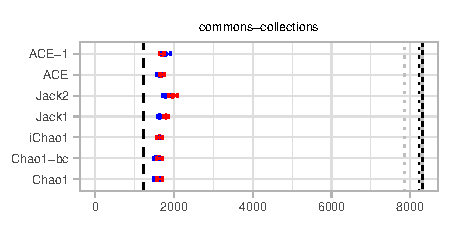
\includegraphics[width=0.9\linewidth]{charts_test/organic/commons-collections.pdf}
%        %\caption{1a}
%\end{subfigure}%
%\begin{subfigure}{.5\textwidth}
%    \centering
%      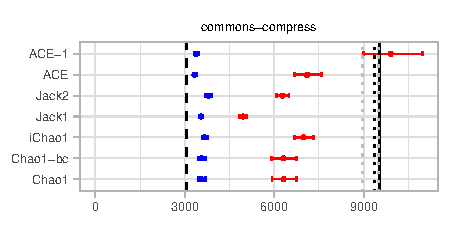
\includegraphics[width=0.9\linewidth]{charts_test/organic/commons-compress.pdf}
%        %\caption{1b}
%\end{subfigure}
%\begin{subfigure}{.5\textwidth}
%    \centering
%      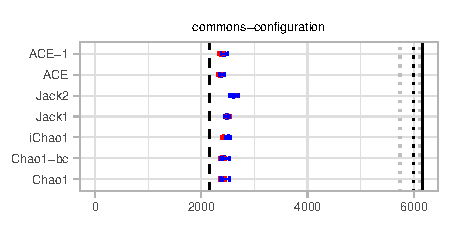
\includegraphics[width=0.9\linewidth]{charts_test/organic/commons-configuration.pdf}
%        %\caption{1b}
%\end{subfigure}%
%\begin{subfigure}{.5\textwidth}
%    \centering
%      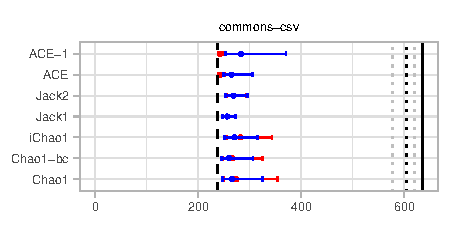
\includegraphics[width=0.9\linewidth]{charts_test/organic/commons-csv.pdf}
%        %\caption{1b}
%\end{subfigure}
%\begin{subfigure}{.5\textwidth}
%    \centering
%      \includegraphics[width=0.9\linewidth]{charts_test/organic/commons-dbcp.pdf}
%        %\caption{1b}
%\end{subfigure}%
%\begin{subfigure}{.5\textwidth}
%    \centering
%      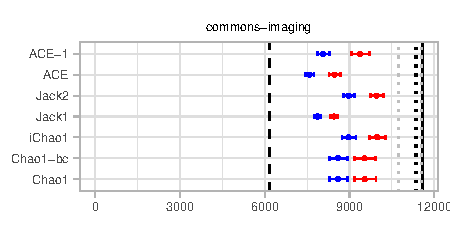
\includegraphics[width=0.9\linewidth]{charts_test/organic/commons-imaging.pdf}
%        %\caption{1b}
%\end{subfigure}
%\begin{subfigure}{.5\textwidth}
%    \centering
%      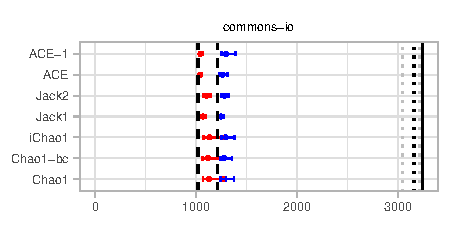
\includegraphics[width=0.9\linewidth]{charts_test/organic/commons-io.pdf}
%        %\caption{1b}
%\end{subfigure}%
%\begin{subfigure}{.5\textwidth}
%    \centering
%      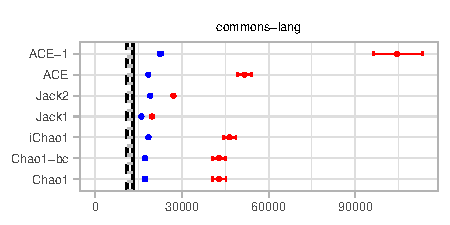
\includegraphics[width=0.9\linewidth]{charts_test/organic/commons-lang.pdf}
%        %\caption{1b}
%\end{subfigure}
%\begin{subfigure}{.5\textwidth}
%    \centering
%      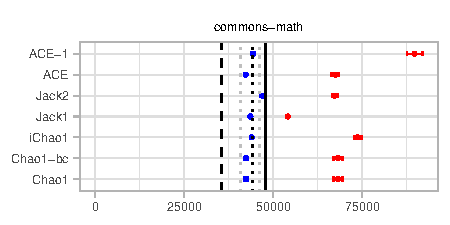
\includegraphics[width=0.9\linewidth]{charts_test/organic/commons-math.pdf}
%        %\caption{1b}
%\end{subfigure}%
%\begin{subfigure}{.5\textwidth}
%    \centering
%      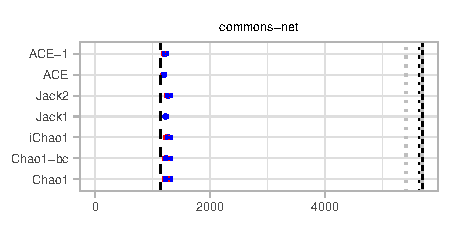
\includegraphics[width=0.9\linewidth]{charts_test/organic/commons-net.pdf}
%        %\caption{1b}
%\end{subfigure}
%  \caption{Estimators from test \original. The red is from \emph{class test set} data, and blue from \emph{method test set} data.}
%\label{fig:original}
%\end{figure*}

%
%
%\subsection{\EvosuiteRandom}
%\label{sec:random}
%\subsection{\EvosuiteStd}
%\label{sec:std}
%

%
%\subsection{Challenges Faced}
%During our empirical evaluation, we faced a number of challenges, and here is
%a list of some of the tougher challenges we faced.
%\begin{description}[leftmargin=0cm,labelindent=0cm]
%\item[Flacky tests.] Flaky tests were a major source of problems during our
%evaluation. In particular, tests that run and report no failure during manual
%runs sometimes fail during \PIT runs for extracting coverage.
%\item[Residual Errors in Classification.] We found that even after three fold confirmation,
%one of the mutants marked as equivalent was actually killed by an automatically
%generated test case.
%\item[\PIT bugs] The \PIT version we used sometimes resulted in corrupted XML
%files as output. Furthermore, \PIT would sometimes fail to detect bugs due to
%its incorrect coverage heuristics. We found that some such tests would detect
%mutants.
%\item[Sandboxes] When \PIT was used in programs that contained file IO, it
%often corrupted the file system, overwriting unintended files.
%\item[Bugs in R packages] Some of the statistical estimation packages had bugs
%in them, which we found thanks to implementing the estimation formulas
%ourselves and cross checking the results.
%\item[Limitations of \Evosuite] The \Evosuite test generator would not run on
%all programs we used.
%\end{description}
%

%\begin{figure*}
%\begin{subfigure}{.5\textwidth}
%    \centering
%      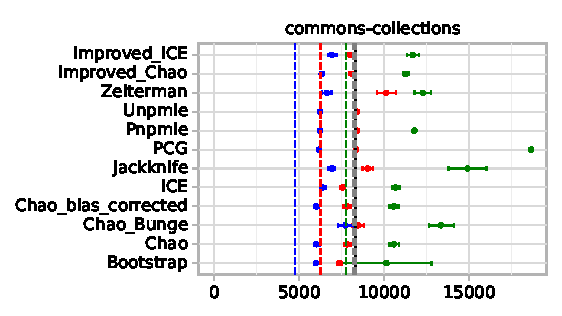
\includegraphics[width=0.9\linewidth]{charts/graph2/graph2/commons-collections.pdf}
%        %\caption{1a}
%\end{subfigure}%
%\begin{subfigure}{.5\textwidth}
%    \centering
%      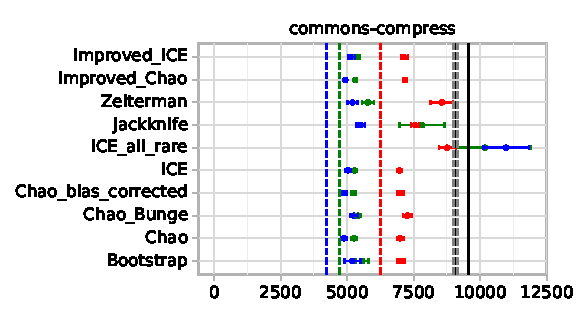
\includegraphics[width=0.9\linewidth]{charts/graph2/graph2/commons-compress.pdf}
%        %\caption{1b}
%\end{subfigure}
%\begin{subfigure}{.5\textwidth}
%    \centering
%      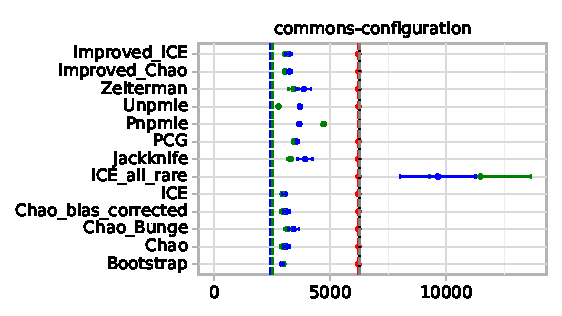
\includegraphics[width=0.9\linewidth]{charts/graph2/graph2/commons-configuration.pdf}
%        %\caption{1b}
%\end{subfigure}%
%\begin{subfigure}{.5\textwidth}
%    \centering
%      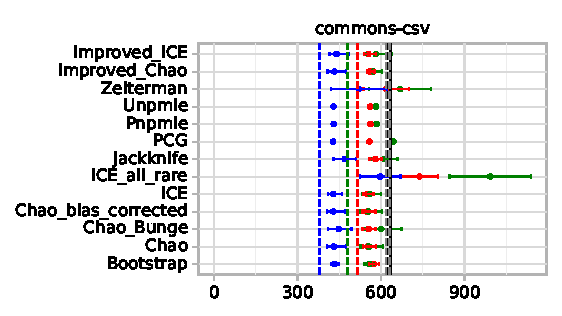
\includegraphics[width=0.9\linewidth]{charts/graph2/graph2/commons-csv.pdf}
%        %\caption{1b}
%\end{subfigure}
%\begin{subfigure}{.5\textwidth}
%    \centering
%      \includegraphics[width=0.9\linewidth]{charts/graph2/graph2/commons-dbcp.pdf}
%        %\caption{1b}
%\end{subfigure}%
%\begin{subfigure}{.5\textwidth}
%    \centering
%      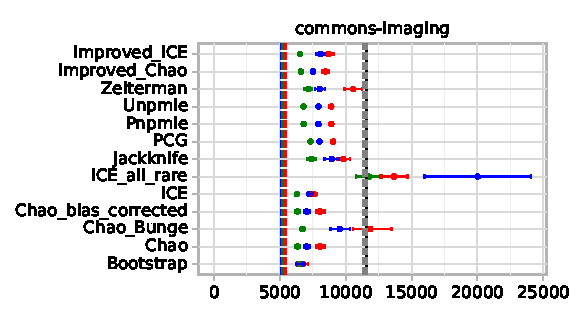
\includegraphics[width=0.9\linewidth]{charts/graph2/graph2/commons-imaging.pdf}
%        %\caption{1b}
%\end{subfigure}
%\begin{subfigure}{.5\textwidth}
%    \centering
%      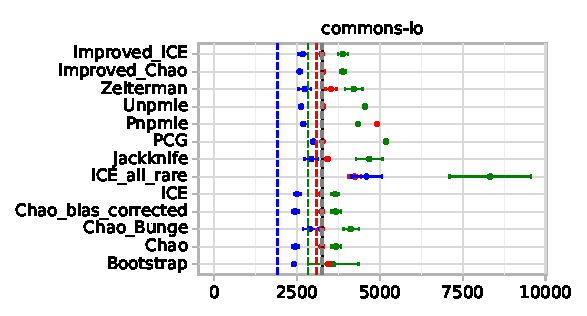
\includegraphics[width=0.9\linewidth]{charts/graph2/graph2/commons-io.pdf}
%        %\caption{1b}
%\end{subfigure}%
%\begin{subfigure}{.5\textwidth}
%    \centering
%      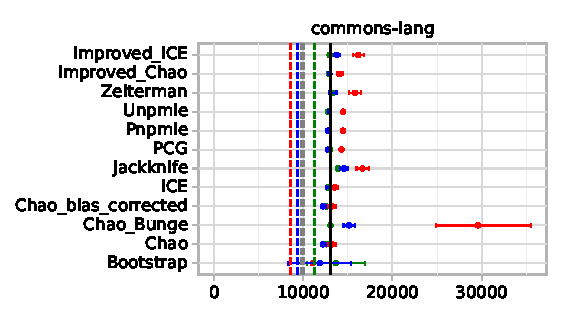
\includegraphics[width=0.9\linewidth]{charts/graph2/graph2/commons-lang.pdf}
%        %\caption{1b}
%\end{subfigure}
%\begin{subfigure}{.5\textwidth}
%    \centering
%      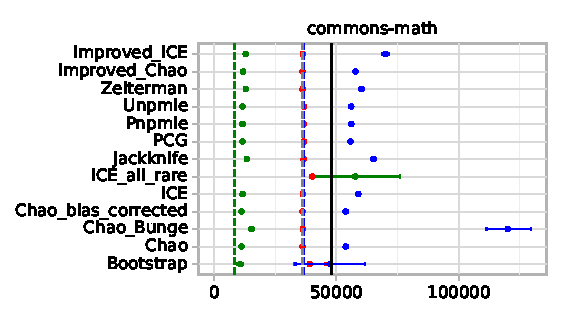
\includegraphics[width=0.9\linewidth]{charts/graph2/graph2/commons-math.pdf}
%        %\caption{1b}
%\end{subfigure}%
%\begin{subfigure}{.5\textwidth}
%    \centering
%      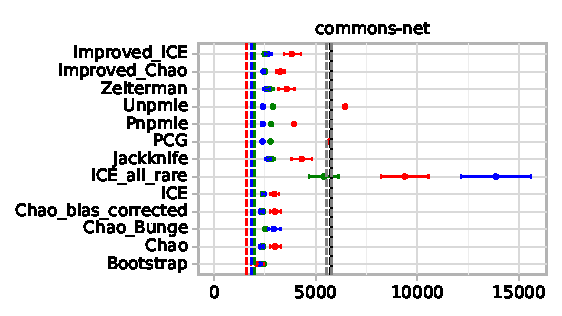
\includegraphics[width=0.9\linewidth]{charts/graph2/graph2/commons-net.pdf}
%        %\caption{1b}
%\end{subfigure}
%  \caption{method test data, with test suites indicated by color.
%  \original is \textcolor{red}{red}, \EvosuiteRandom is \textcolor{blue}{blue}
%  and \EvosuiteDynamosa is \textcolor{green}{green}.
%  Dashed lines represent killed mutants by respective test cases,
%  and error bars represent estimates from
%  mutant kills by each estimator. The solid black line is the total mutants
%  generated, dashed black line the manual estimate, and gray dashed lines the
%  error bars.}
%\label{fig:testmethods}
%\end{figure*}
%
%
%\begin{figure*}
%\begin{subfigure}{\textwidth}
%    \centering
%      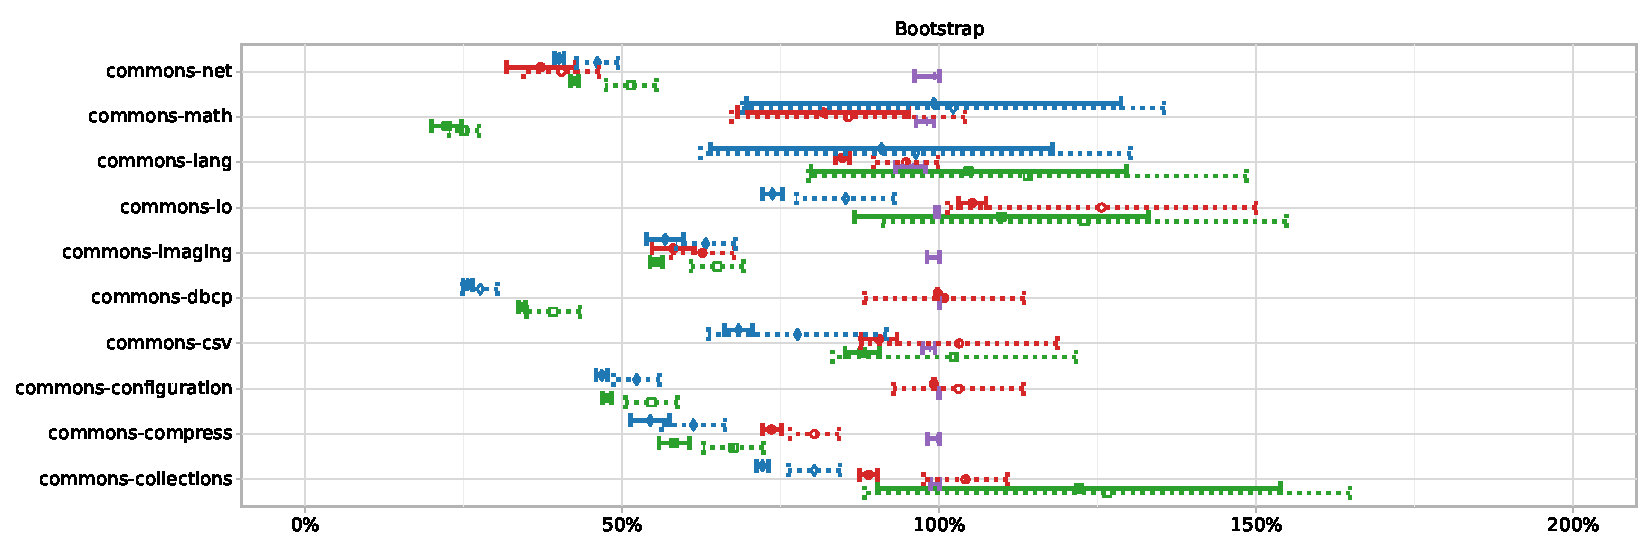
\includegraphics[width=0.9\linewidth]{estimators/Bootstrap.pdf}
%        %\caption{1a}
%\end{subfigure}
%\begin{subfigure}{\textwidth}
%    \centering
%      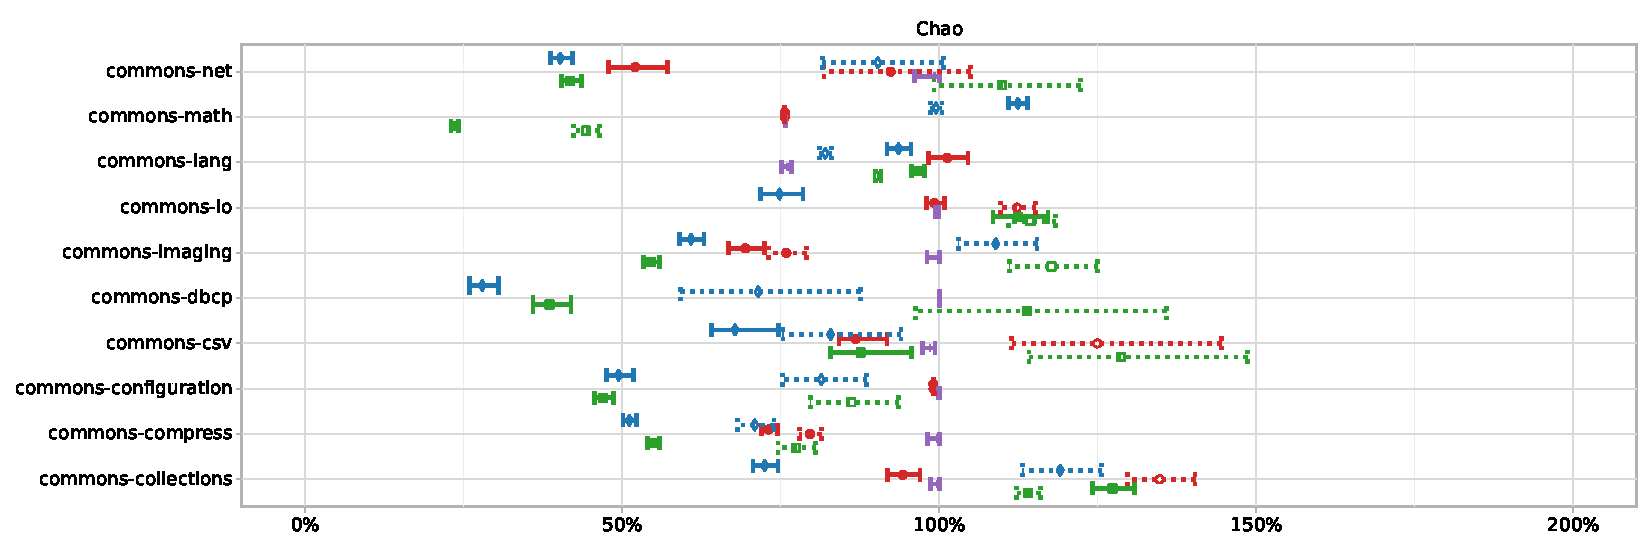
\includegraphics[width=0.9\linewidth]{estimators/Chao.pdf}
%        %\caption{1b}
%\end{subfigure}
%\begin{subfigure}{\textwidth}
%    \centering
%      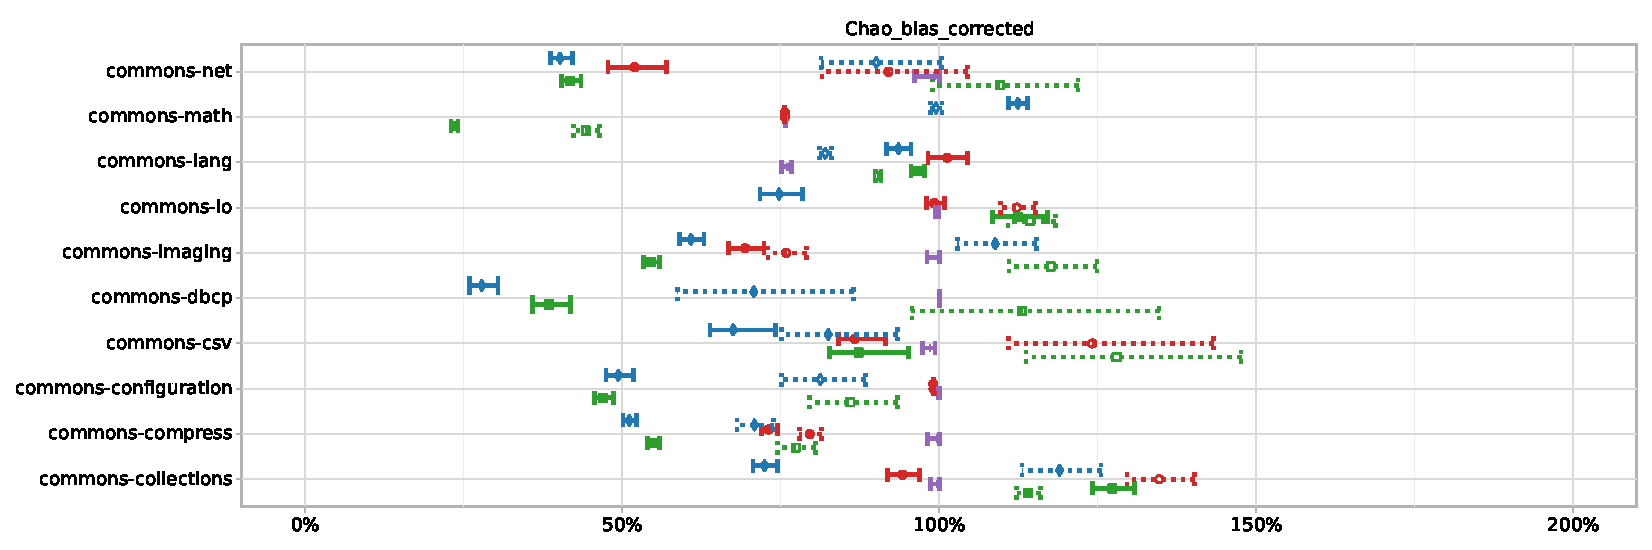
\includegraphics[width=0.9\linewidth]{estimators/Chao_bias_corrected.pdf}
%        %\caption{1b}
%\end{subfigure}
%\begin{subfigure}{\textwidth}
%    \centering
%      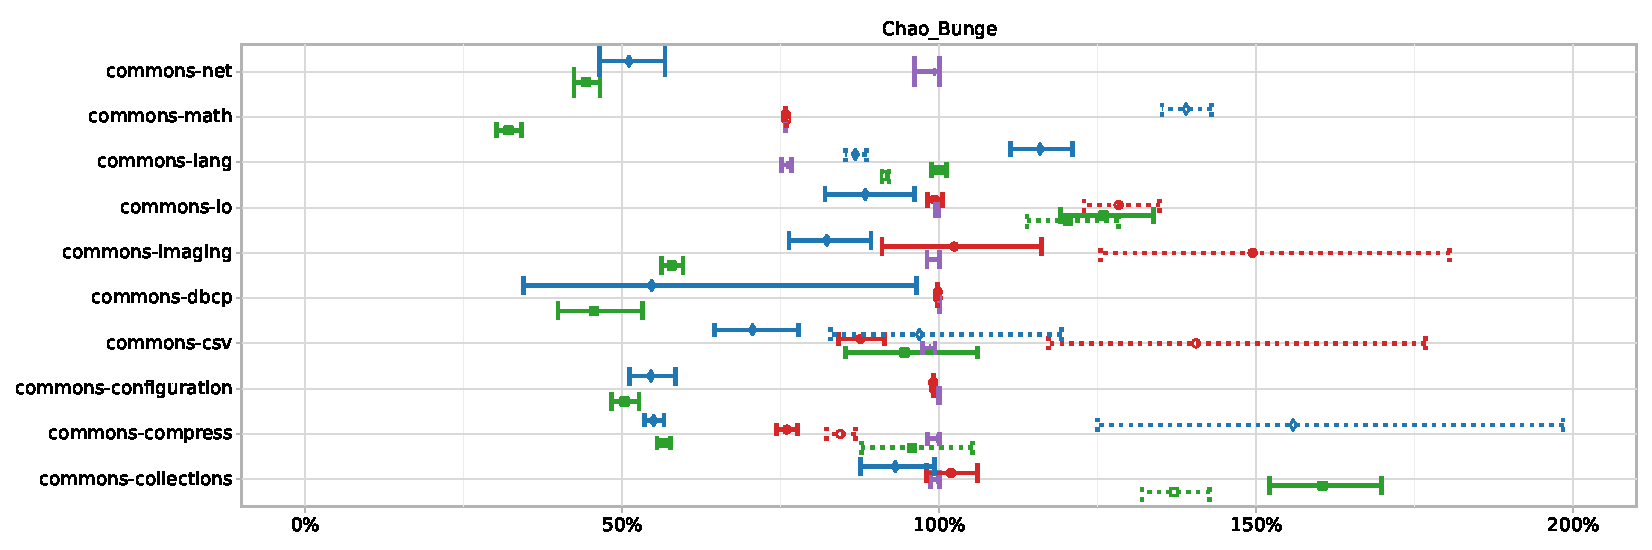
\includegraphics[width=0.9\linewidth]{estimators/Chao_Bunge.pdf}
%        %\caption{1b}
%\end{subfigure}
%  \caption{test data, with test suites indicated by color.
%  The manual classification is in \textcolor{purple}{purple}.
%  \original is \textcolor{red}{red}, \EvosuiteRandom is \textcolor{blue}{blue}
%  and \EvosuiteDynamosa is \textcolor{green}{green}.
%  Dashed lines represent estimates and errorbars from class based samples
%  while solid lines represent estimates and errorbars from method based
%  samples.
% } 
%\label{fig:estimates}
%\end{figure*}
%
%
%\begin{figure*}
%\begin{subfigure}{\textwidth}
%    \centering
%      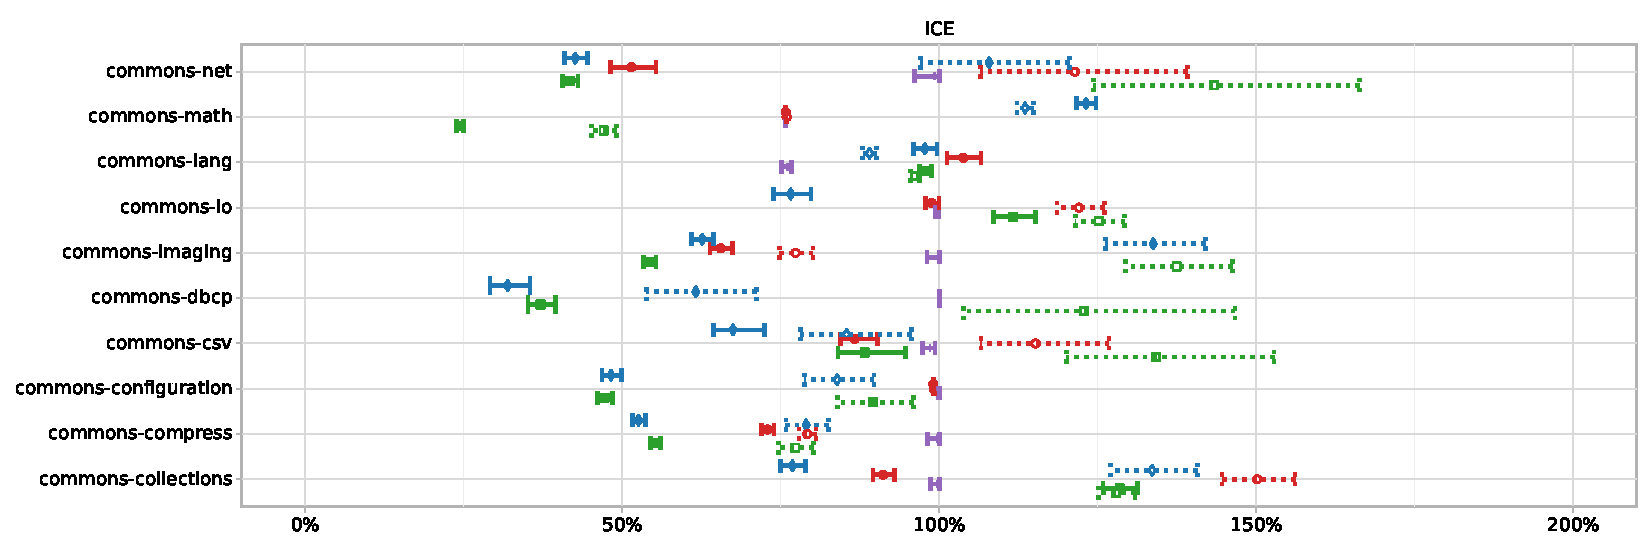
\includegraphics[width=0.9\linewidth]{estimators/ICE.pdf}
%        %\caption{1b}
%\end{subfigure}
%\begin{subfigure}{\textwidth}
%    \centering
%      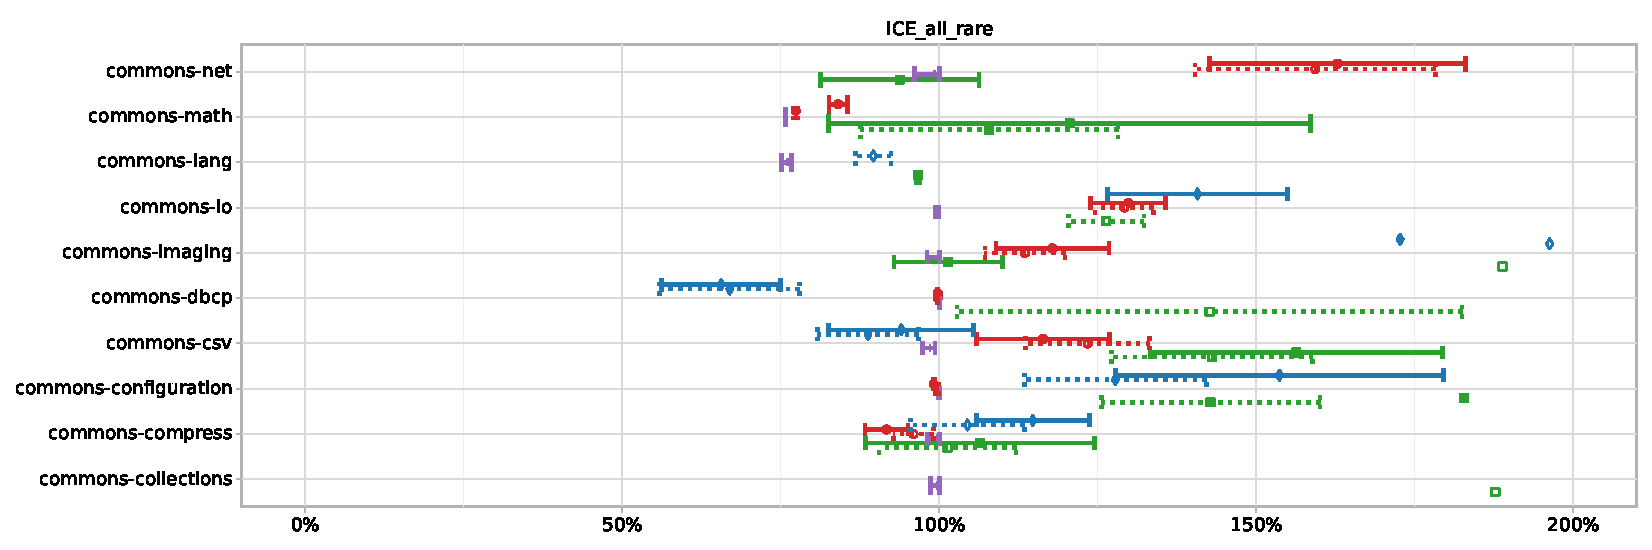
\includegraphics[width=0.9\linewidth]{estimators/ICE_all_rare.pdf}
%        %\caption{1b}
%\end{subfigure}
%\begin{subfigure}{\textwidth}
%    \centering
%      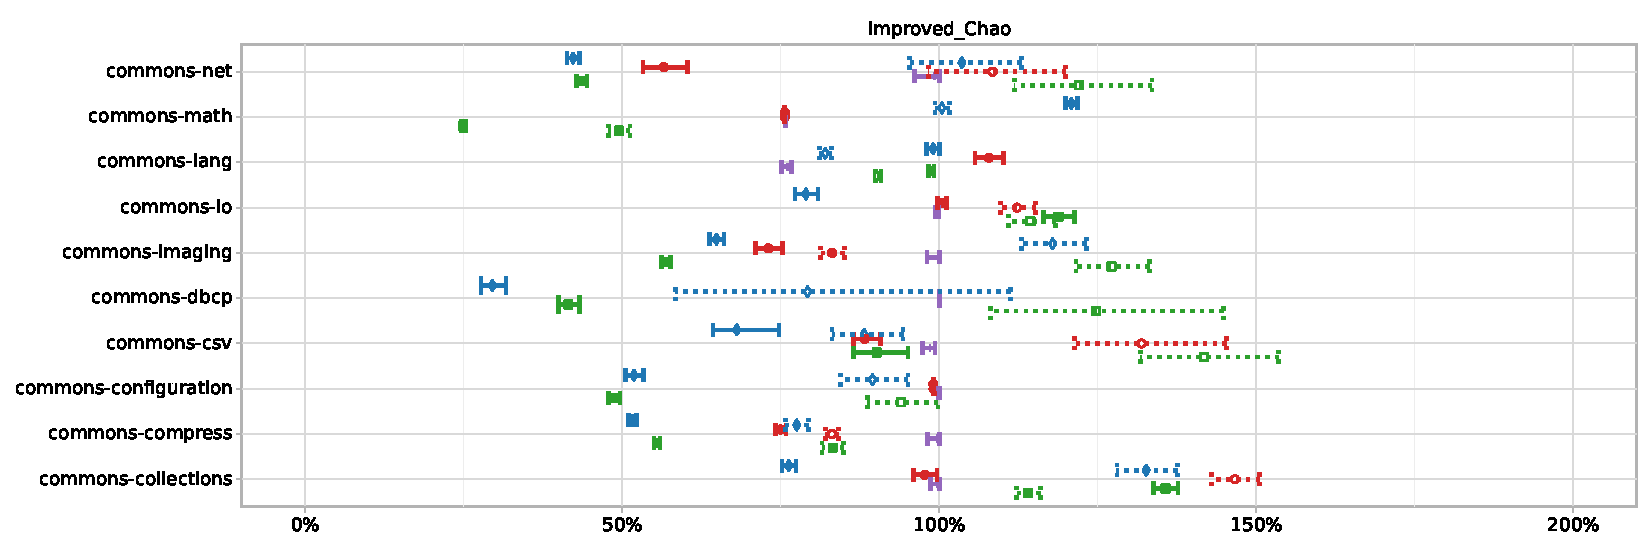
\includegraphics[width=0.9\linewidth]{estimators/improved_Chao.pdf}
%        %\caption{1b}
%\end{subfigure}
%\begin{subfigure}{\textwidth}
%    \centering
%      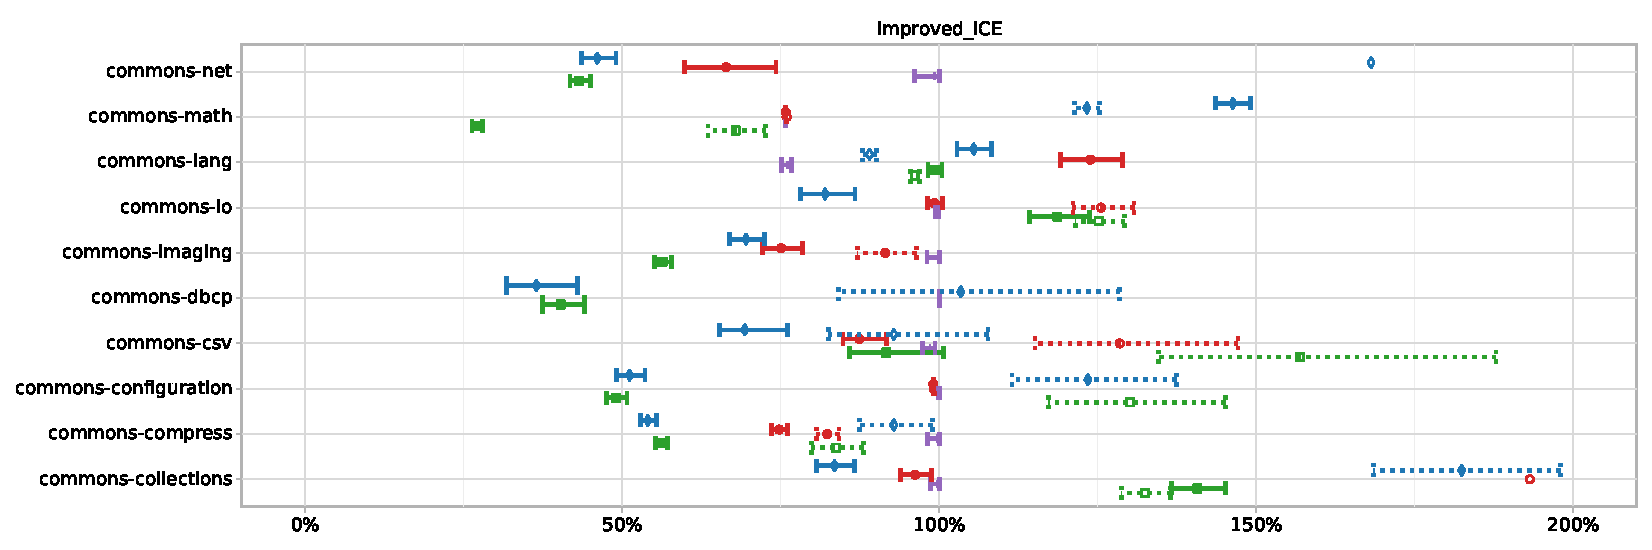
\includegraphics[width=0.9\linewidth]{estimators/improved_ICE.pdf}
%        %\caption{1b}
%\end{subfigure}
%% \begin{subfigure}{\textwidth}
%%     \centering
%%       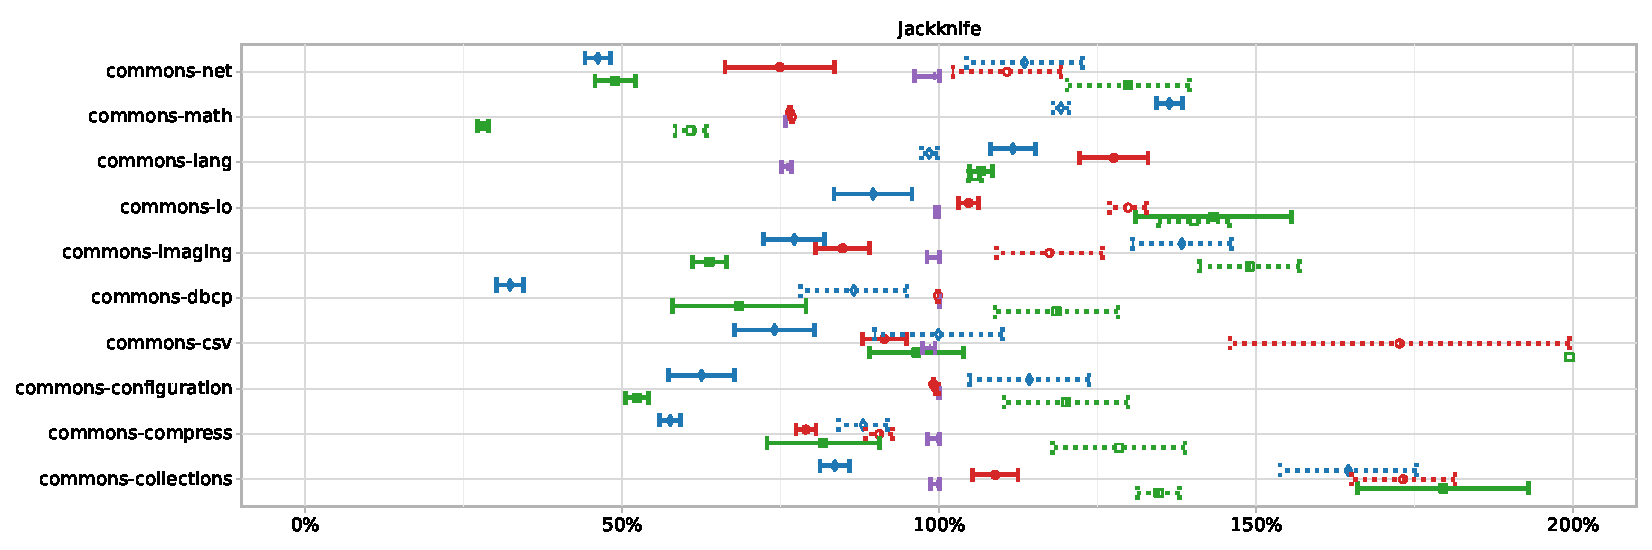
\includegraphics[width=0.9\linewidth]{estimators/Jackknife.pdf}
%%         %\caption{1b}
%% \end{subfigure}
%% \begin{subfigure}{\textwidth}
%%     \centering
%%       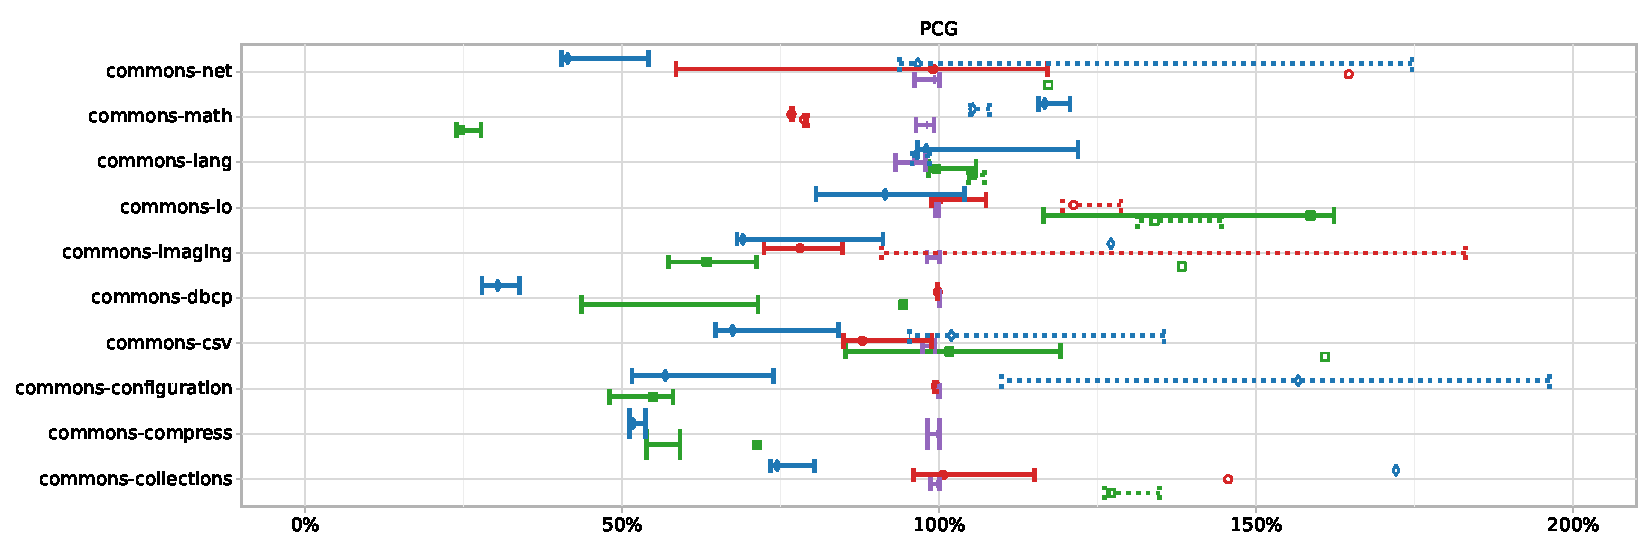
\includegraphics[width=0.9\linewidth]{estimators/PCG.pdf}
%%         %\caption{1b}
%% \end{subfigure}
%  \caption{test data, with test suites indicated by color.
%  The manual classification is in \textcolor{purple}{purple}.
%  \original is \textcolor{red}{red}, \EvosuiteRandom is \textcolor{blue}{blue}
%  and \EvosuiteDynamosa is \textcolor{green}{green}.
%  Dashed lines represent estimates and errorbars from class based samples
%  while solid lines represent estimates and errorbars from method based
%  samples.
% } 
%\label{fig:estimates2}
%\end{figure*}
%
%\begin{figure*}
%\begin{subfigure}{\textwidth}
%    \centering
%      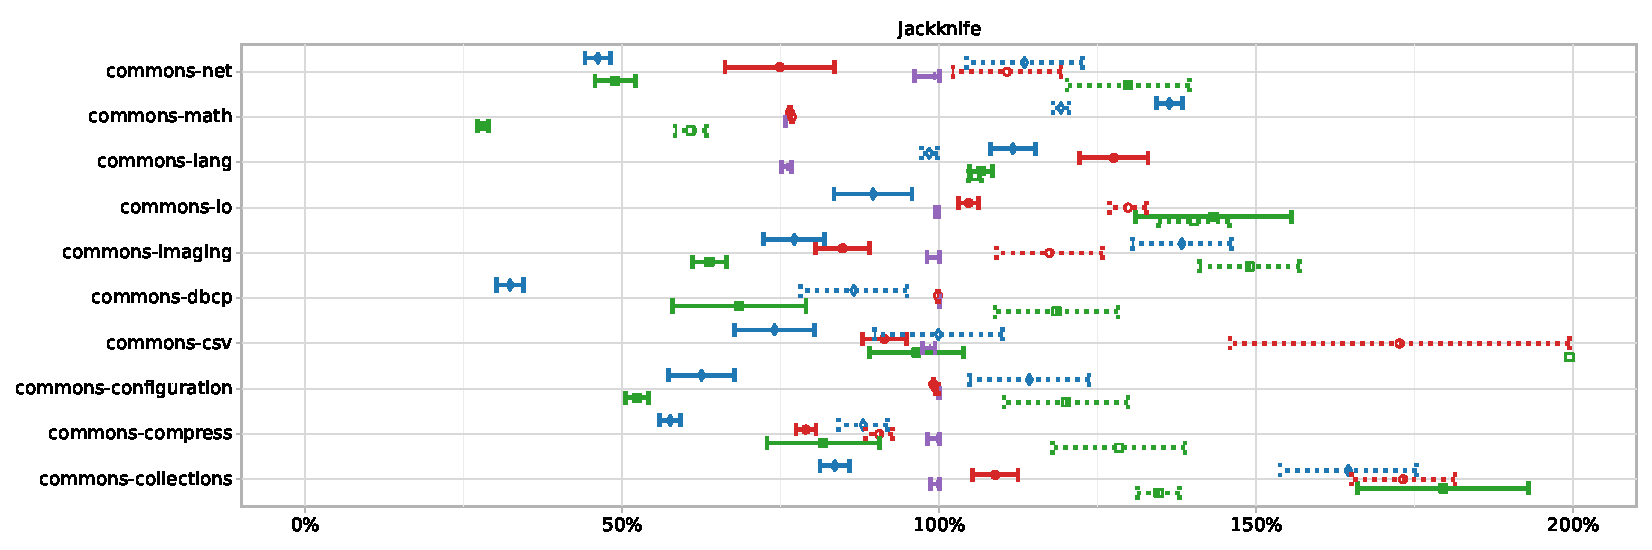
\includegraphics[width=0.9\linewidth]{estimators/Jackknife.pdf}
%        %\caption{1b}
%\end{subfigure}
%\begin{subfigure}{\textwidth}
%    \centering
%      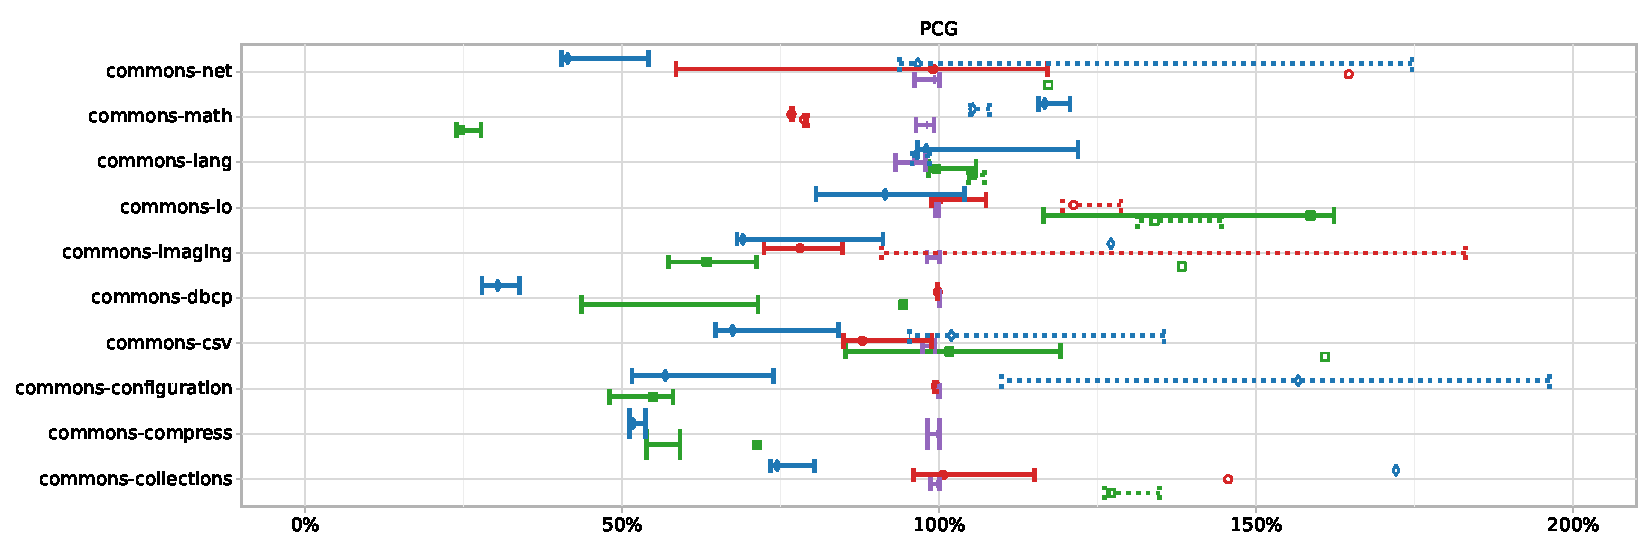
\includegraphics[width=0.9\linewidth]{estimators/PCG.pdf}
%        %\caption{1b}
%\end{subfigure}
%\begin{subfigure}{\textwidth}
%    \centering
%      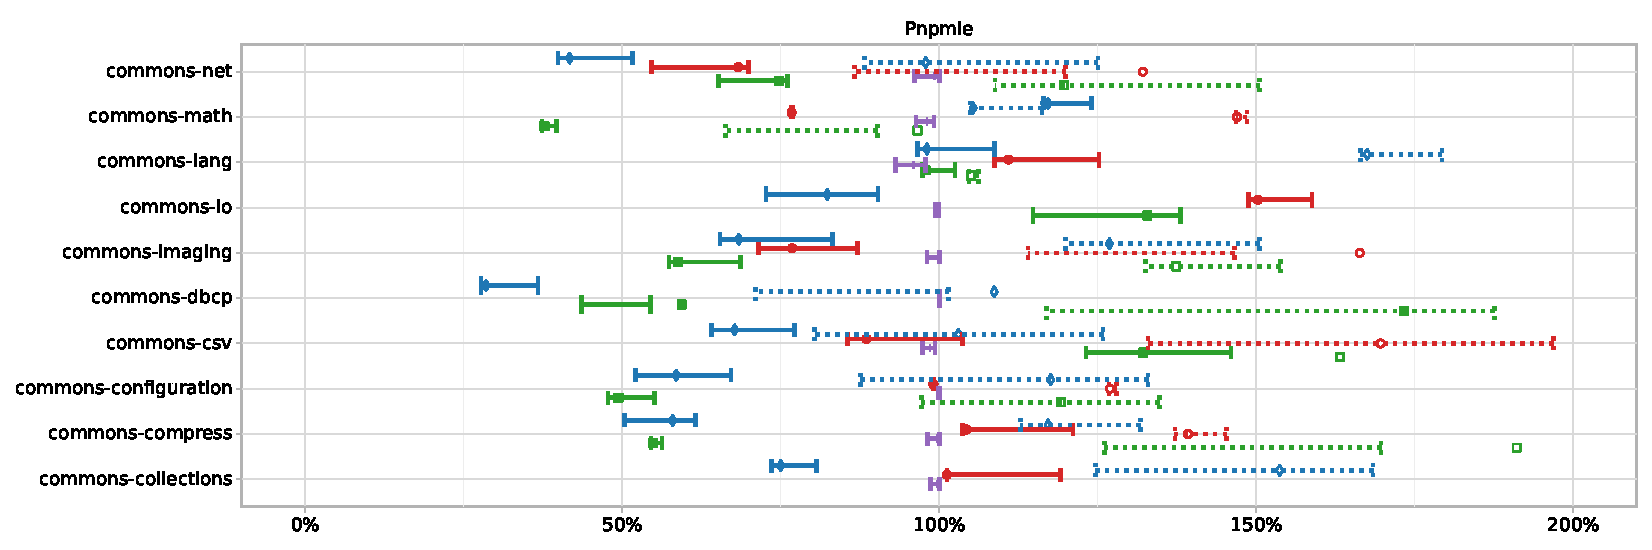
\includegraphics[width=0.9\linewidth]{estimators/Pnpmle.pdf}
%        %\caption{1b}
%\end{subfigure}
%\begin{subfigure}{\textwidth}
%    \centering
%      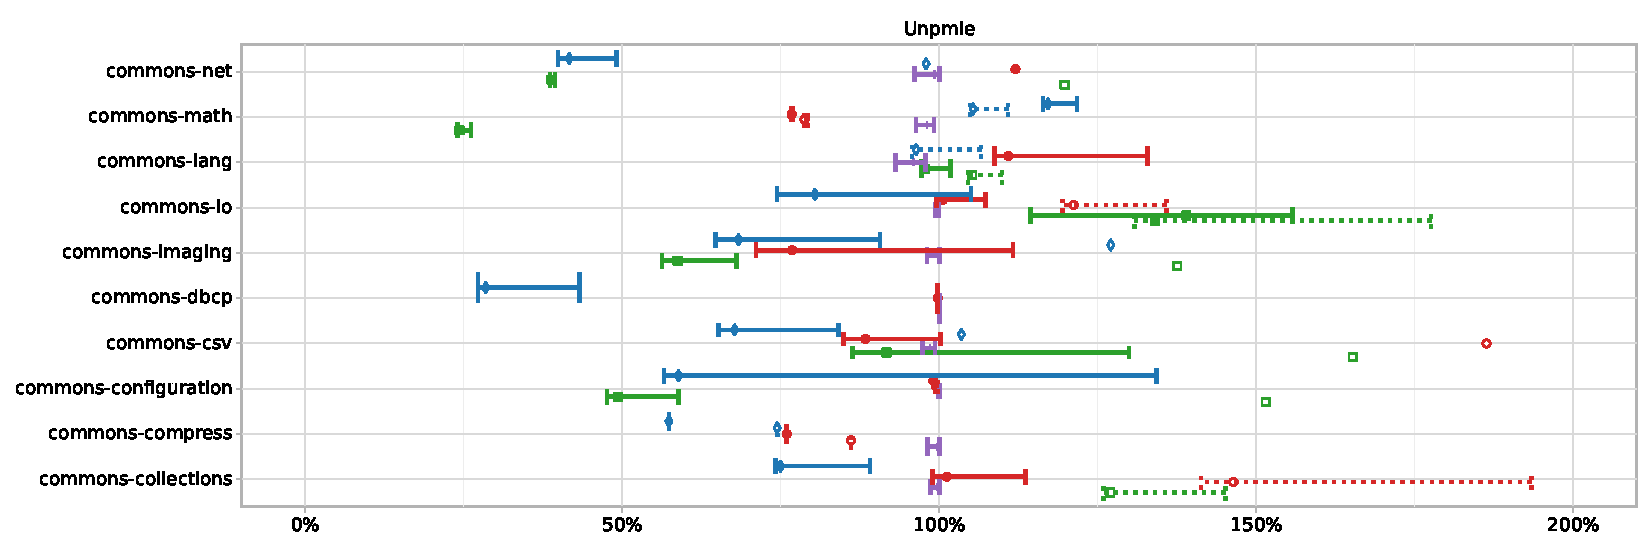
\includegraphics[width=0.9\linewidth]{estimators/Unpmle.pdf}
%        %\caption{1b}
%\end{subfigure}
%%\begin{subfigure}{\textwidth}
%%    \centering
%%      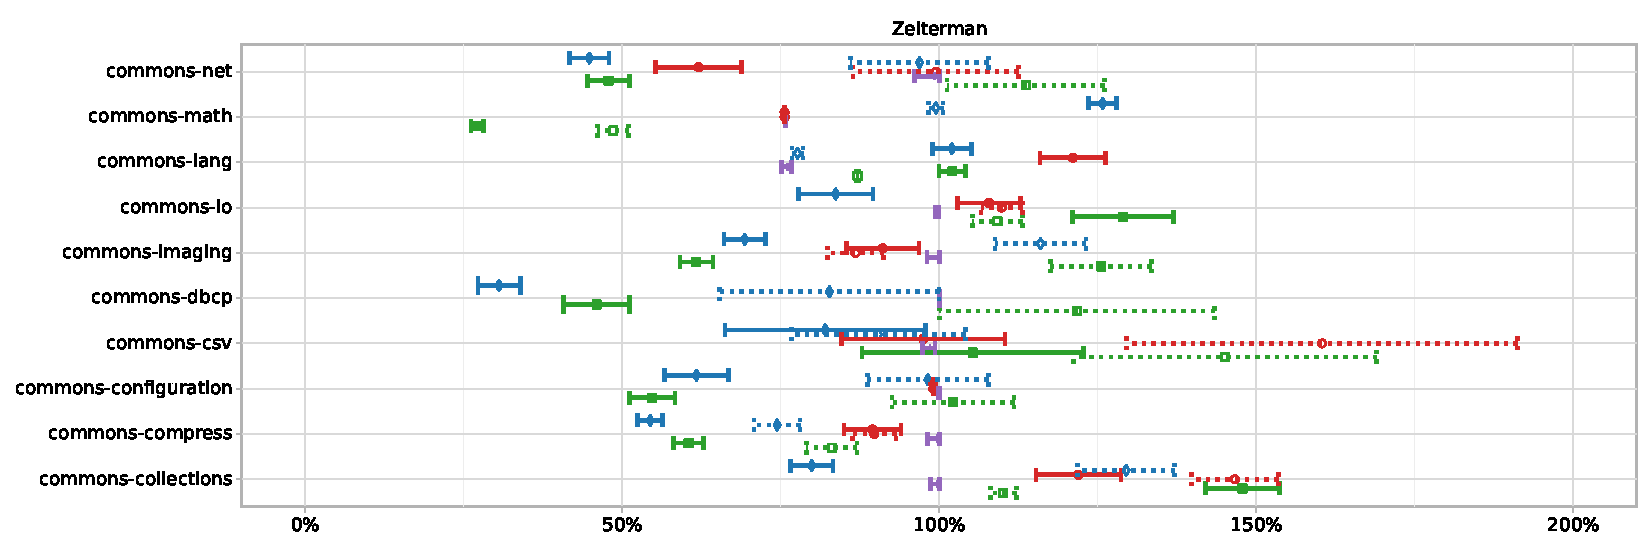
\includegraphics[width=0.9\linewidth]{estimators/Zelterman.pdf}
%%        %\caption{1b}
%%\end{subfigure}
%  \caption{test data, with test suites indicated by color.
%  The manual classification is in \textcolor{purple}{purple}.
%  \original is \textcolor{red}{red}, \EvosuiteRandom is \textcolor{blue}{blue}
%  and \EvosuiteDynamosa is \textcolor{green}{green}.
%  Dashed lines represent estimates and errorbars from class based samples
%  while solid lines represent estimates and errorbars from method based
%  samples.
% } 
%\label{fig:estimates3}
%\end{figure*}
%\begin{figure*}
%\begin{subfigure}{\textwidth}
%    \centering
%      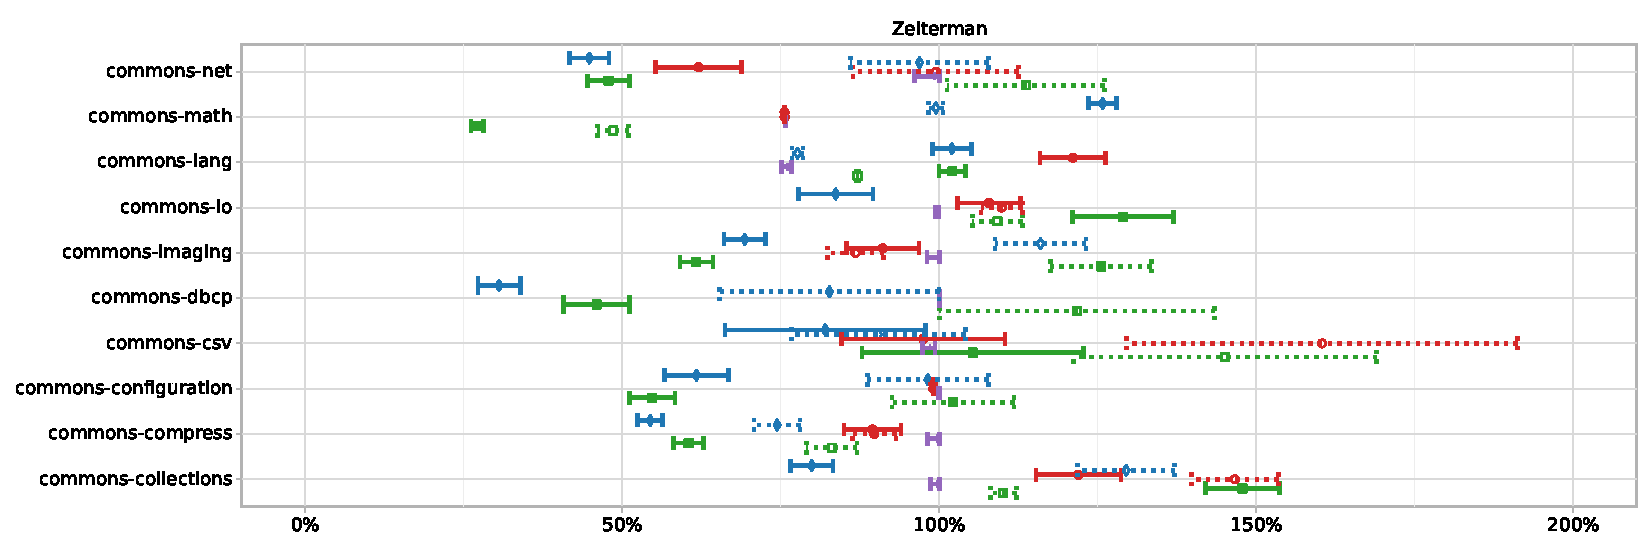
\includegraphics[width=0.9\linewidth]{estimators/Zelterman.pdf}
%        %\caption{1b}
%\end{subfigure}
%  \caption{test data, with test suites indicated by color.
%  The manual classification is in \textcolor{purple}{purple}.
%  \original is \textcolor{red}{red}, \EvosuiteRandom is \textcolor{blue}{blue}
%  and \EvosuiteDynamosa is \textcolor{green}{green}.
%  Dashed lines represent estimates and errorbars from class based samples
%  while solid lines represent estimates and errorbars from method based
%  samples.
% } 
%\label{fig:estimates4}
%\end{figure*}


%\maketitle
\end{document}
\endinput
